\documentclass{article}
\usepackage[utf8]{inputenc}
\usepackage{fancyhdr}
\usepackage{graphicx}
\usepackage{geometry}
\usepackage{tikz}
\usepackage{rotating}


% ---- Commands ------- %
\newcommand{\documentNumber}[1]{
    \LARGE  \textbf{ PUSS2142{#1} } \\
    \medskip
}
\newcommand{\documentVersion}[1]{
    v. {#1}

    \medskip
}
\newcommand{\documentTitle}[1]{
    \centerline{\rule{13cm}{0.4pt}}
    \bigskip \bigskip
    \LARGE \textbf{TimeMate} \\
    \bigskip
    \LARGE {#1} \\
    \bigskip \bigskip
    \centerline{\rule{13cm}{0.4pt}}
}
\newcommand{\documentGroup}[1]{
    \bigskip \bigskip
    \LARGE Group {#1} \\
    \bigskip
}
\newcommand{\documentResponsible}[1]{
    \LARGE Responsible: {#1} \\
    \medskip
}
\newcommand{\documentAuthors}[1]{
    \LARGE Authors: {#1} \\
    \medskip    
}
\newcommand{\documentDate}[1]{
    \date {#1} 
}

\graphicspath{{./images/}} % Defines a path to file images
\renewcommand{\arraystretch}{1.7}  % Vertical padding for tables


% --- Header & Footer ---- %
\pagestyle{fancy}
\lhead{\leftmark}
\rhead{}
\rfoot{\thepage}
\cfoot{}
\lfoot{}


% ------------------------------------------------ #

% ----- FILL THIS ----- %
\title {
    % Must be 2 digits
    \documentNumber {06}    
    
    % BASELINE.VERSION
    \documentVersion {0.1}
    
    % Full name - SHORTNAME
    \documentTitle {Software Verification and Validation Report}
    \documentGroup {2}
    
    % Options: - Project Management Group
    %          - System Architecture Group
    %          - Developer Group
    %          - Test Group
    \documentResponsible {Test Group}
    \documentAuthors {Test Group}
    
    % Format: YYYY-MM-DD
    \documentDate {2021-03-03}
}

\begin{document}

\maketitle
\thispagestyle{empty}

\newpage

\tableofcontents

\newpage

%---------Document begins here-----------

% FILL IN CORRECT VERSION HISTORY!
% Not sure? Refer to SDP how it works or ask someone!
\section{Document History}
\begin{tabular}{ l | l | l | l }
    Version & Date & Responsible & Description \\
    \hline
  	0.1 & 2021-01-03 & TG & Document created. \\
   % 0.2 & 2021-02-02 & PG & Ready for informal review. \\
   % 0.3 & 2021-02-04 & PG & Fixed gramatical changes and typos. \\
\end{tabular}

\section{Overview}

\section{Test Process}

\section{Appendices}
\begin{itemize}
\item \textbf{A.} Function Test Result
\item \textbf{B.} System Test Result
\item \textbf{C.} Regression Test Result 
\item \textbf{D.} Test Result in Google Sheet
\item \textbf{E.} Review Protocols
\end{itemize}

\newpage
\begin{flushleft}
{\large\textbf{A. Function Test Result}}
\end{flushleft}

\vspace*{\fill}
                \hfill
                \begin{center}
                This page unintentionally left blank.
                \end{center}
                \vspace{\fill}
                \thispagestyle{empty}

\begin{figure}
     \centering
     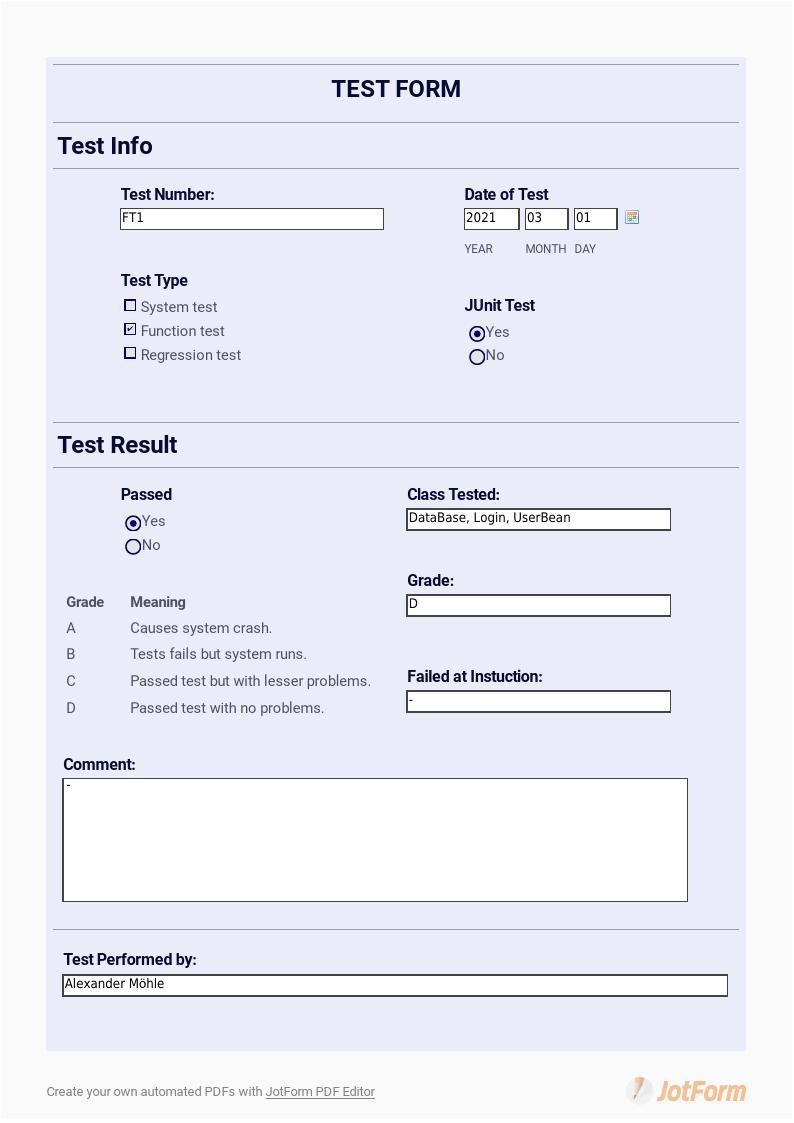
\includegraphics[width=13cm]{images/2021_03_01_Alexander_FT1_001}
     \renewcommand\figurename{Figure}
     \caption{Test form for FT1}
     \label{fig:my_label}
 \end{figure}
 
 \begin{figure}
     \centering
     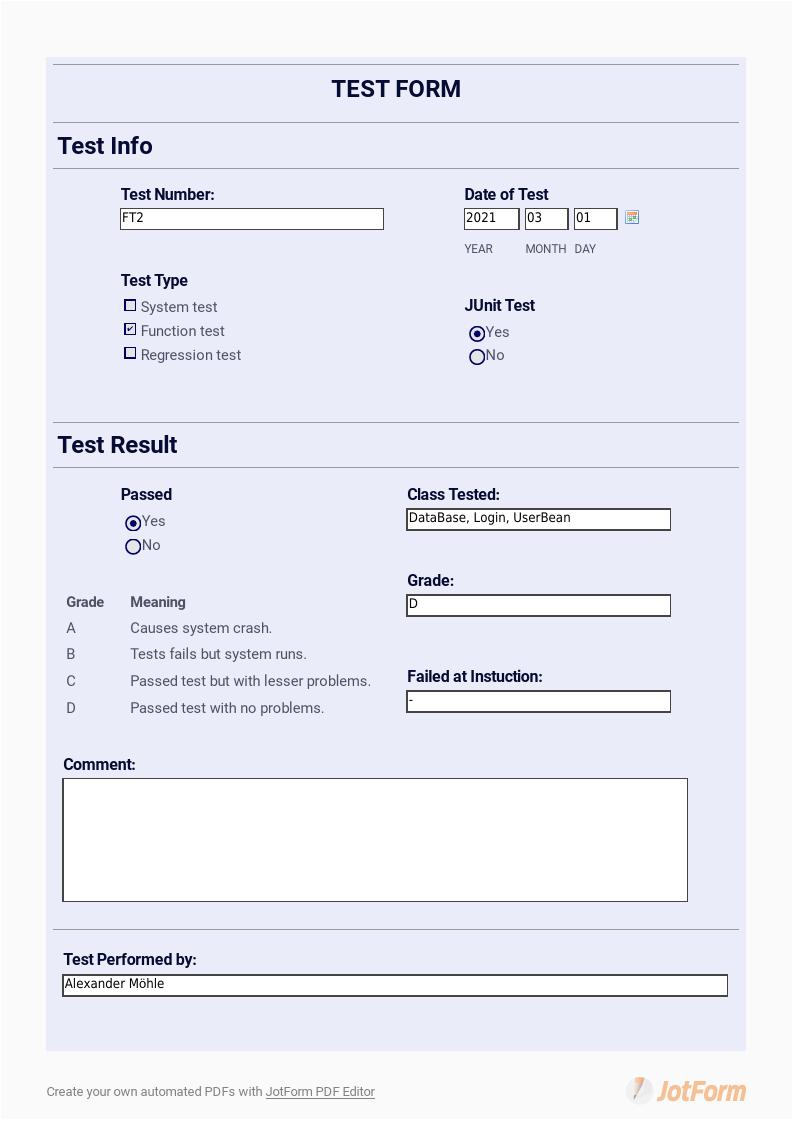
\includegraphics[width=13cm]{images/2021-03-01_Alexander_FT2_001}
     \renewcommand\figurename{Figure}
     \caption{Test form for FT2}
     \label{fig:my_label}
 \end{figure}
 
  \begin{figure}
     \centering
     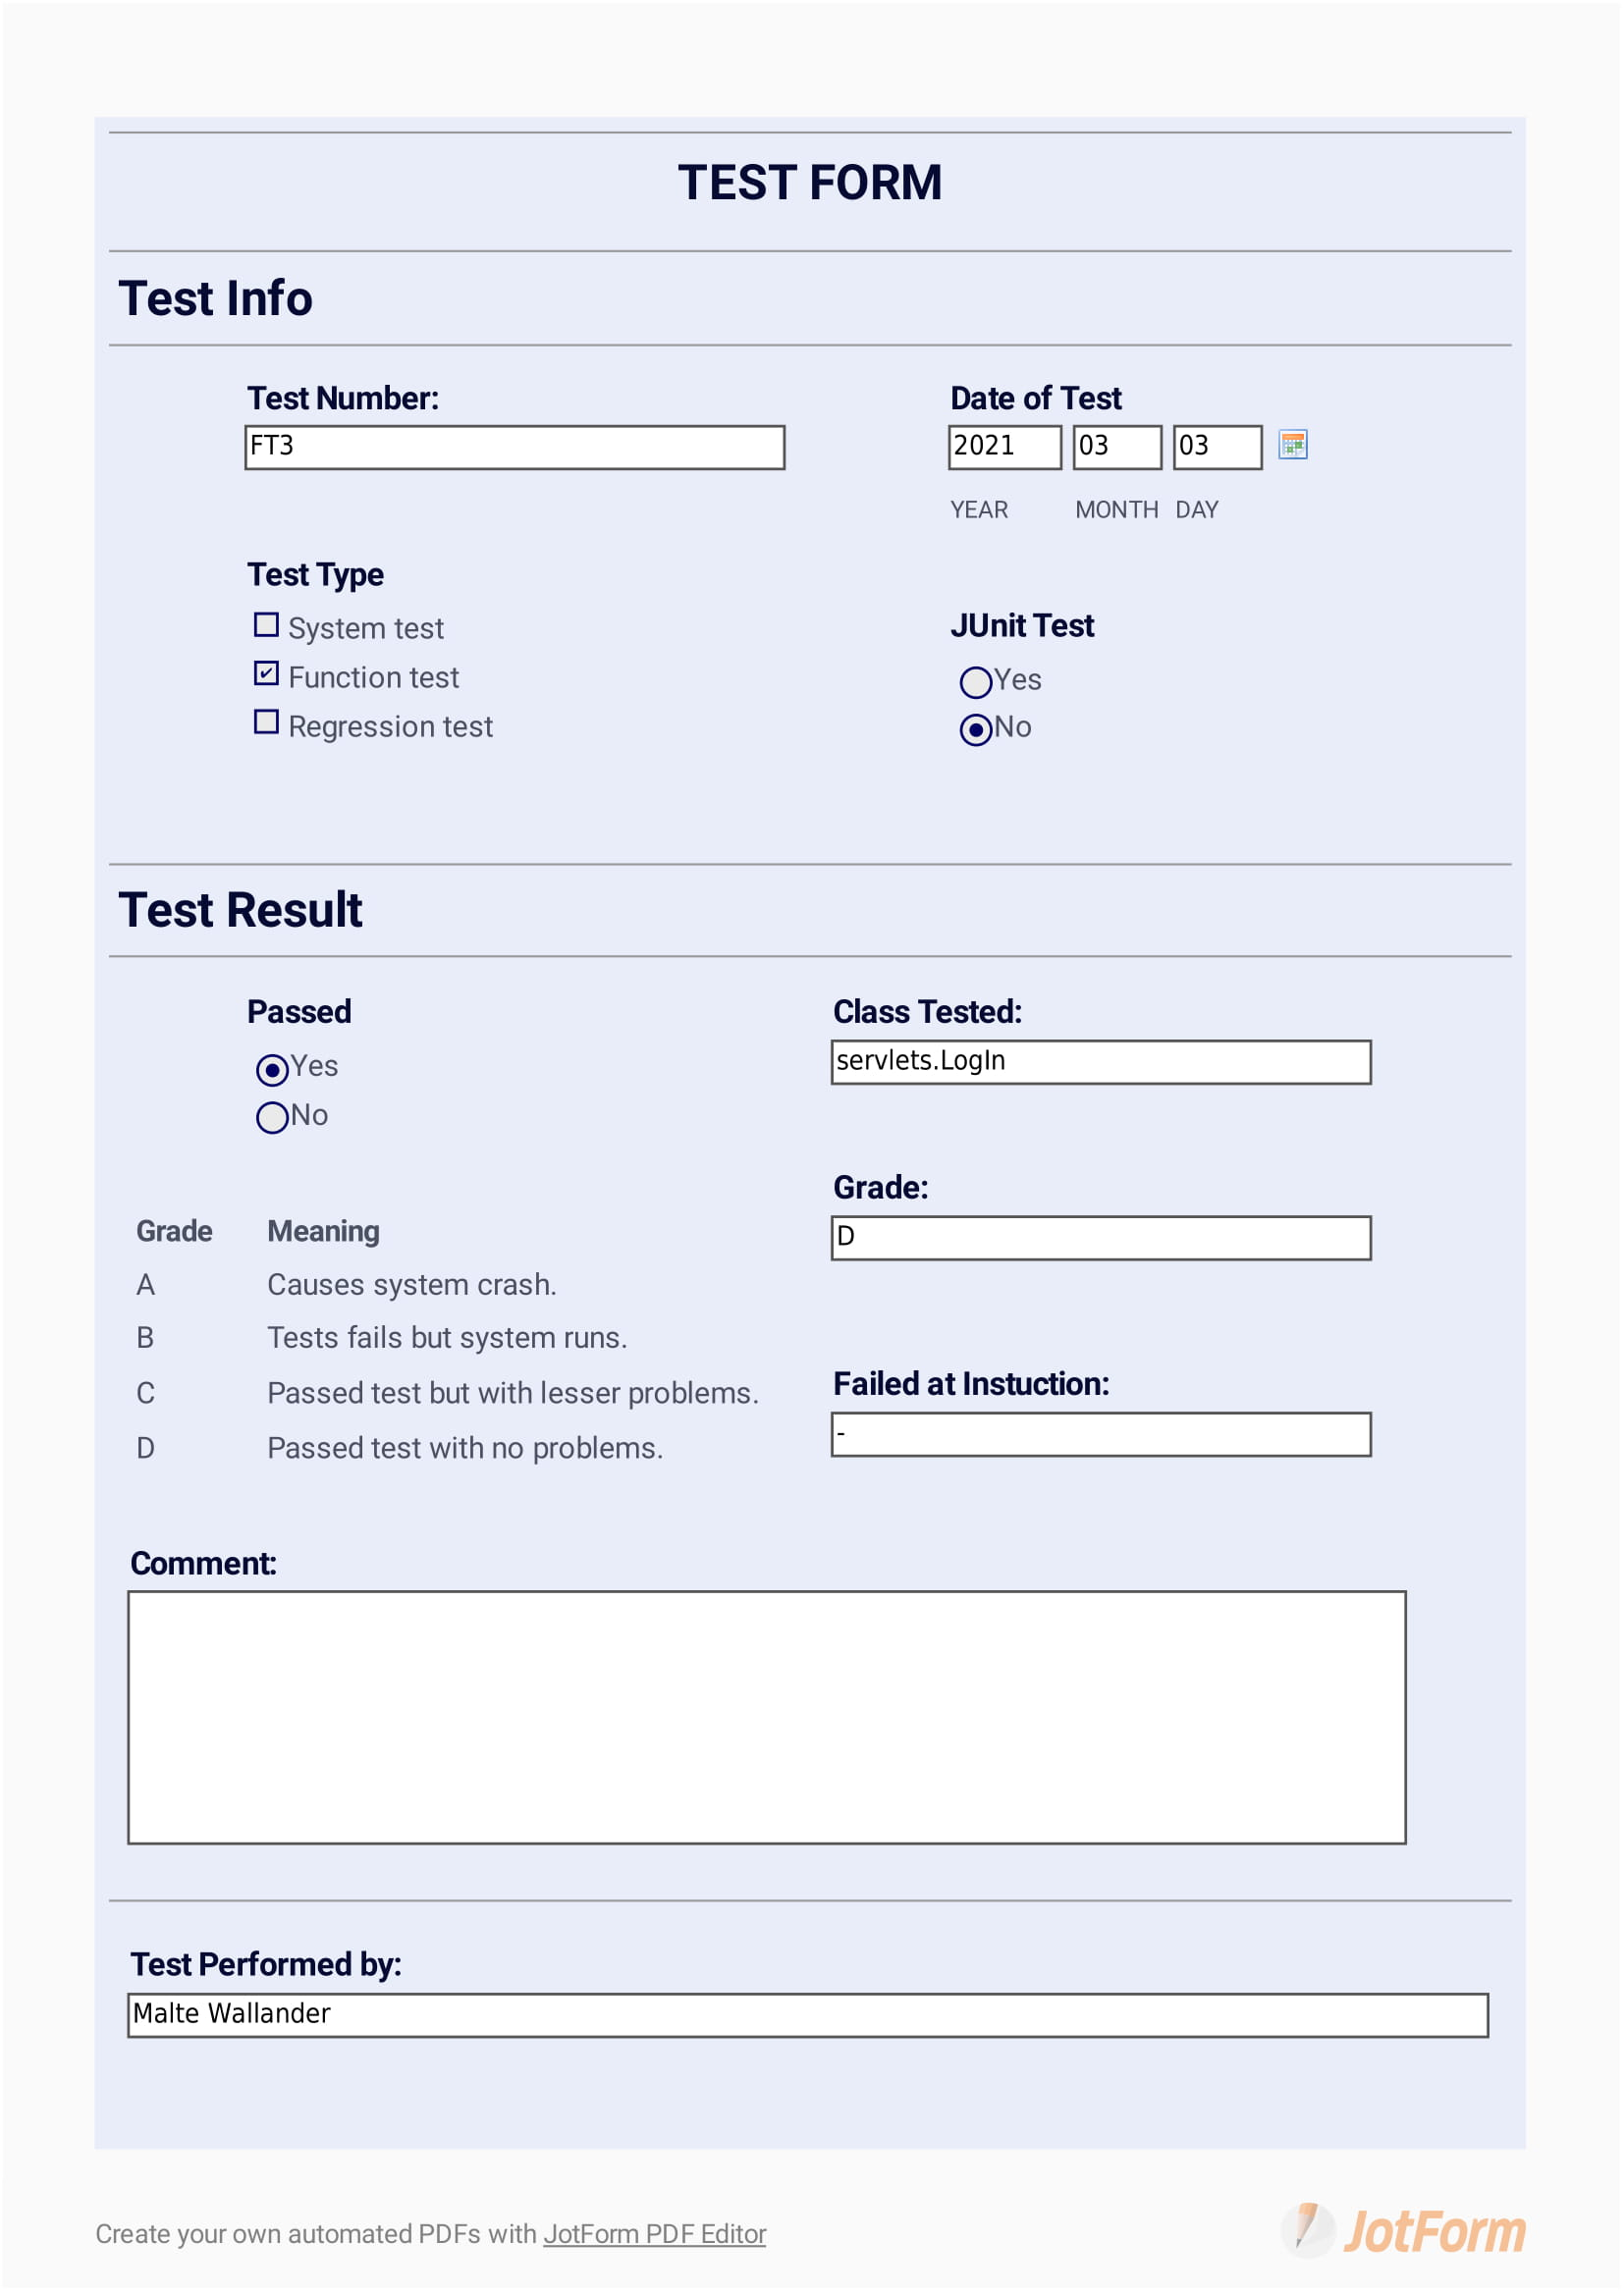
\includegraphics[width=13cm]{images/2021-03-03_Malte_FT3-1}
     \renewcommand\figurename{Figure}
     \caption{Test form for FT3}
     \label{fig:my_label}
 \end{figure}
 
 \begin{figure}
     \centering
     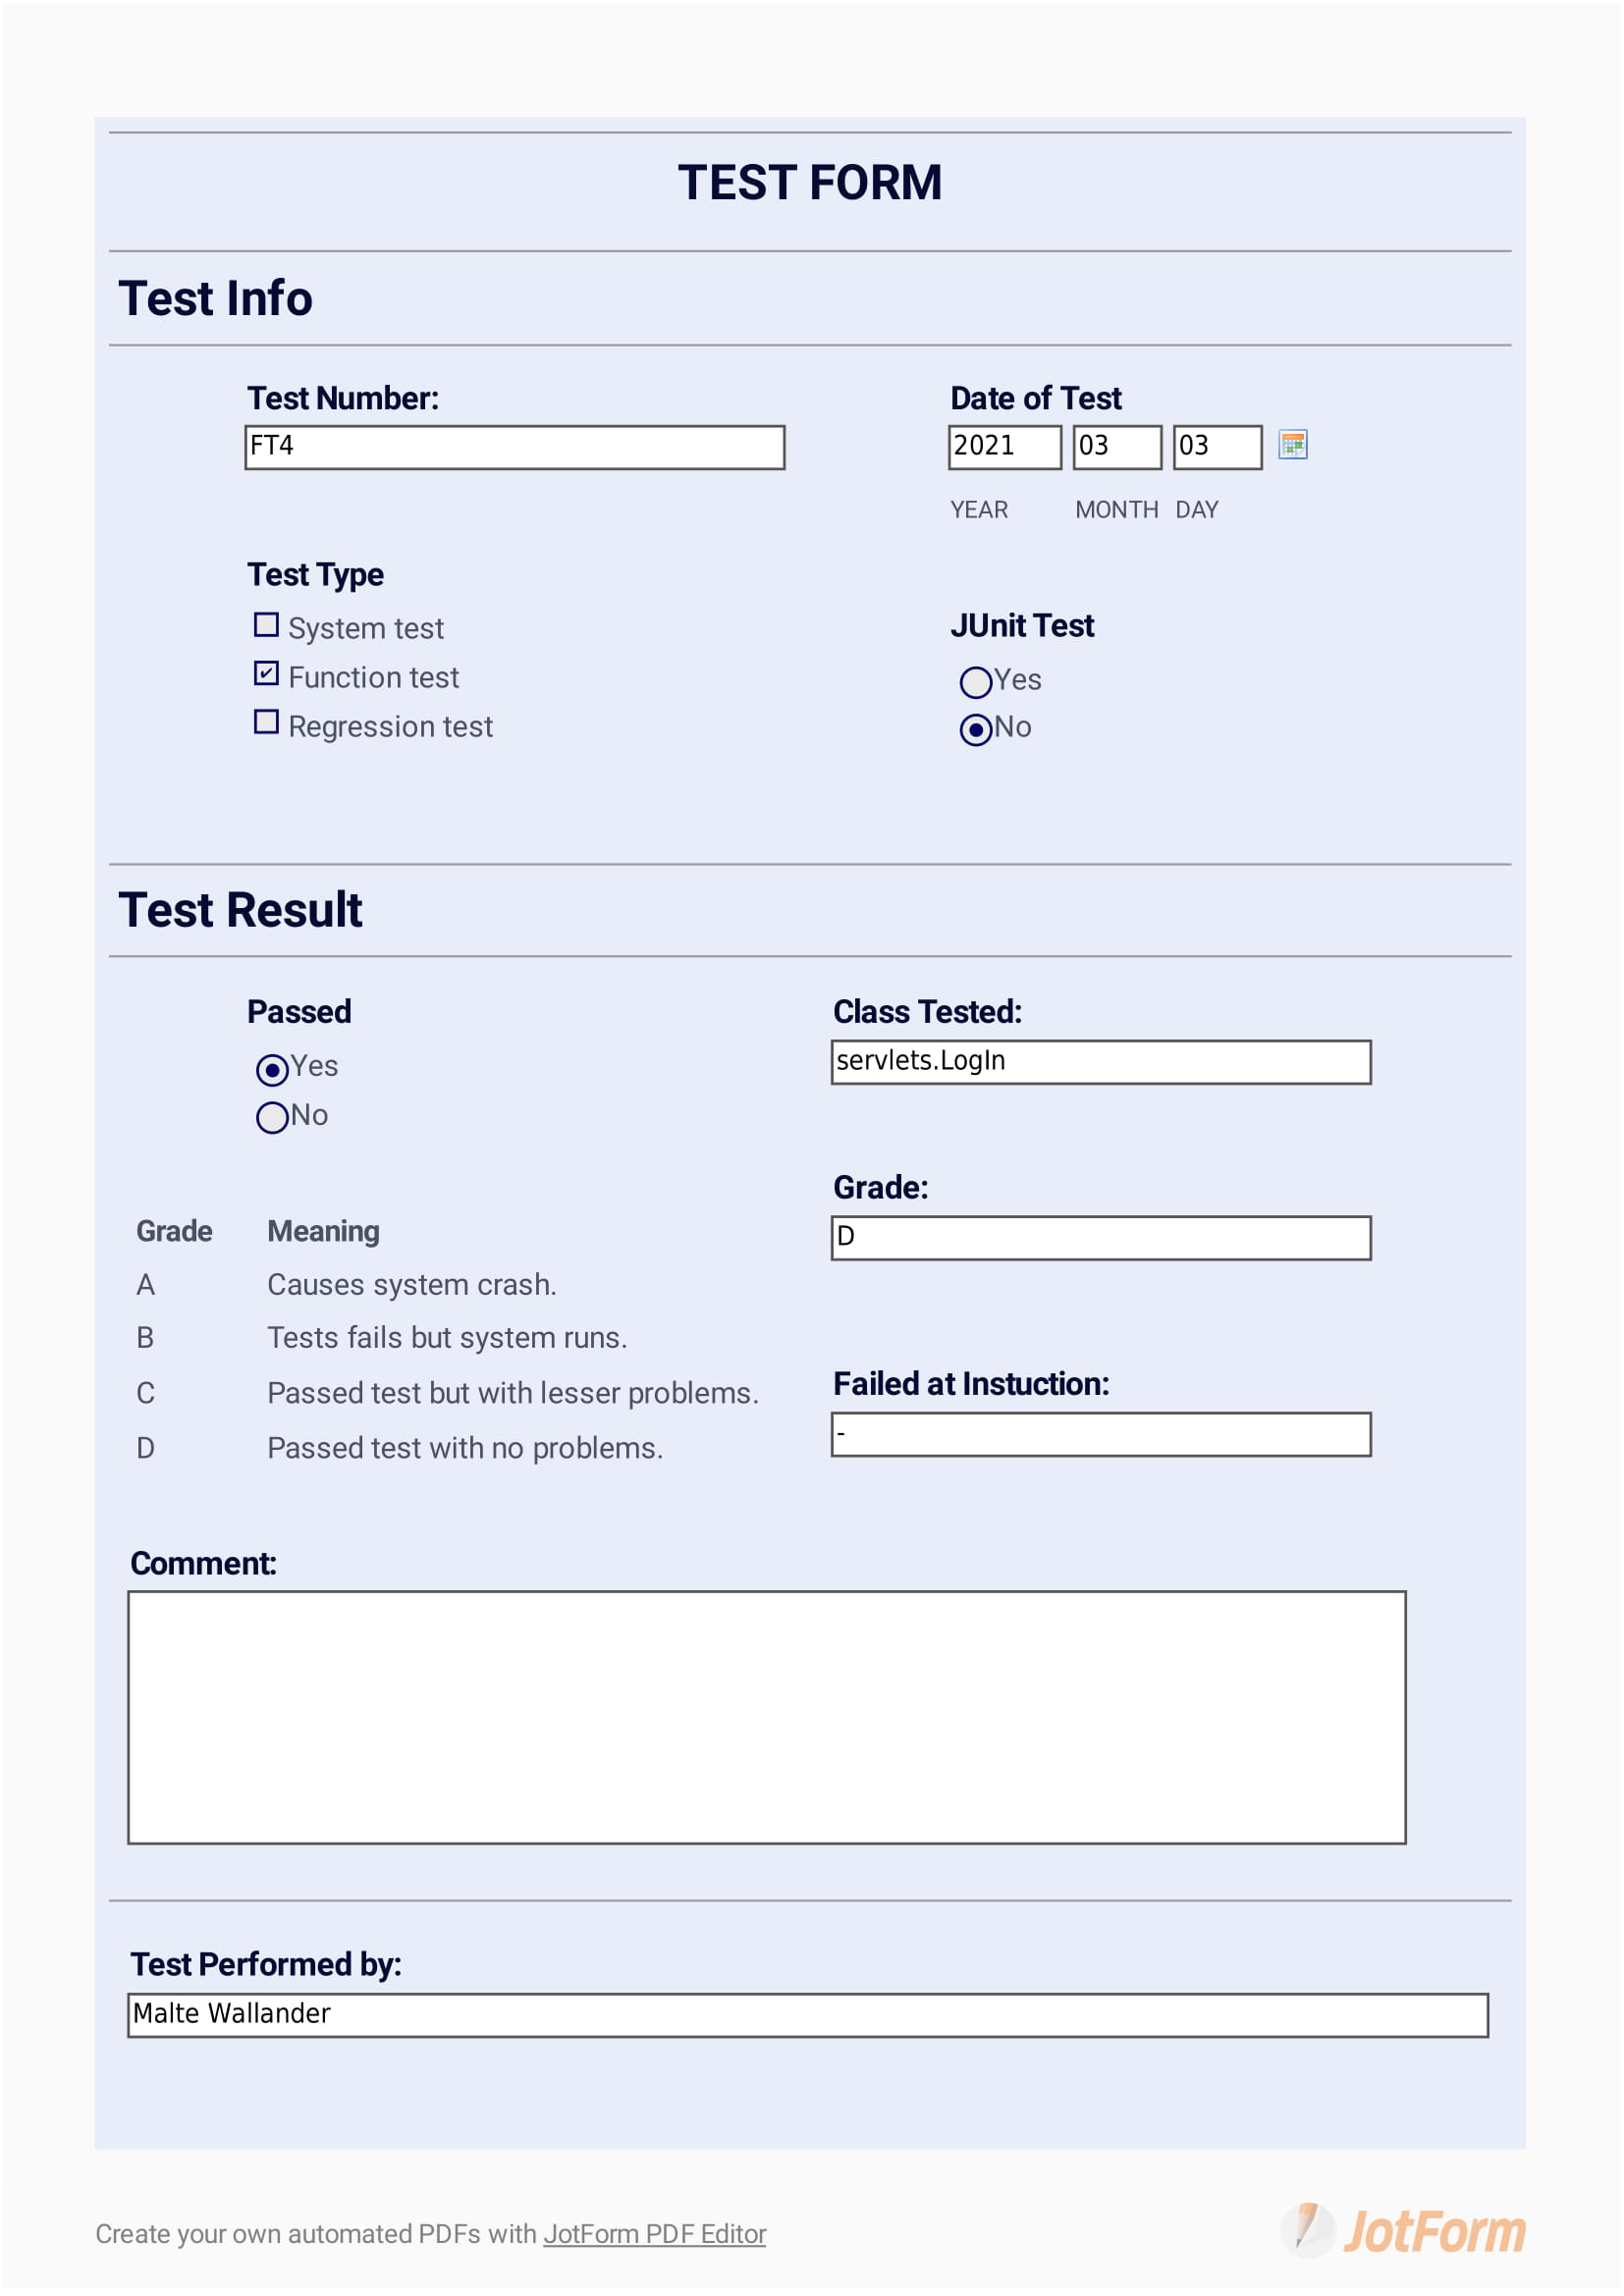
\includegraphics[width=13cm]{images/2021-03-03_Malte_FT4-1}
     \renewcommand\figurename{Figure}
     \caption{Test form for FT4}
     \label{fig:my_label}
 \end{figure}

\begin{figure}
     \centering
     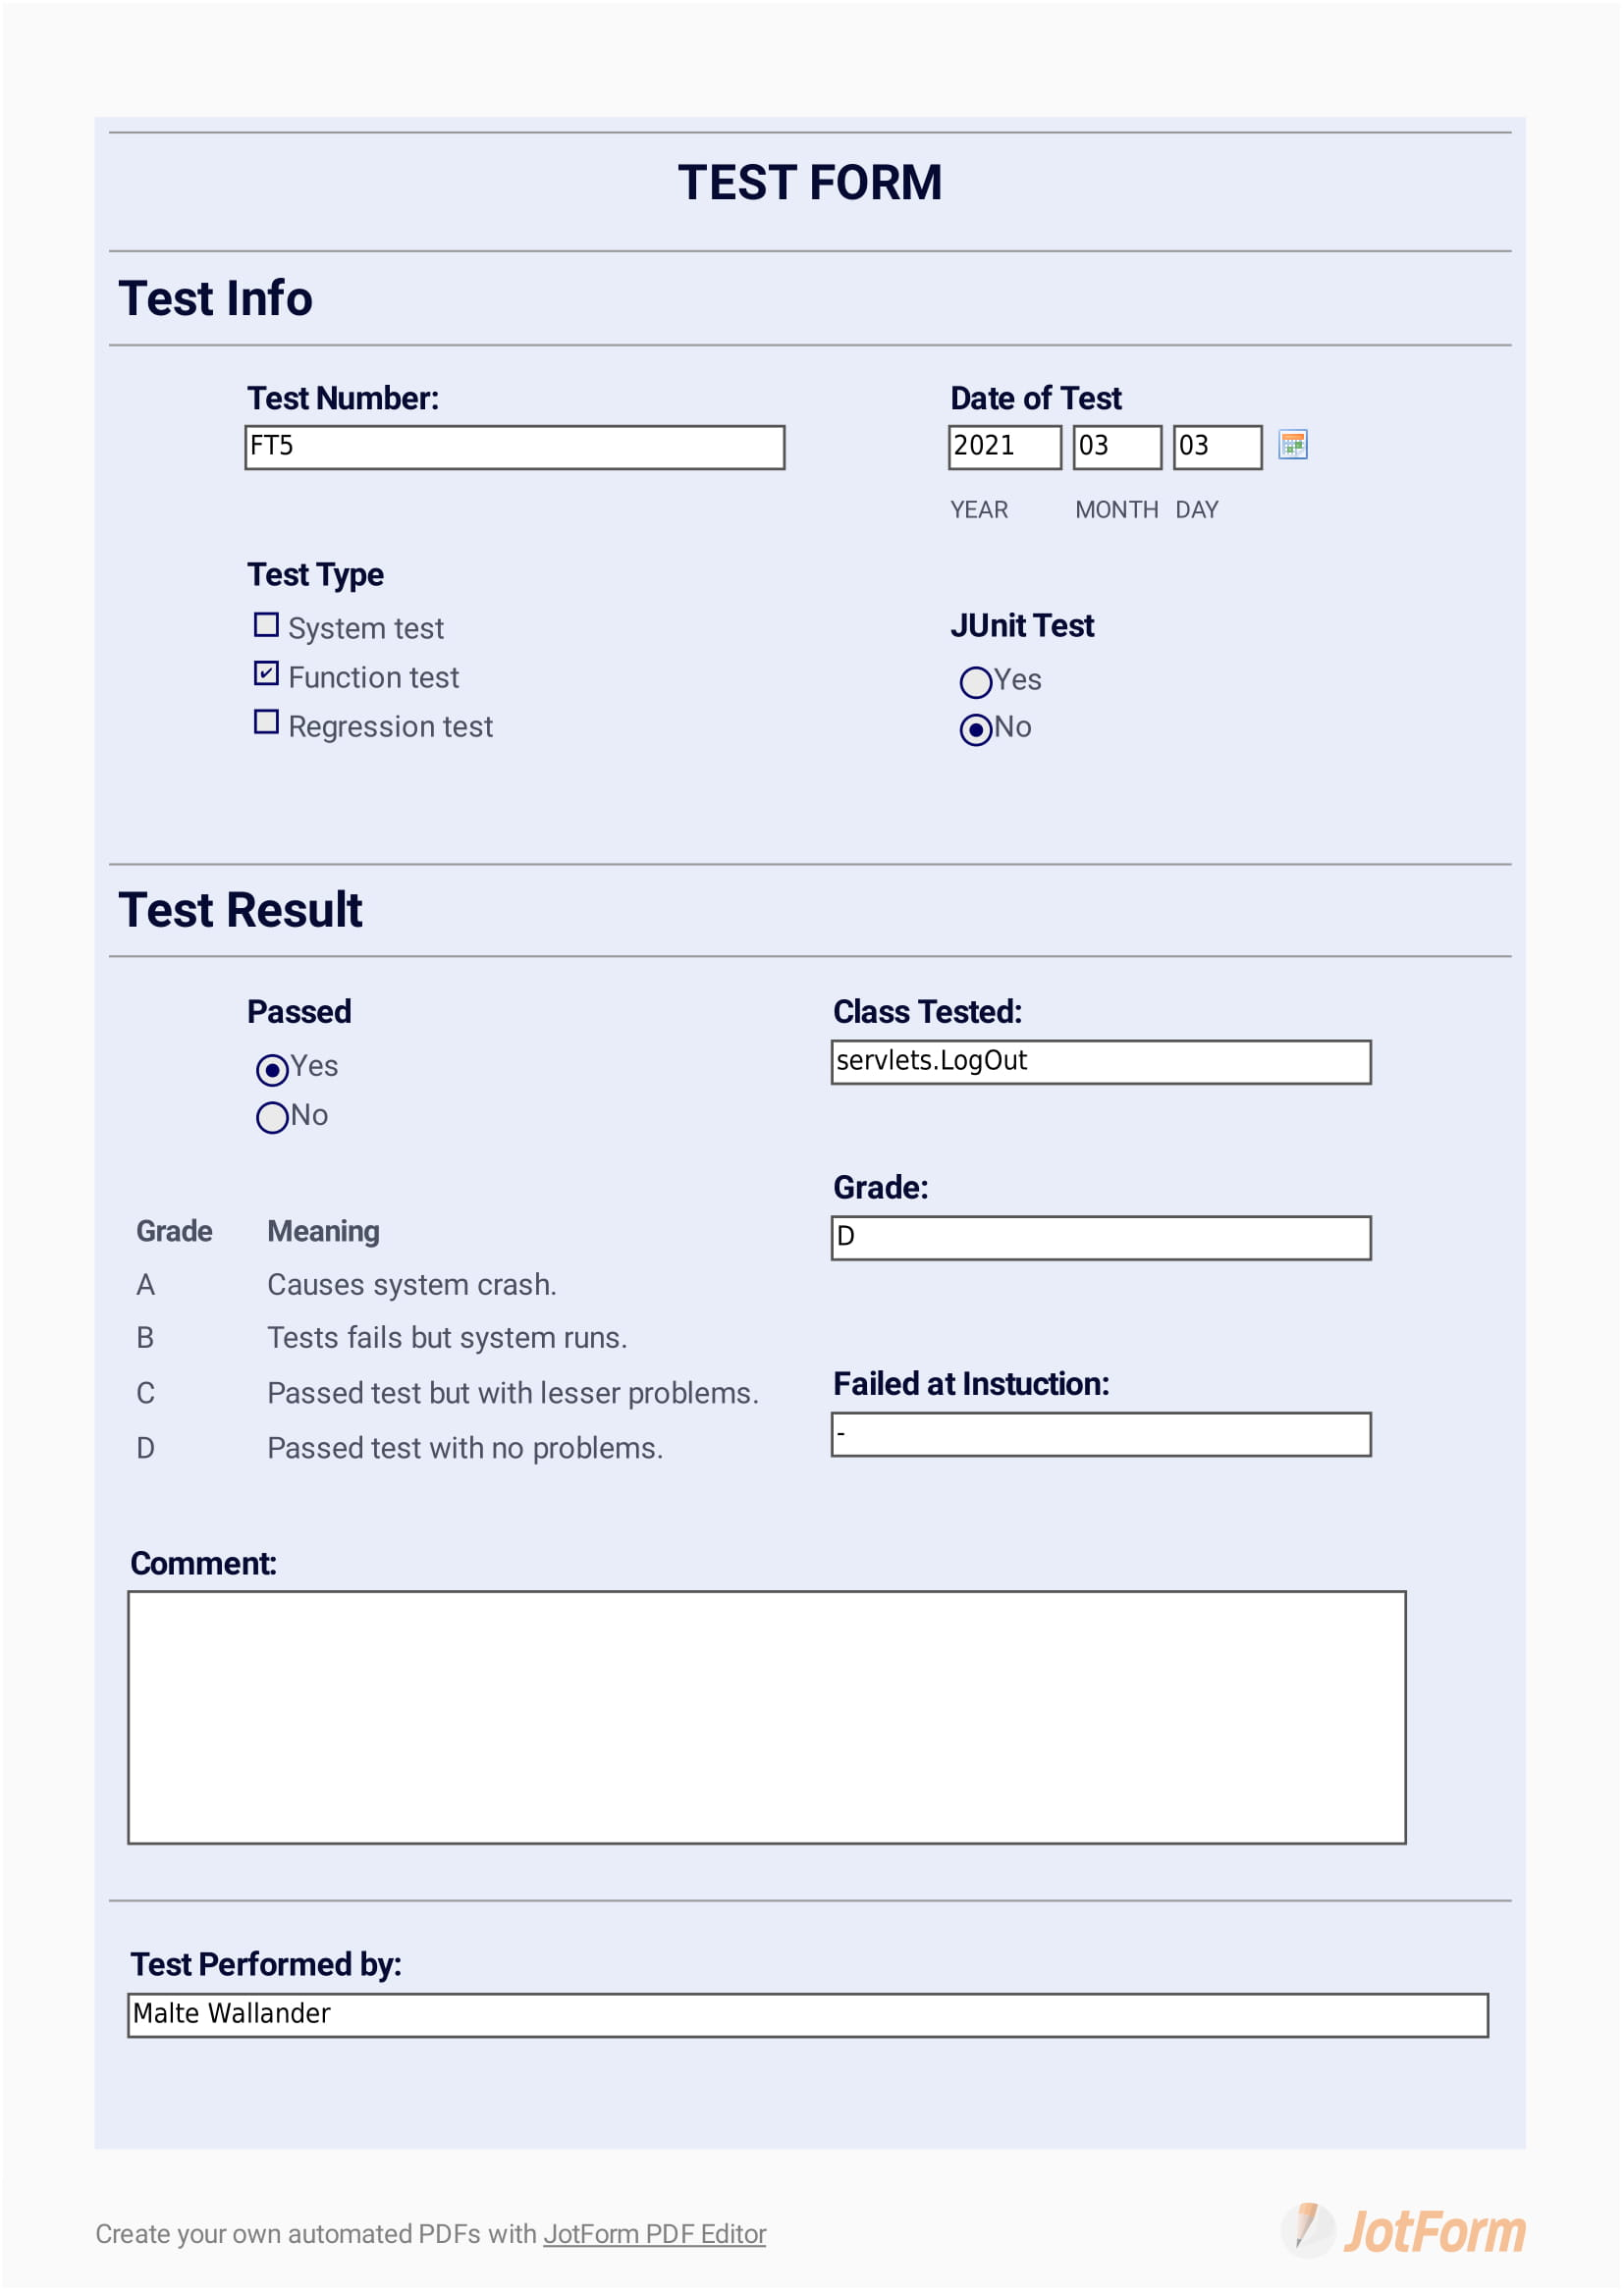
\includegraphics[width=13cm]{images/2021-03-03_Malte_FT5-1}
     \renewcommand\figurename{Figure}
     \caption{Test form for FT5}
     \label{fig:my_label}
 \end{figure}
 
 \begin{figure}
     \centering
     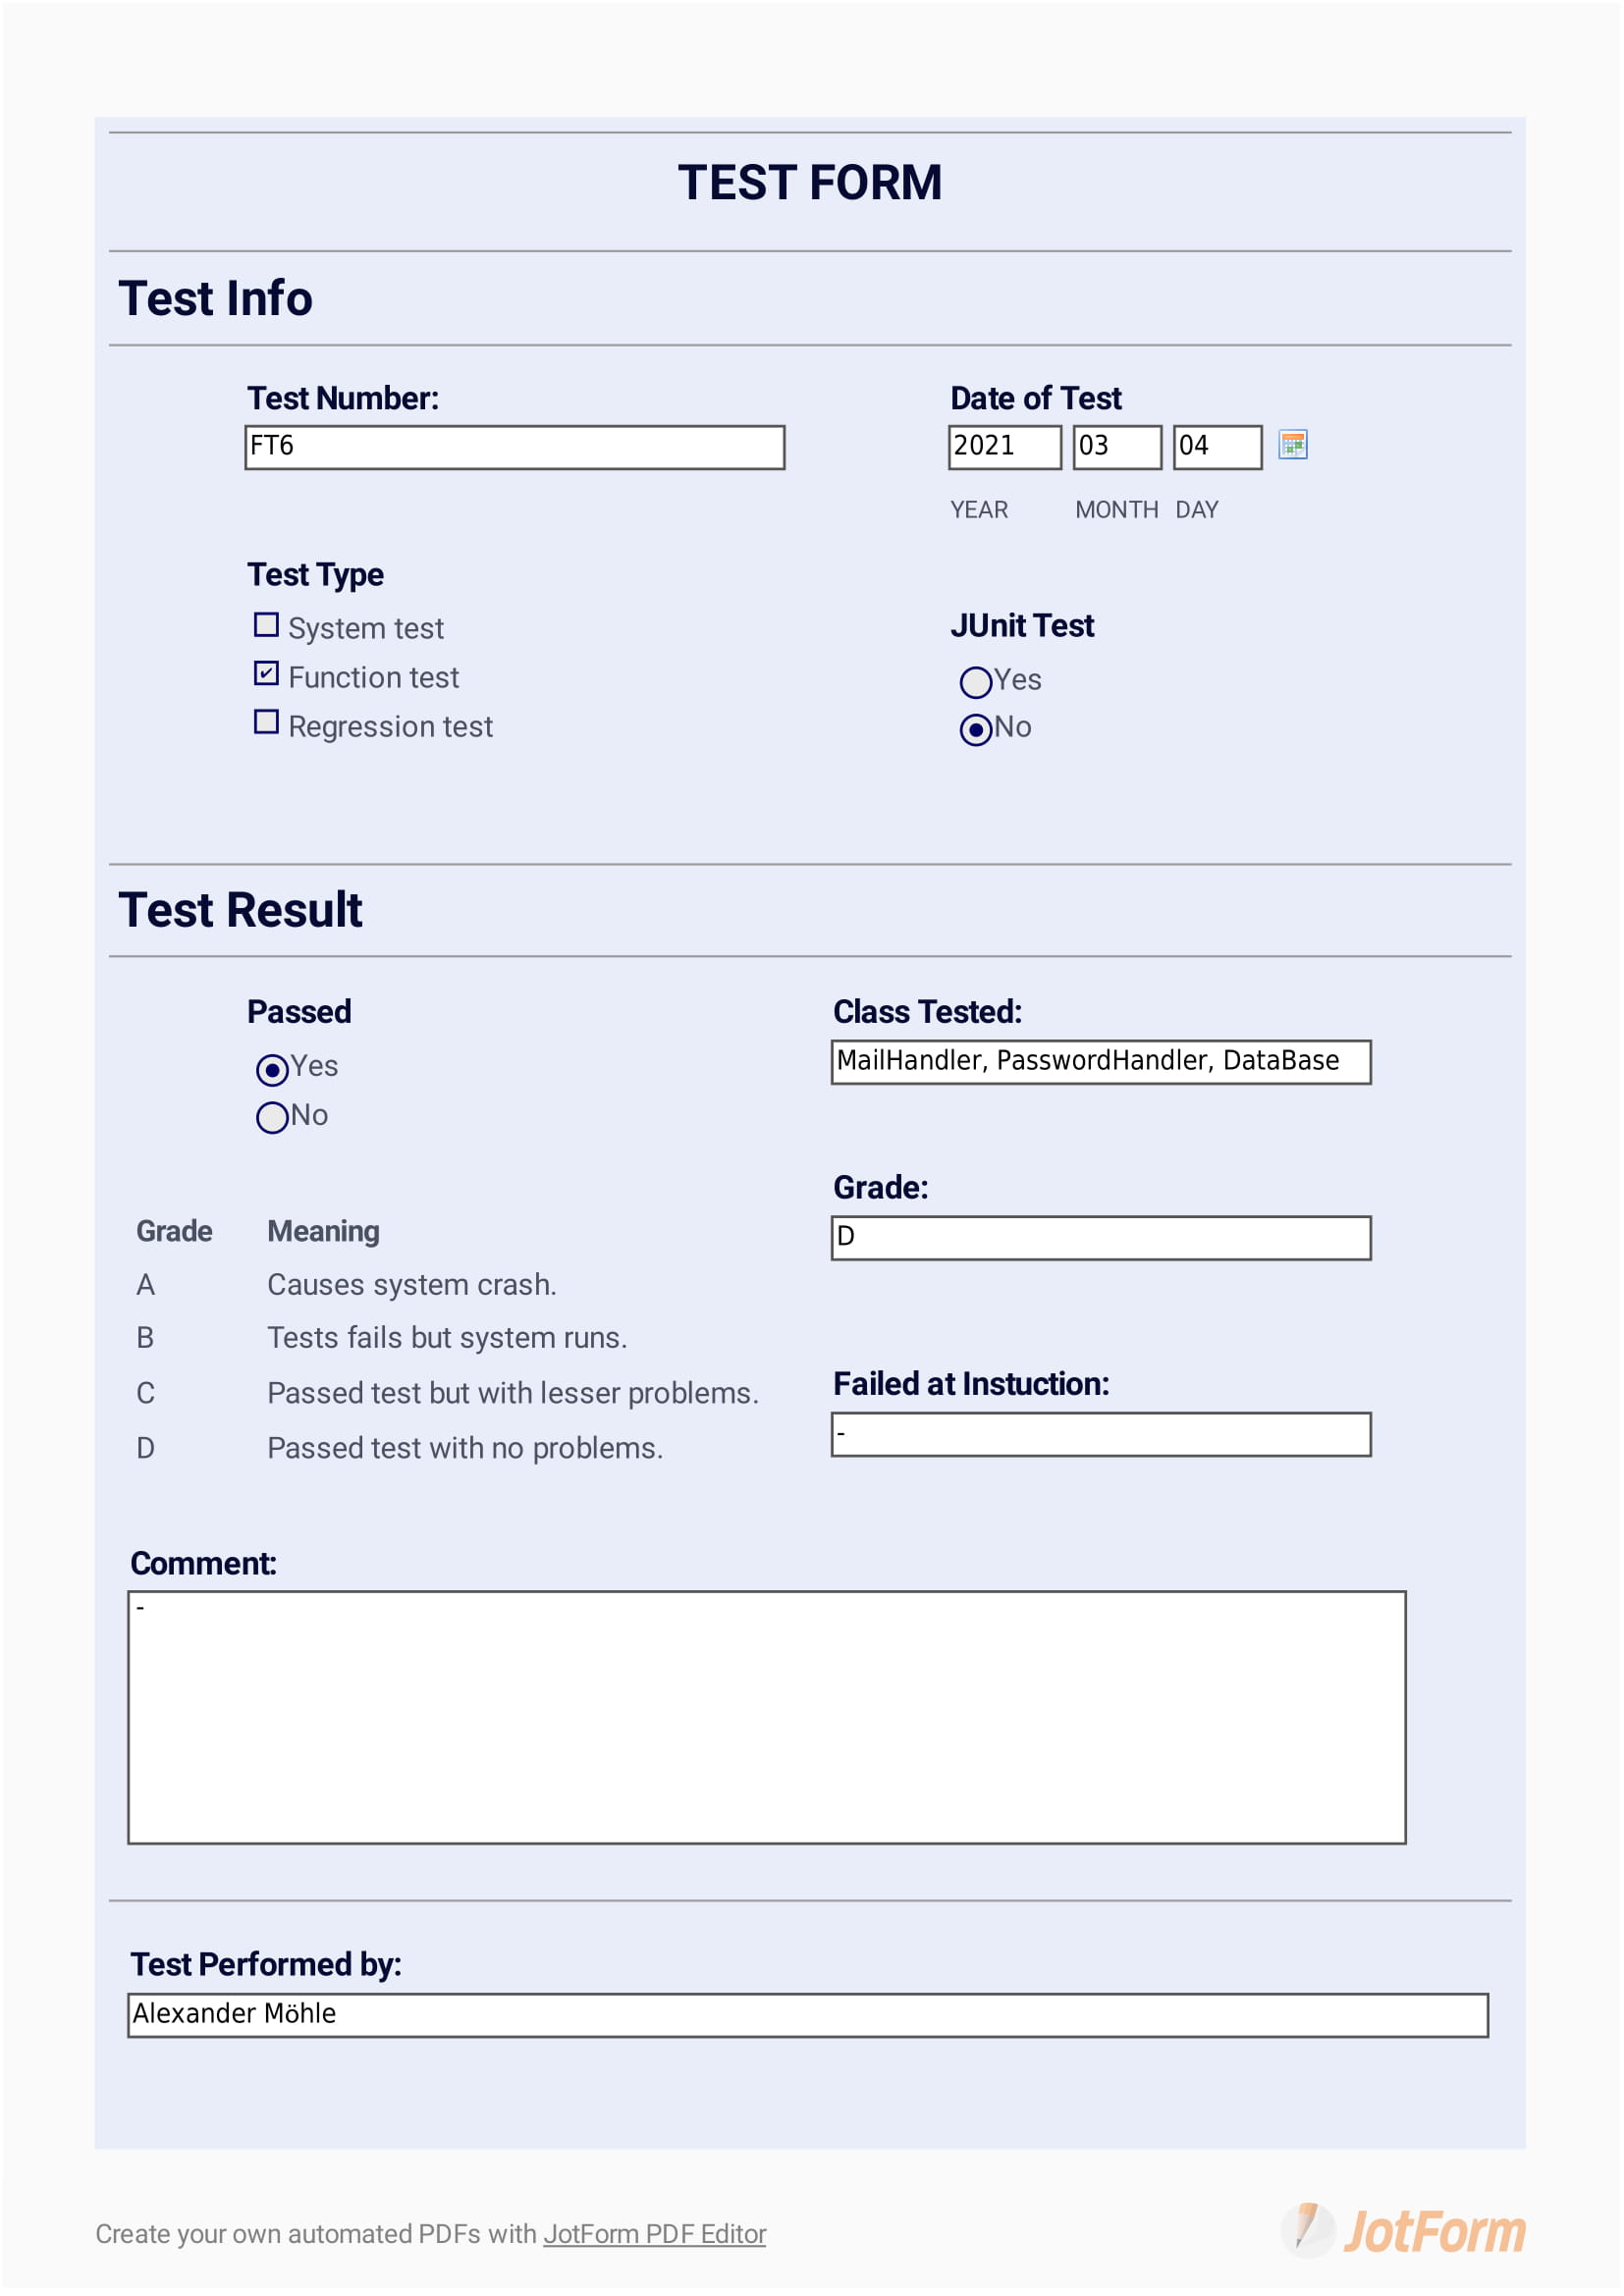
\includegraphics[width=13cm]{images/2021-03-04_Alexander_FT6-1}
     \renewcommand\figurename{Figure}
     \caption{Test form for FT6}
     \label{fig:my_label}
 \end{figure}
 
 \begin{figure}
     \centering
     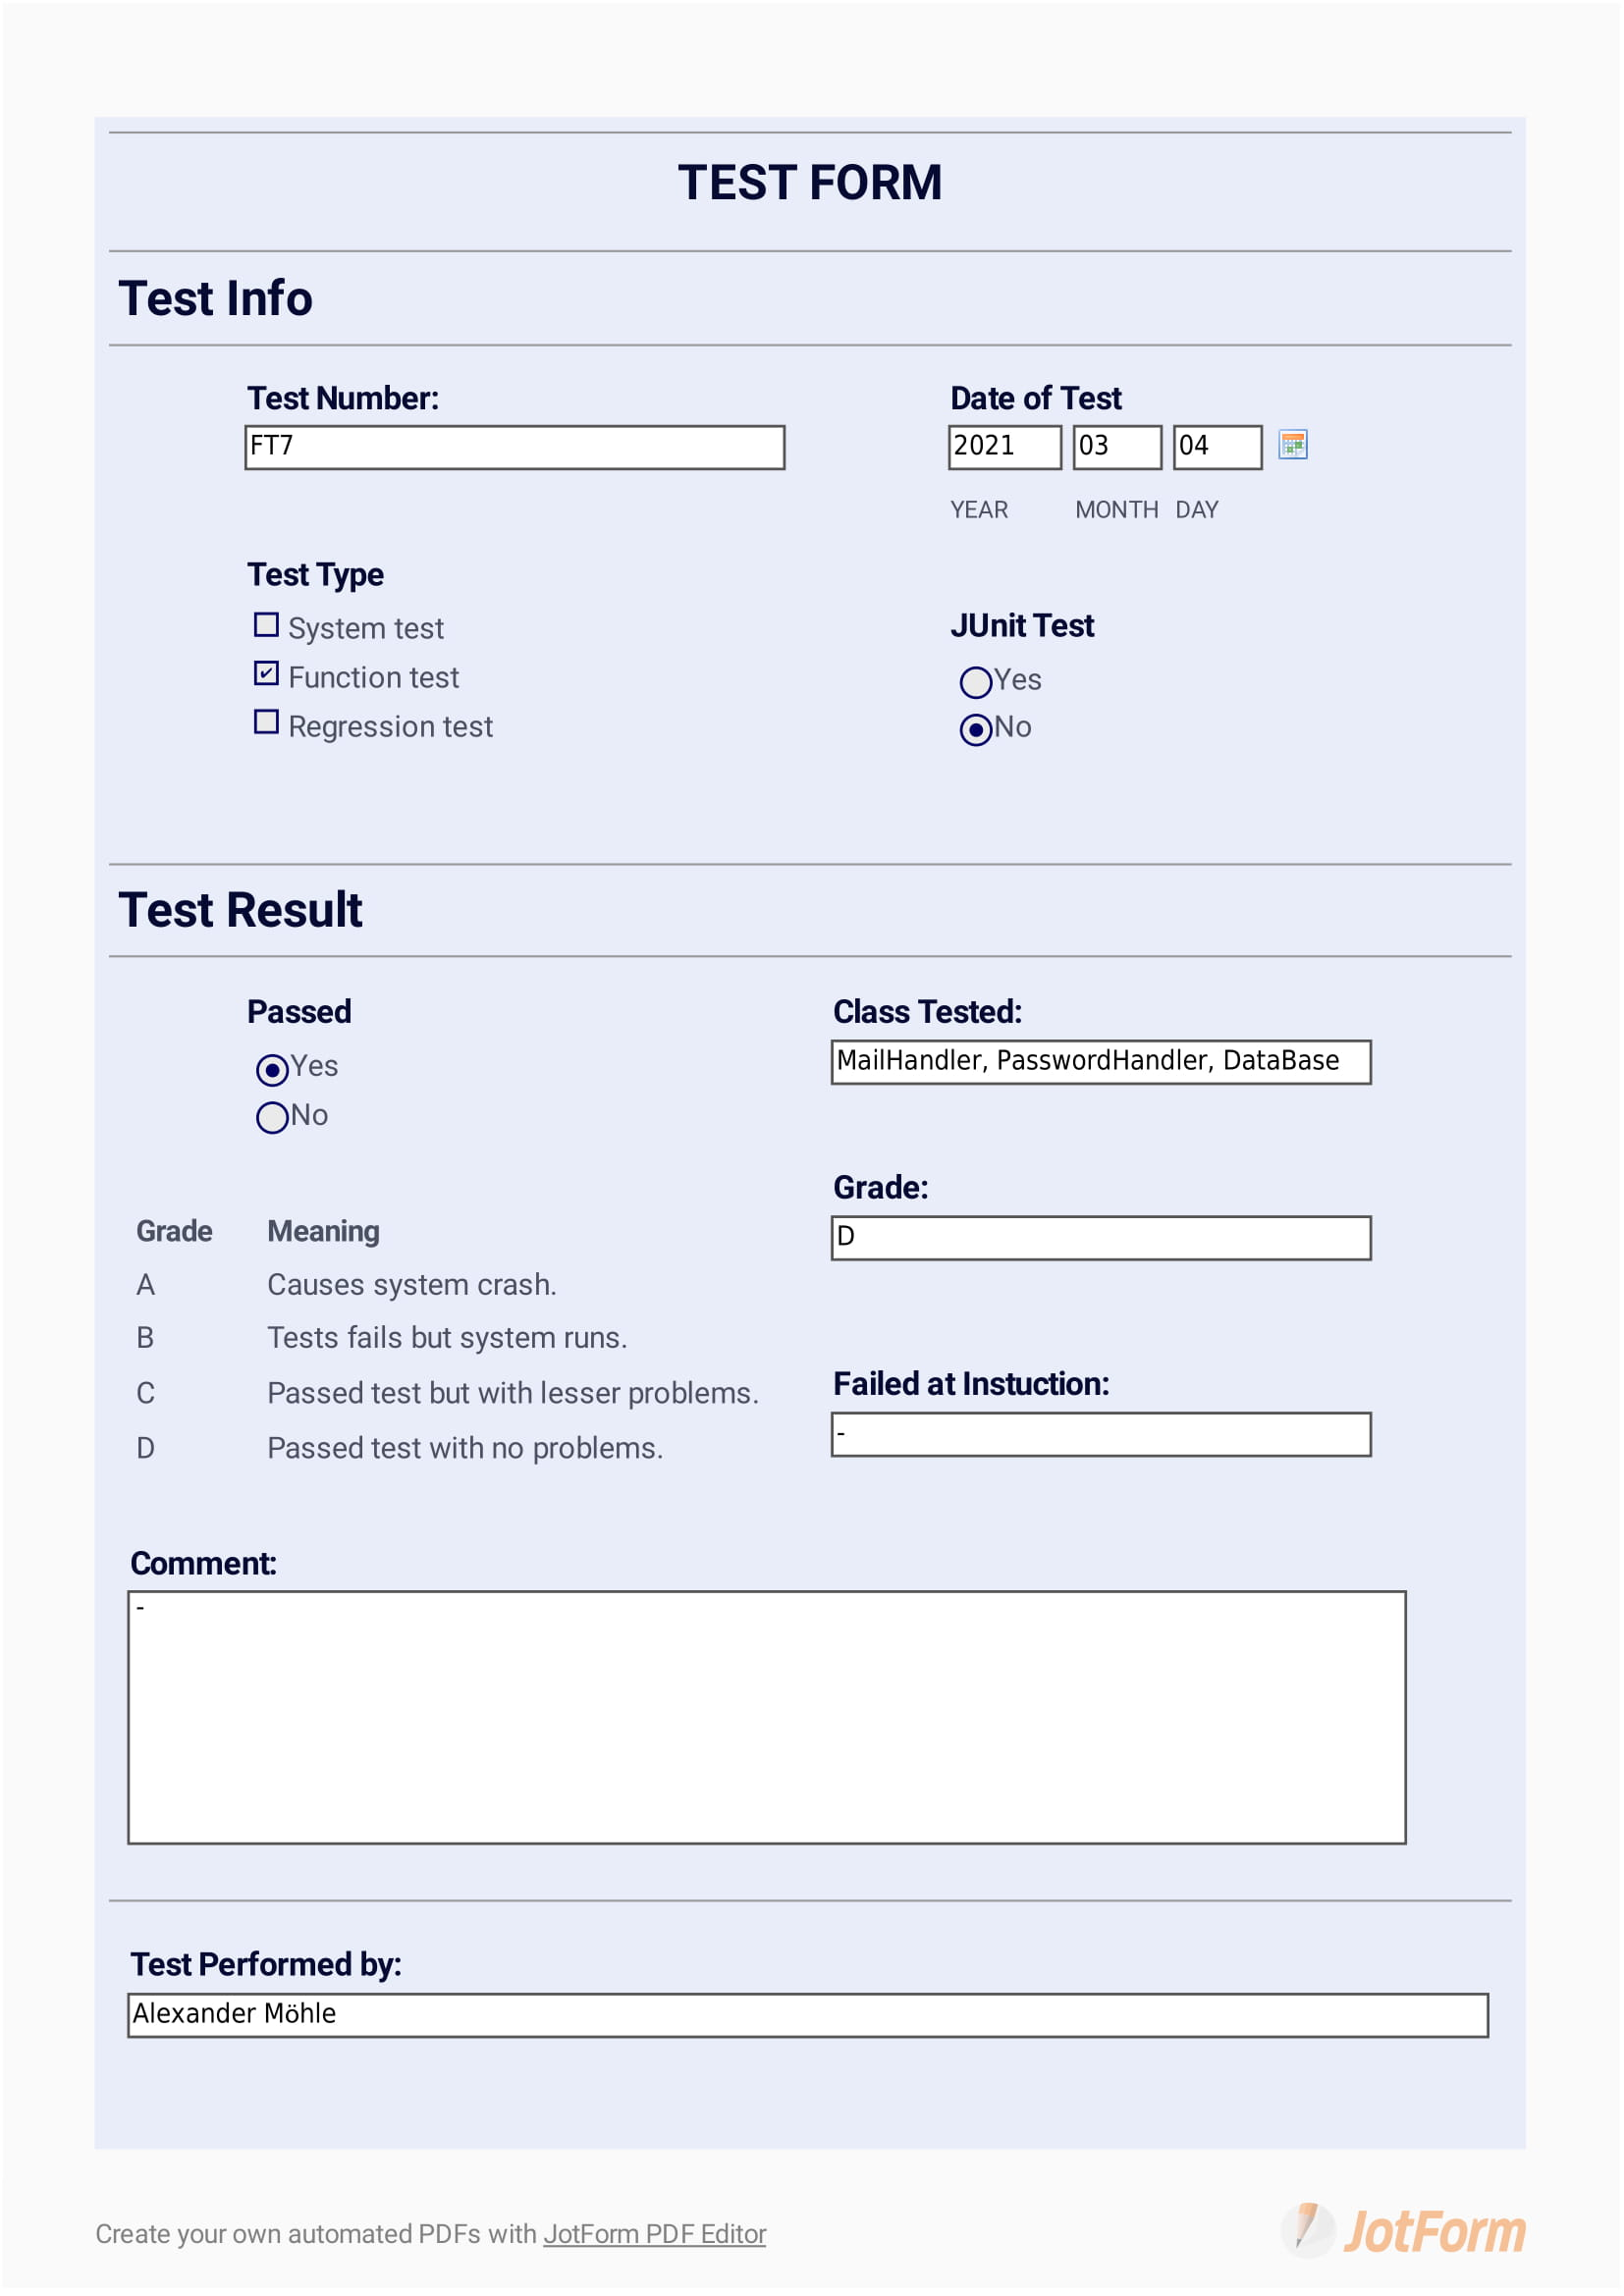
\includegraphics[width=13cm]{images/2021-03-04_Alexander_FT7-1}
     \renewcommand\figurename{Figure}
     \caption{Test form for FT7}
     \label{fig:my_label}
 \end{figure}
 
 \begin{figure}
     \centering
     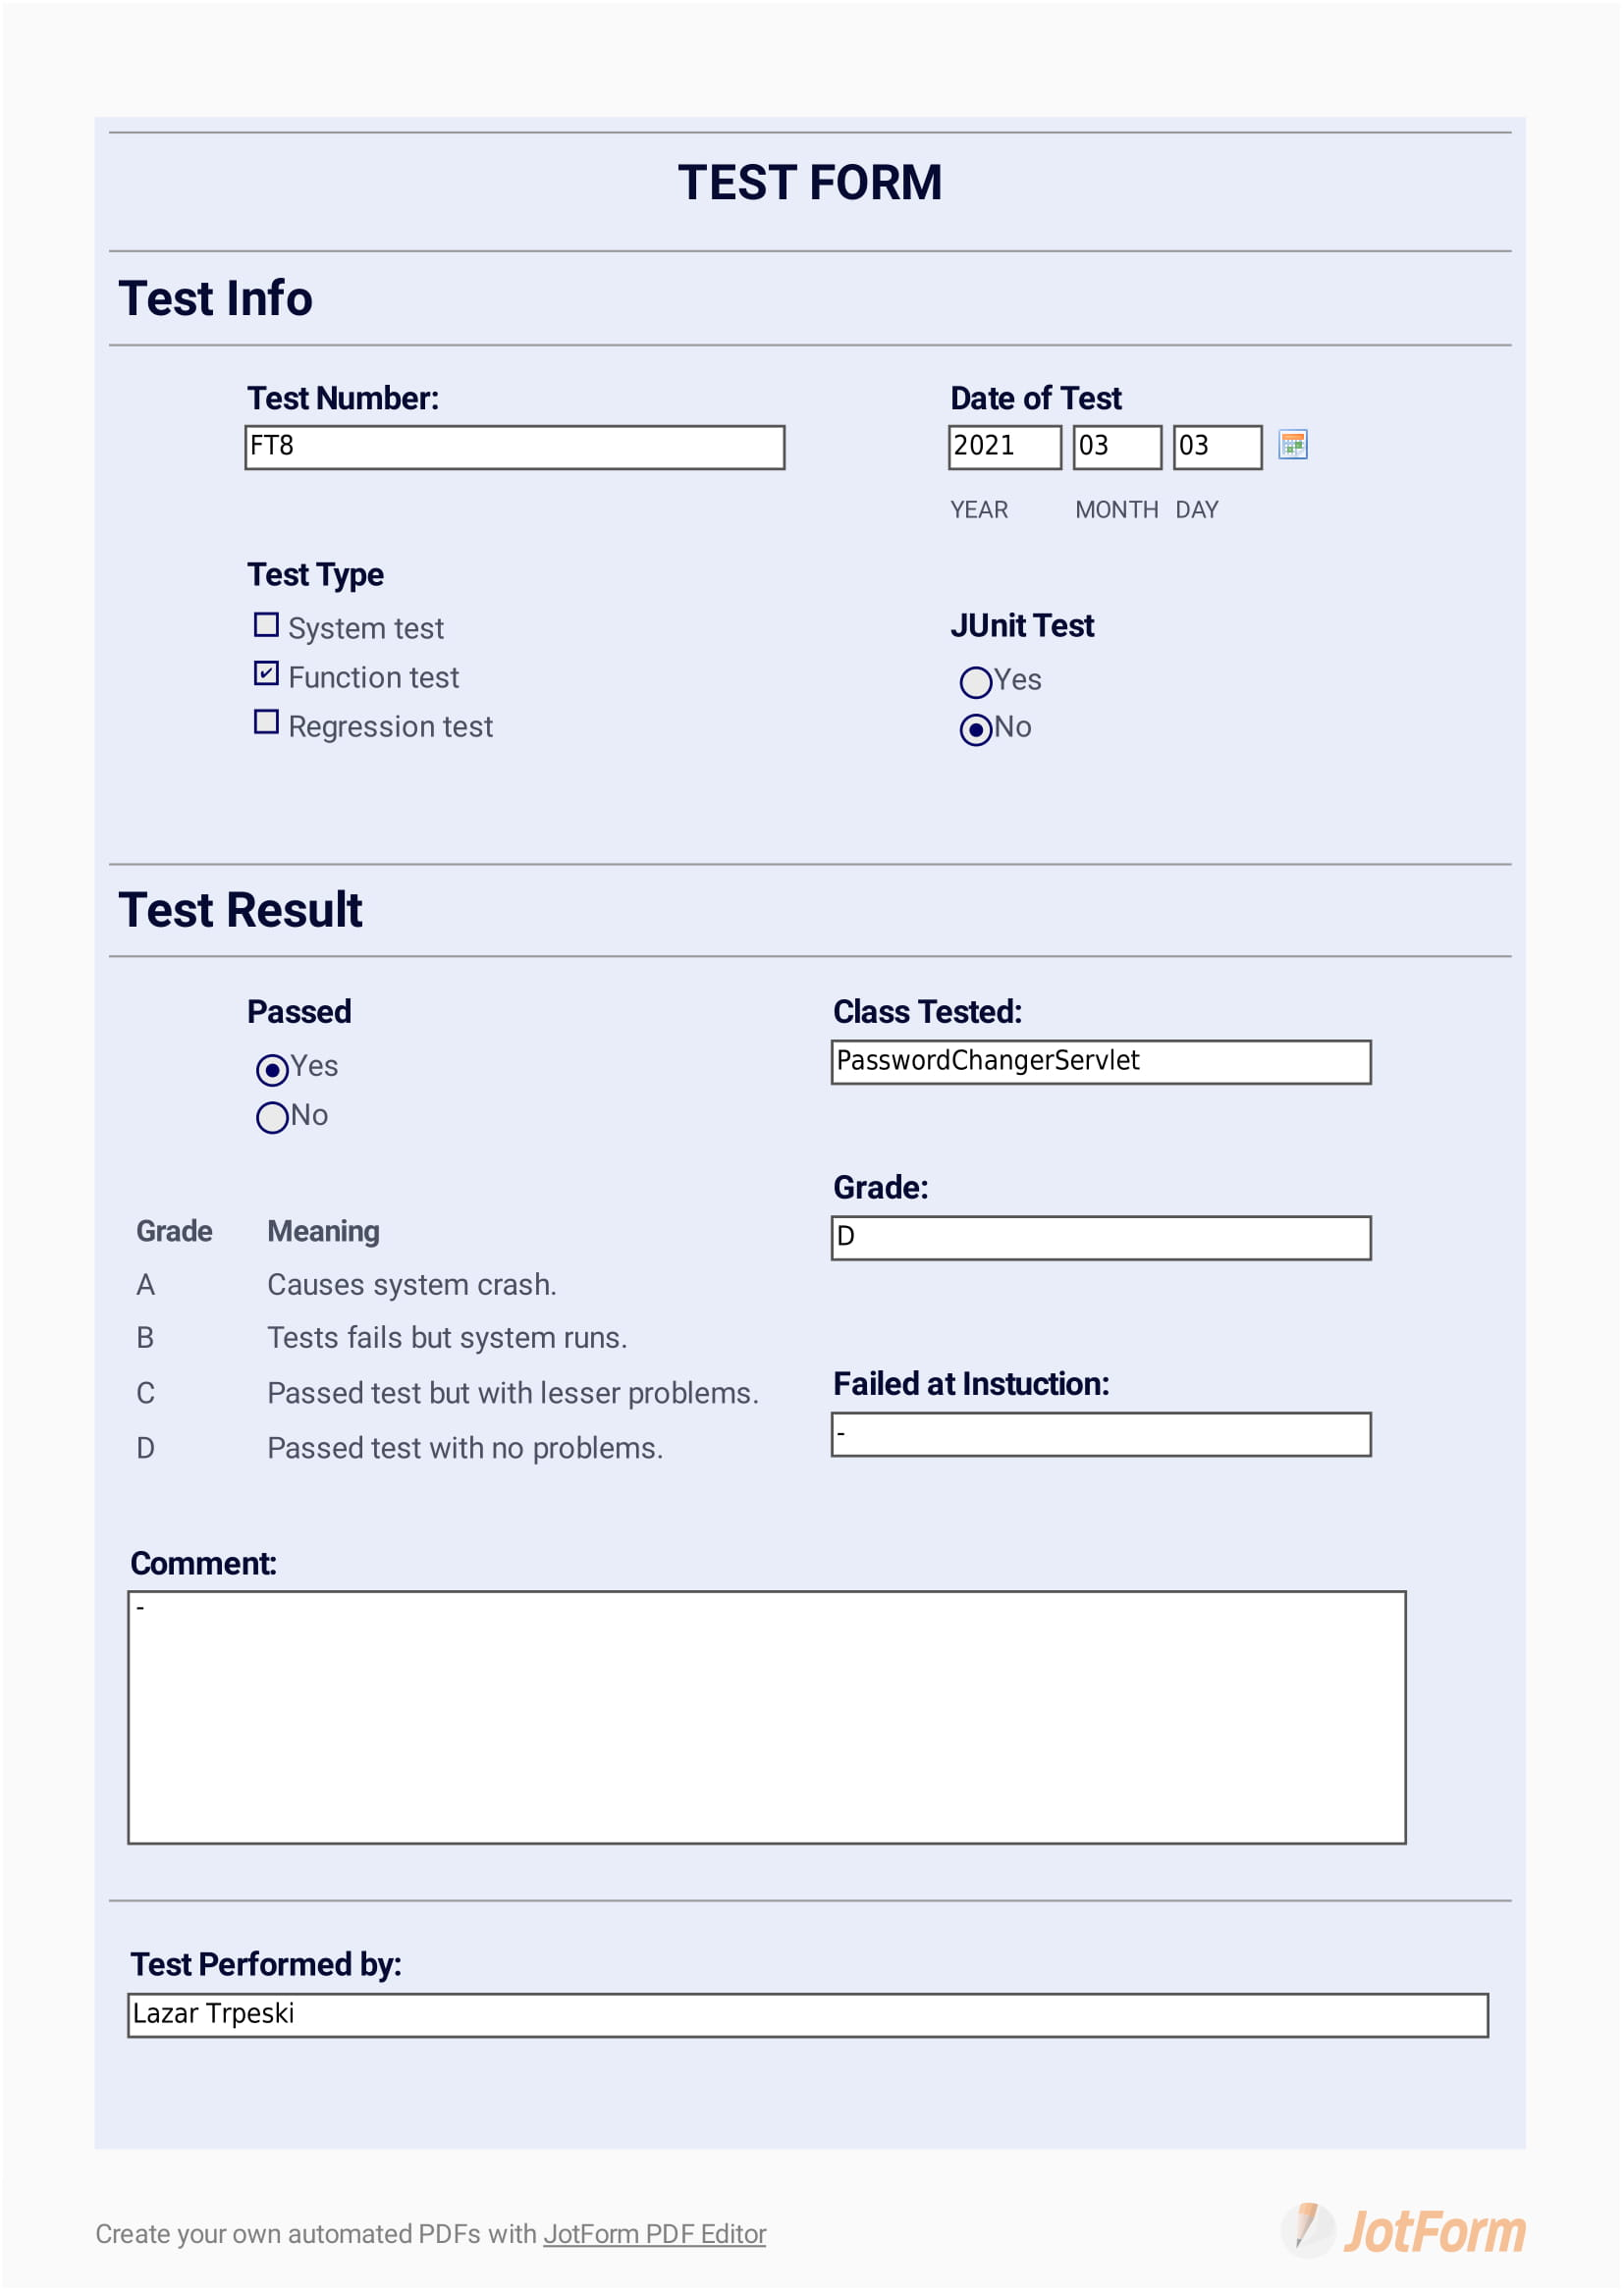
\includegraphics[width=13cm]{images/2021-03-03_Lazar_FT8-1}
     \renewcommand\figurename{Figure}
     \caption{Test form for FT8}
     \label{fig:my_label}
 \end{figure}
 
 \begin{figure}
     \centering
     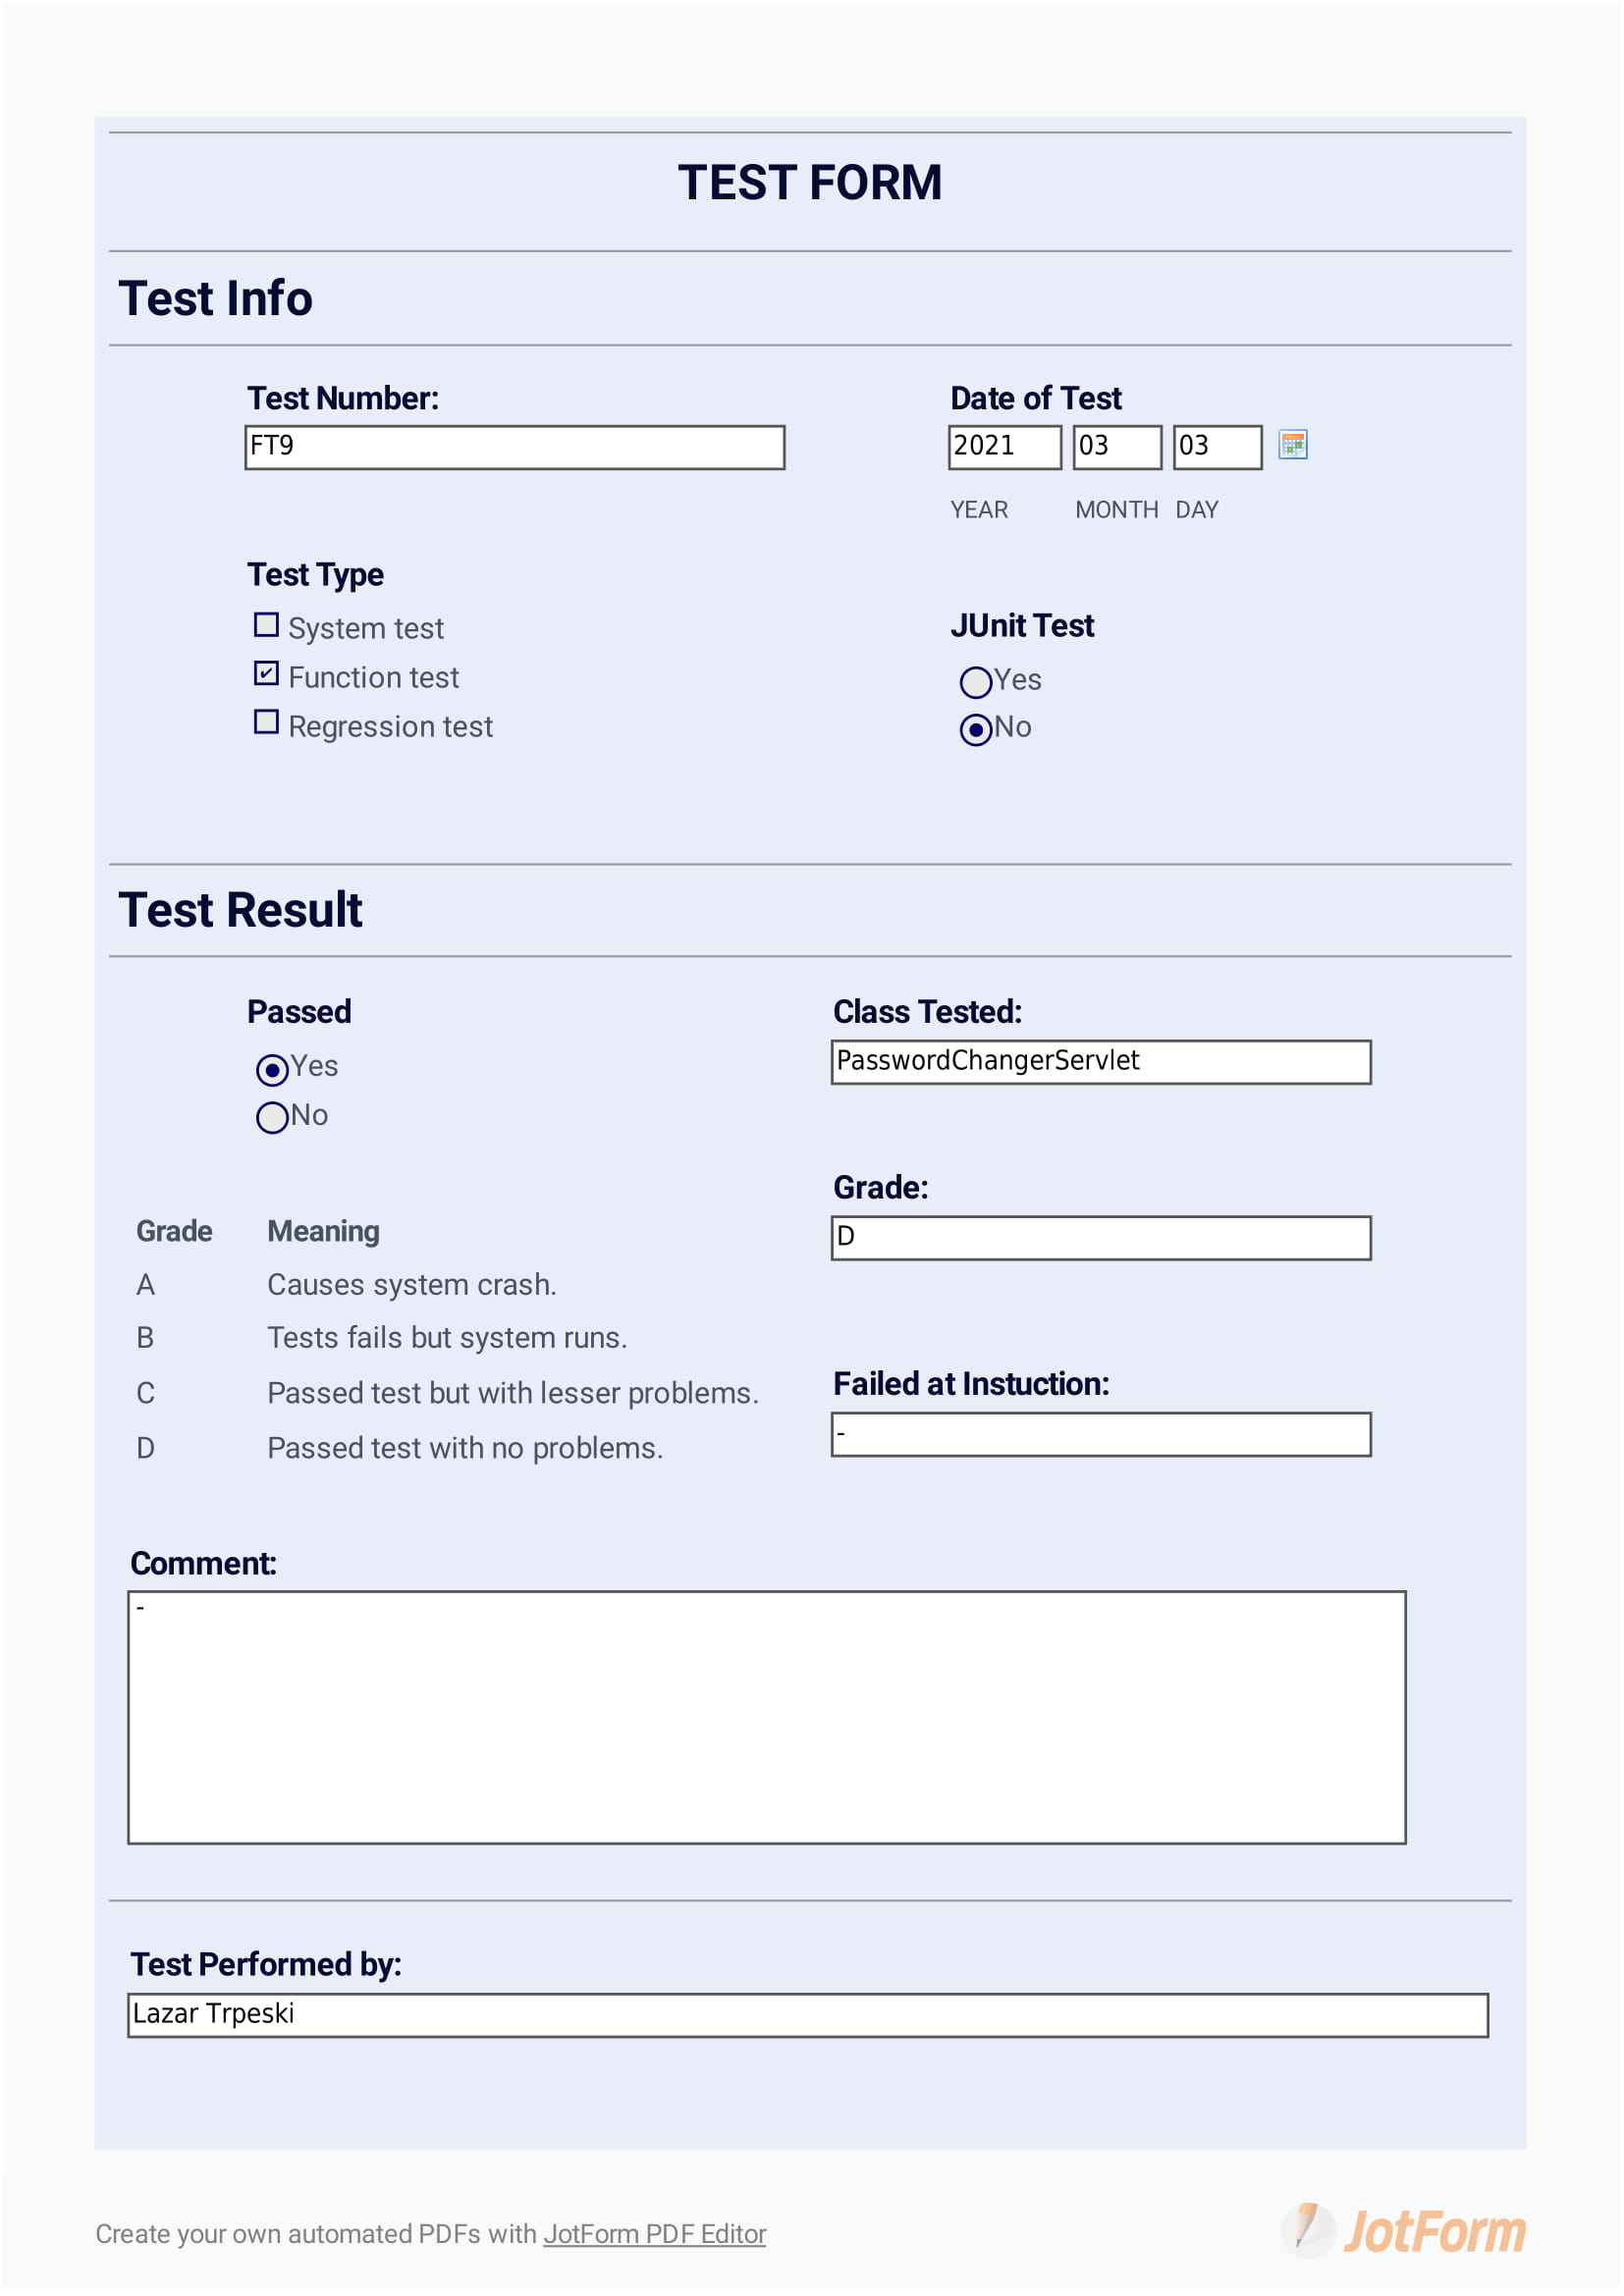
\includegraphics[width=13cm]{images/2021-03-03_Lazar_FT9-1}
     \renewcommand\figurename{Figure}
     \caption{Test form for FT9}
     \label{fig:my_label}
 \end{figure}
 
 \begin{figure}
     \centering
     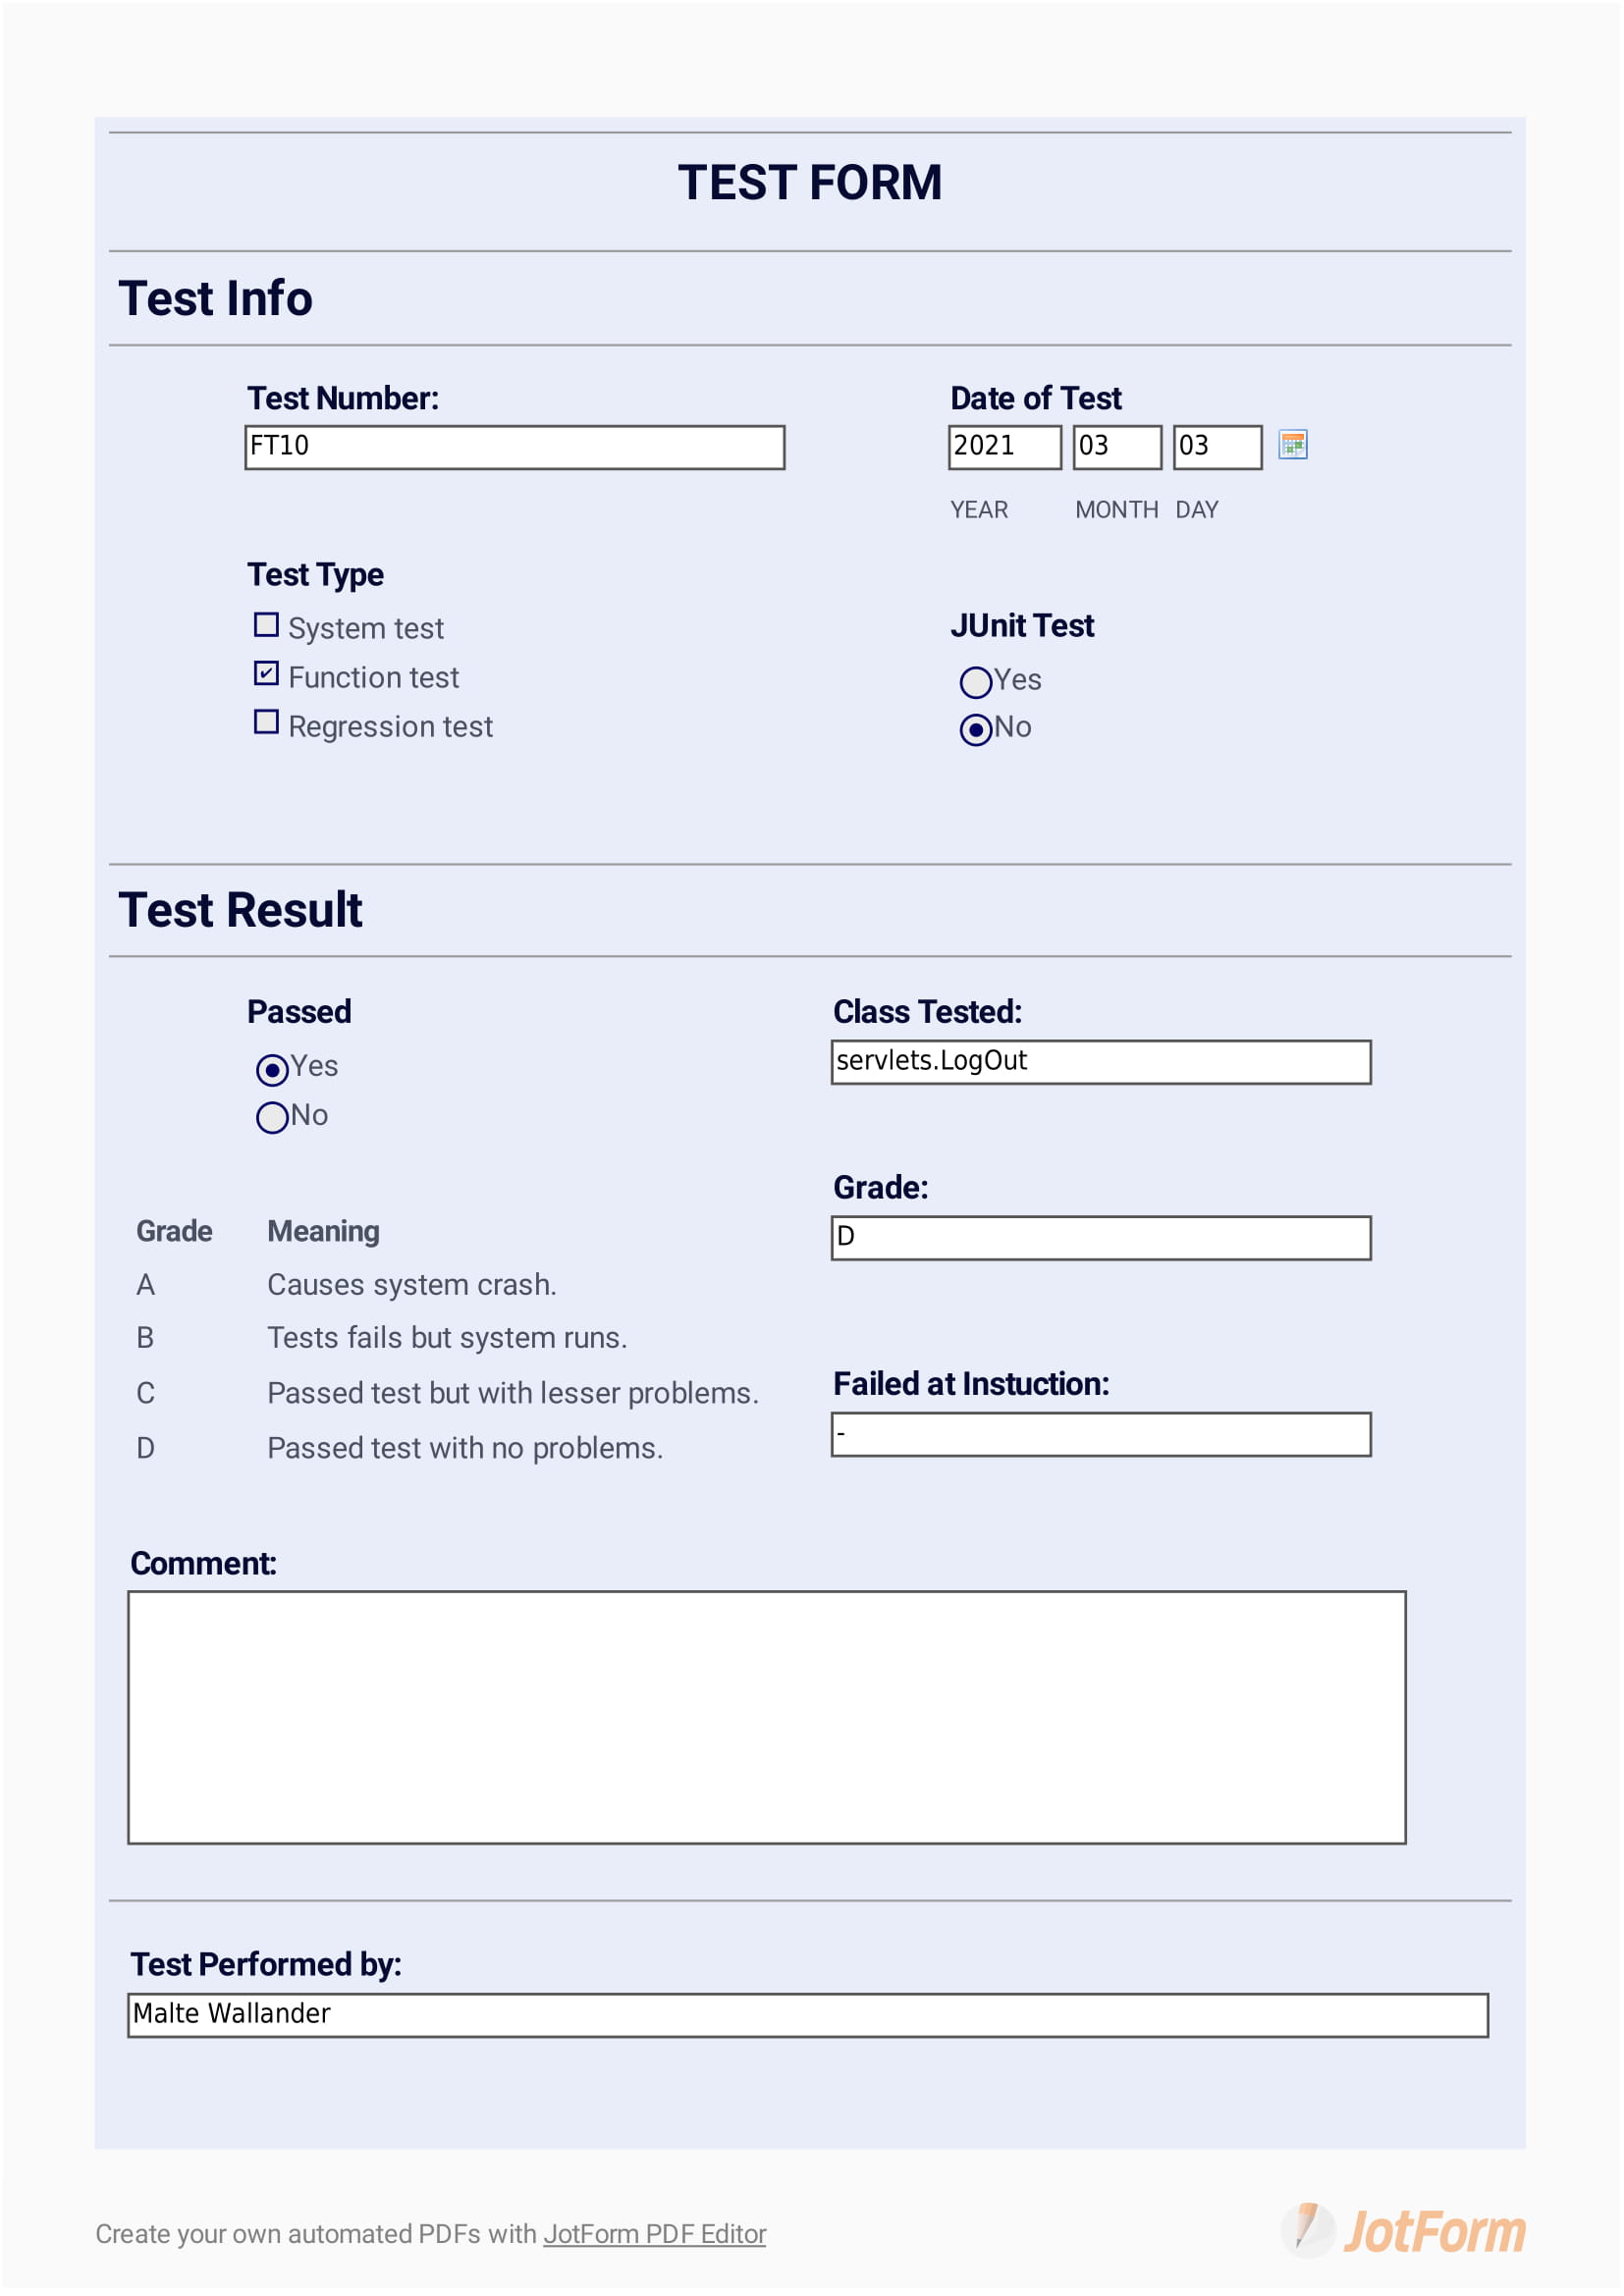
\includegraphics[width=13cm]{images/2021-03-03_Malte_FT10-1}
     \renewcommand\figurename{Figure}
     \caption{Test form for FT10}
     \label{fig:my_label}
 \end{figure}
 
 \begin{figure}
     \centering
     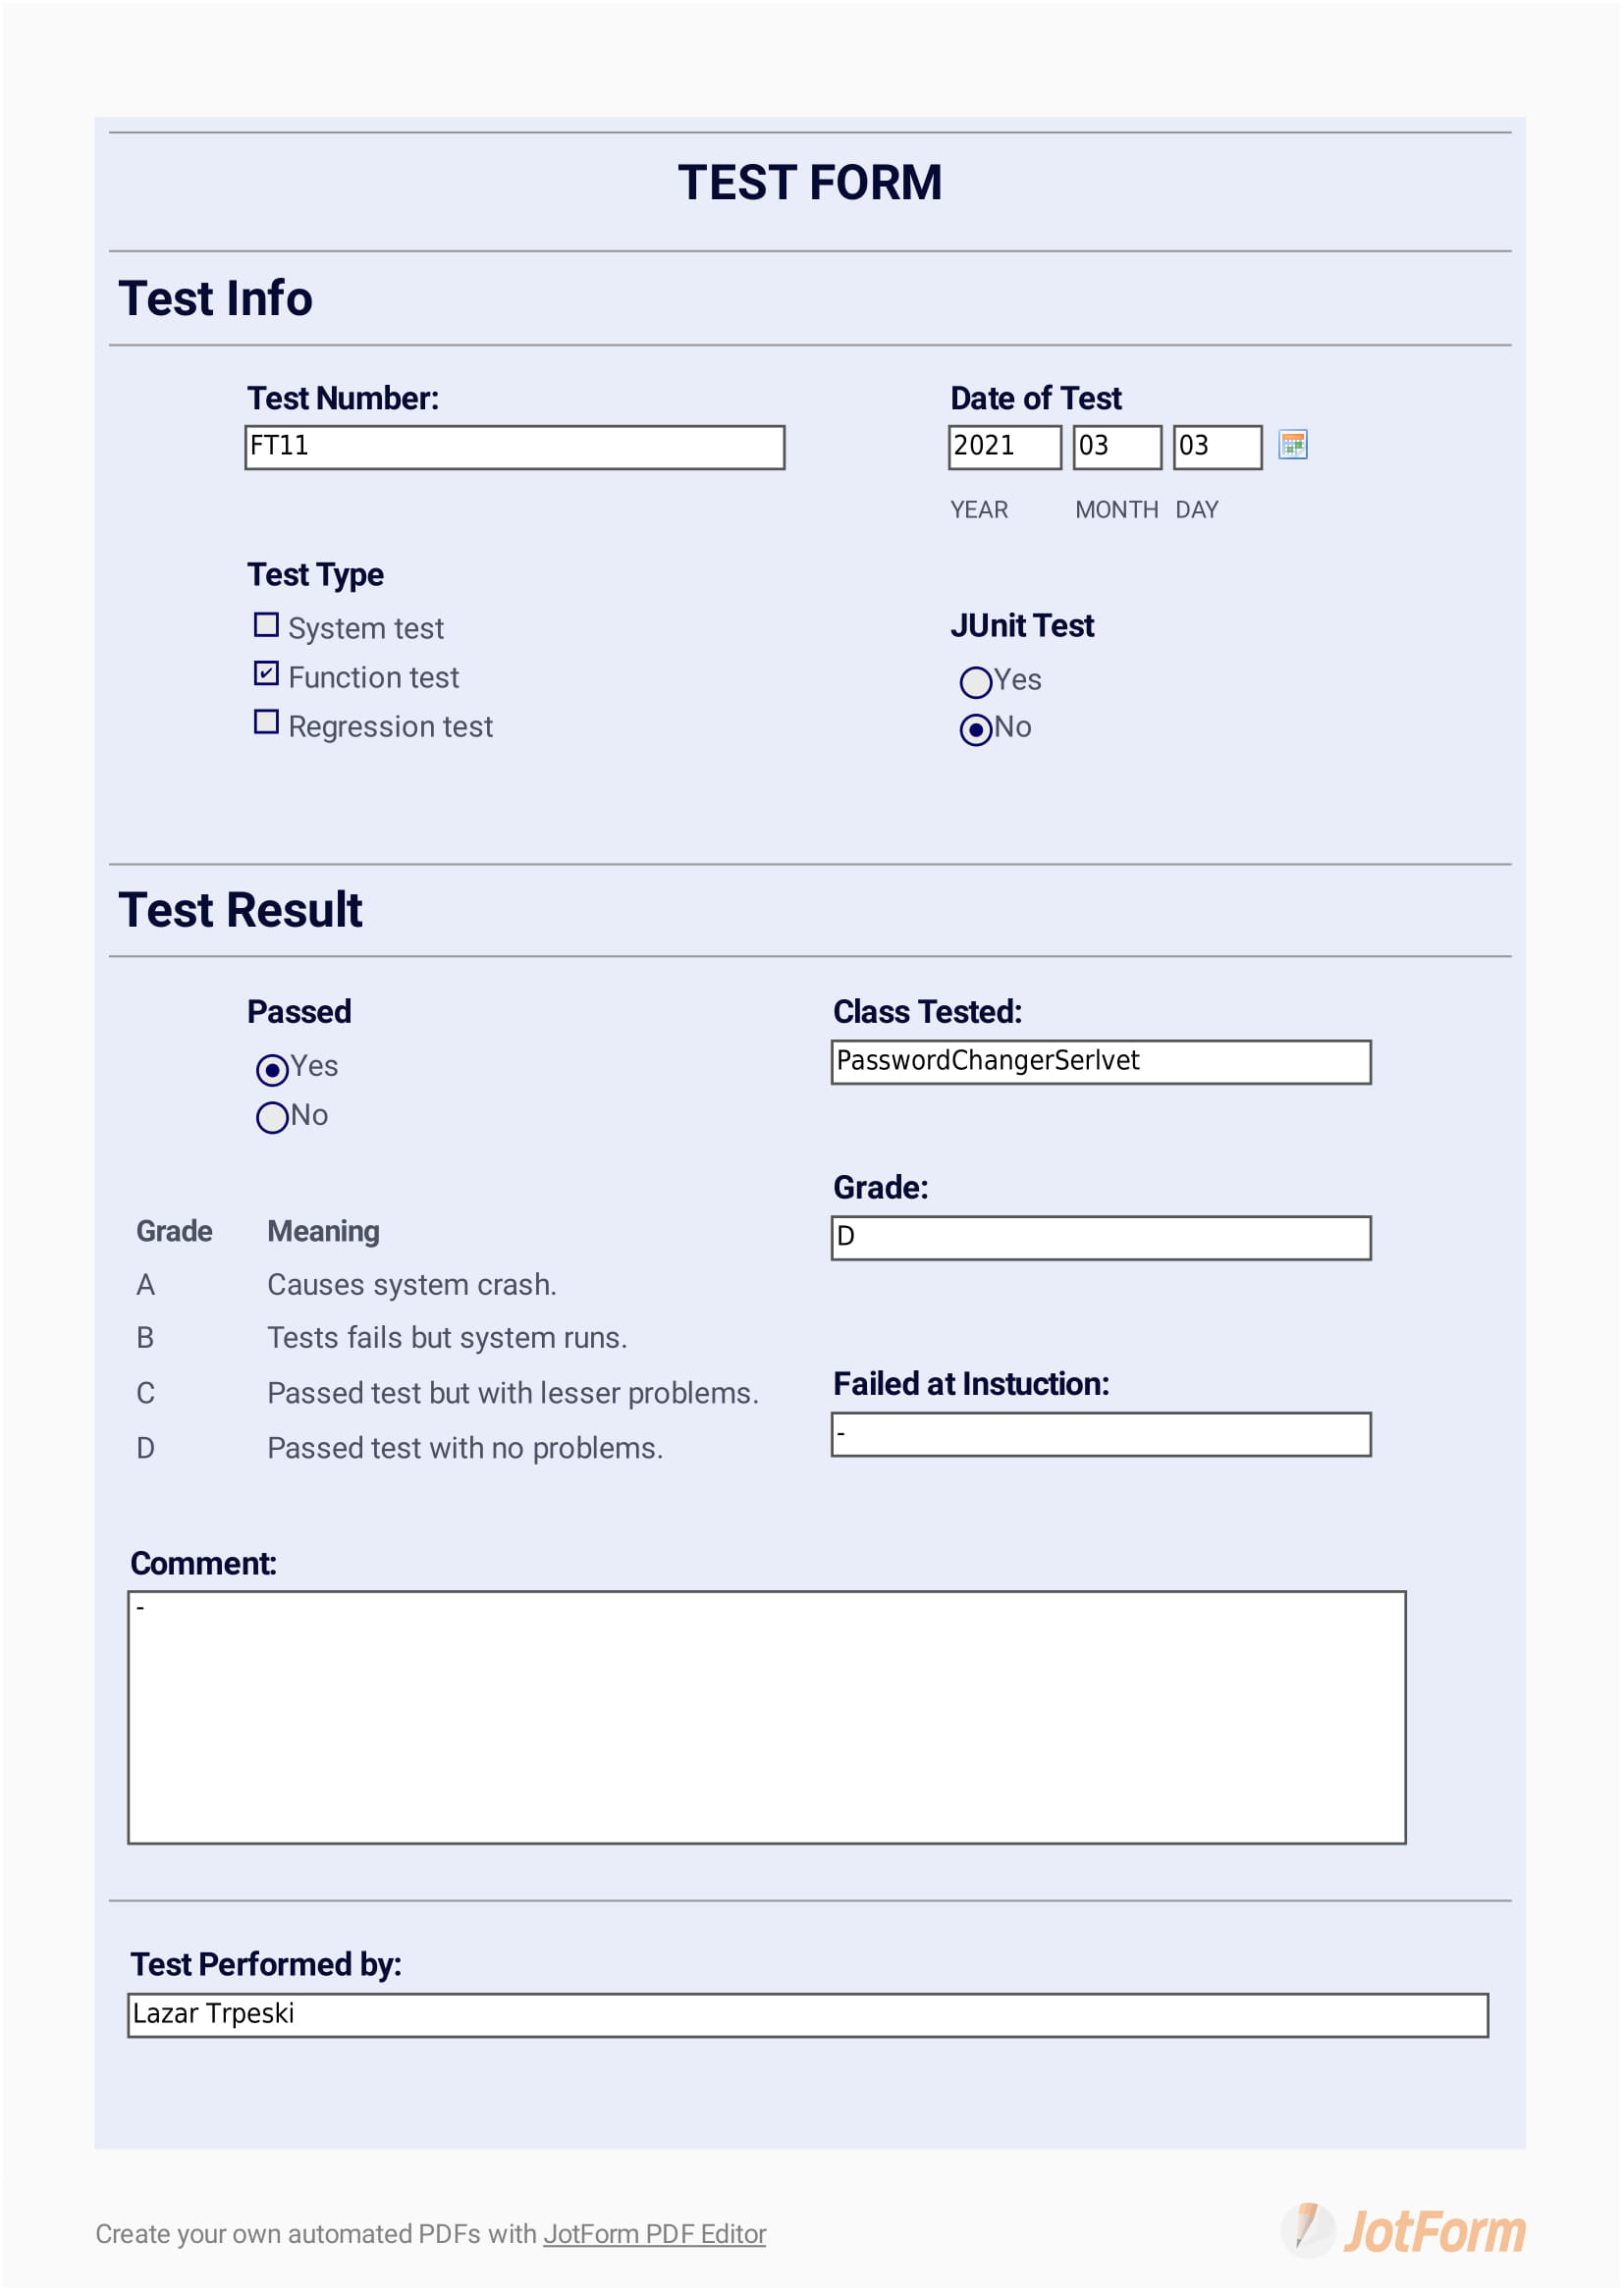
\includegraphics[width=13cm]{images/2021-03-03_Lazar_FT11-1}
     \renewcommand\figurename{Figure}
     \caption{Test form for FT11}
     \label{fig:my_label}
 \end{figure}
 
 \begin{figure}
     \centering
     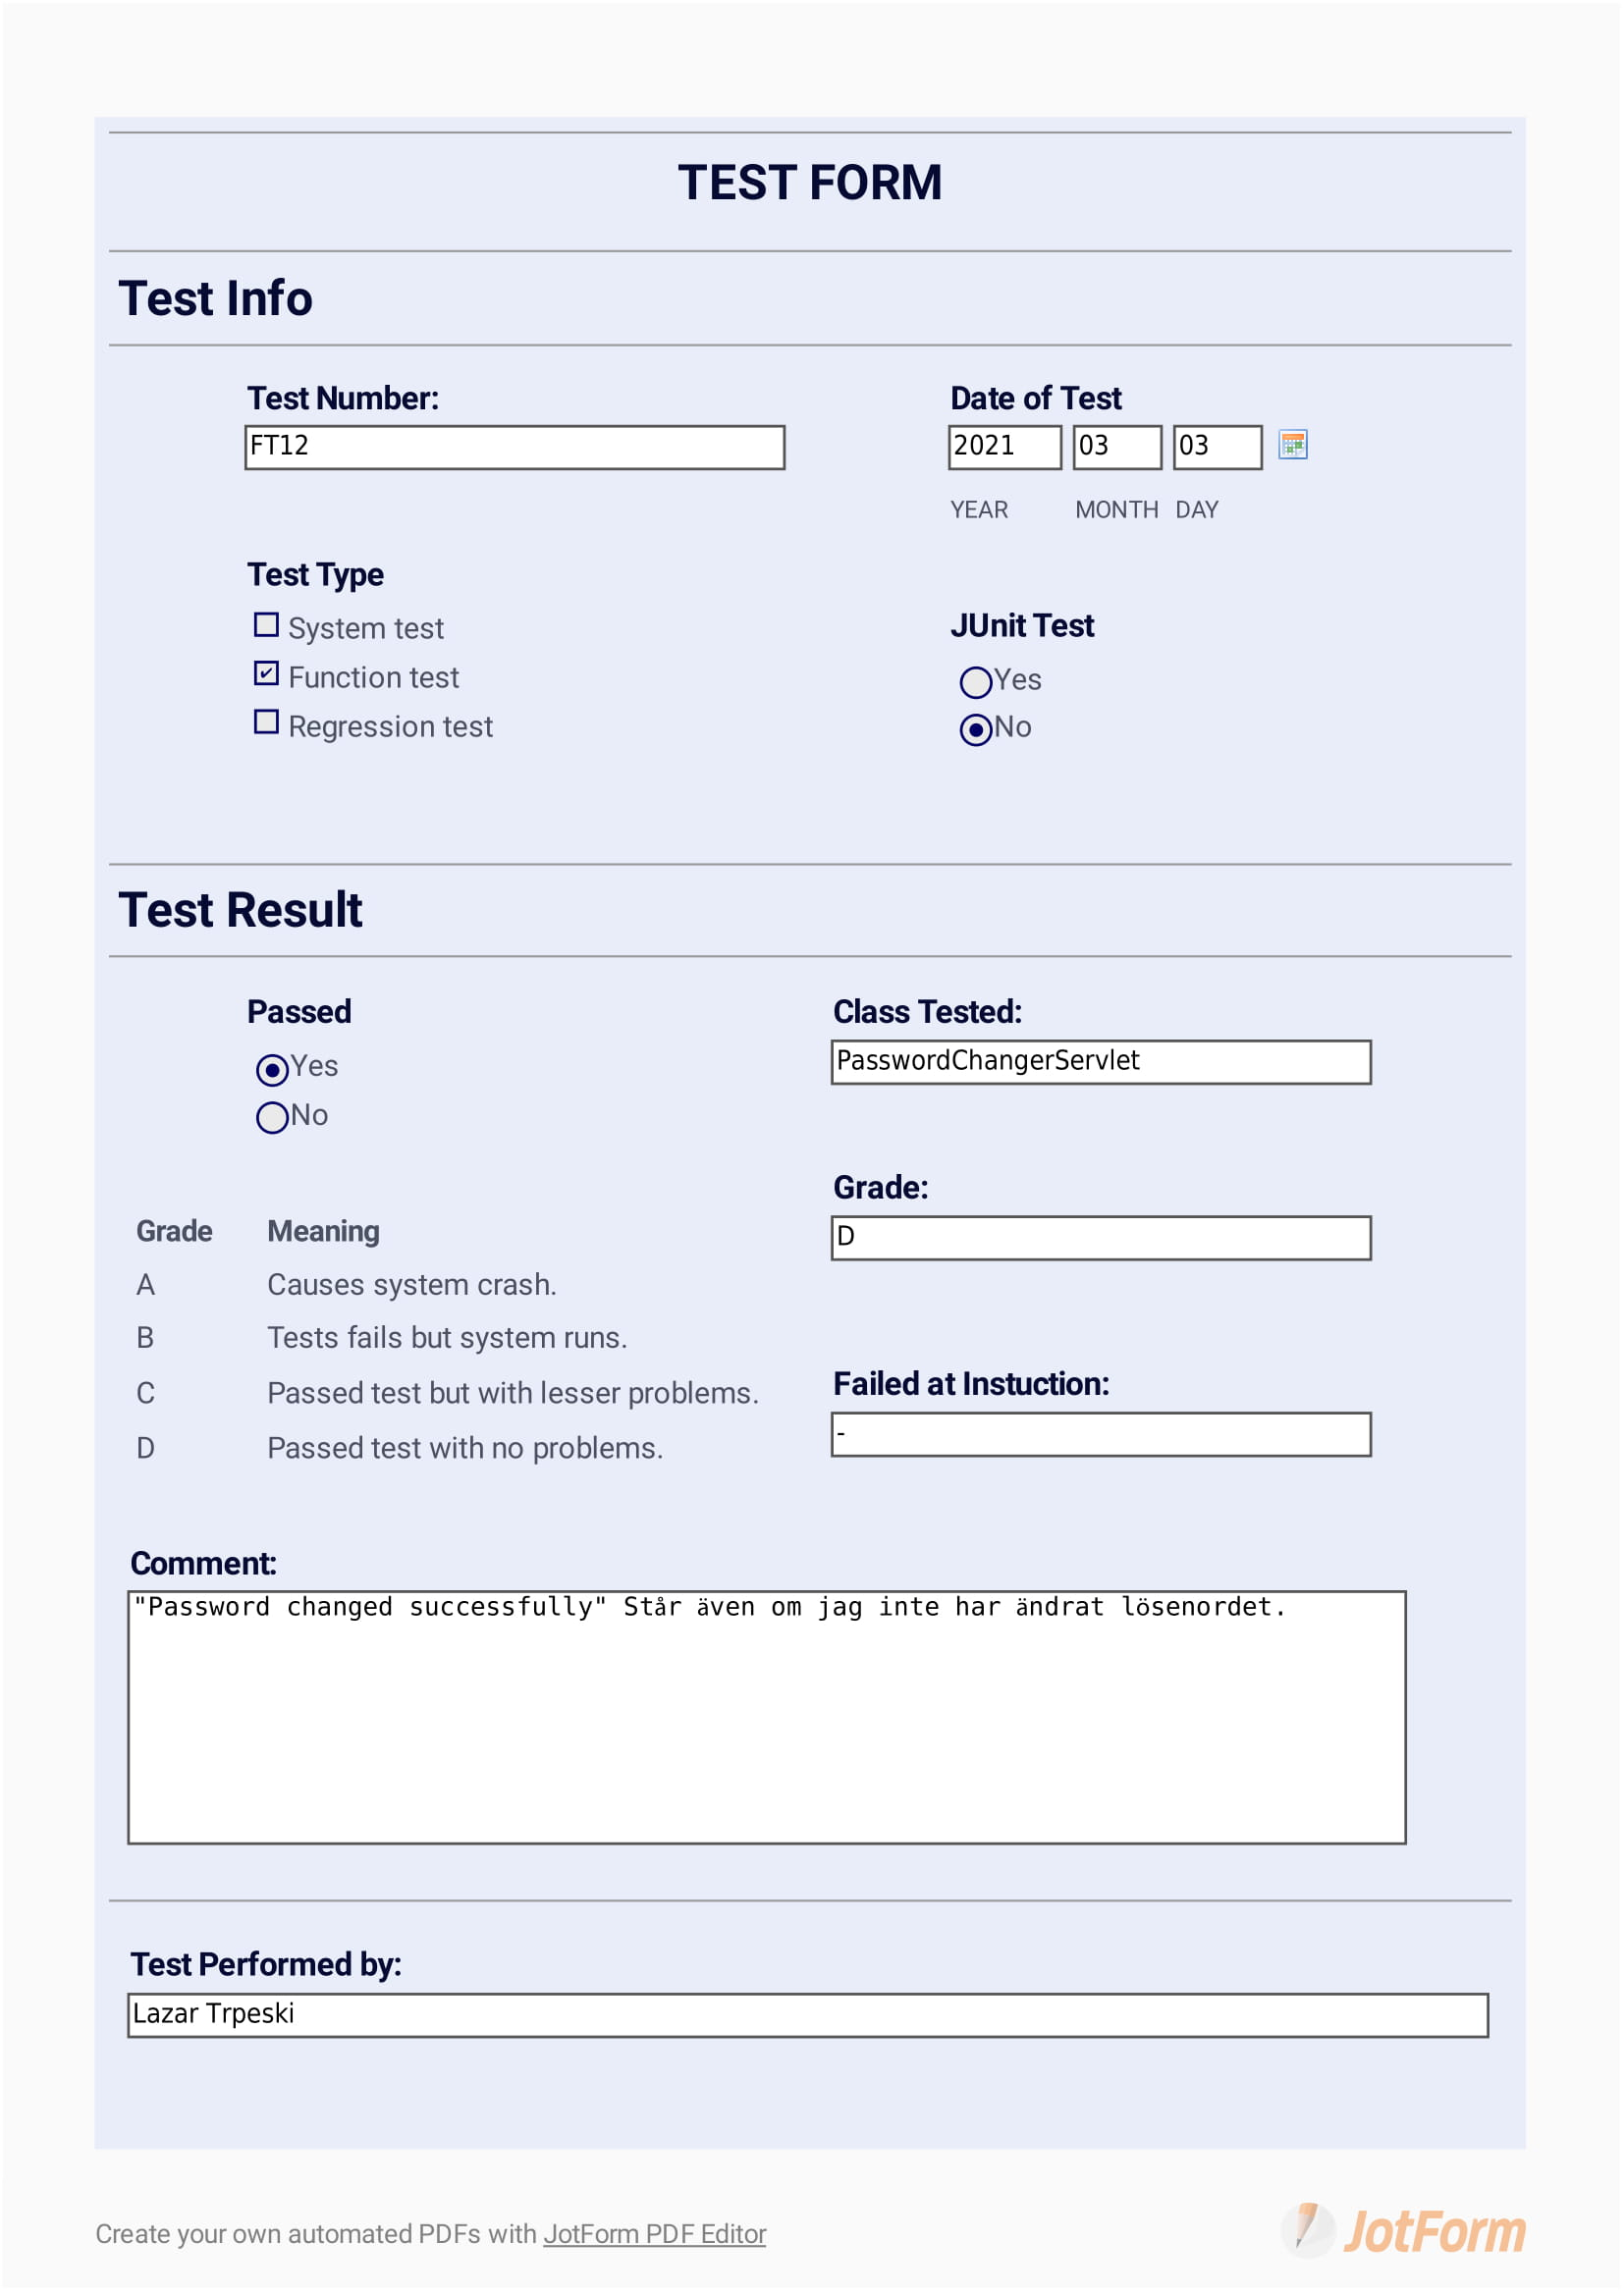
\includegraphics[width=13cm]{images/2021-03-03_Lazar_FT12-1}
     \renewcommand\figurename{Figure}
     \caption{Test form for FT12}
     \label{fig:my_label}
 \end{figure}
 
 \begin{figure}
     \centering
     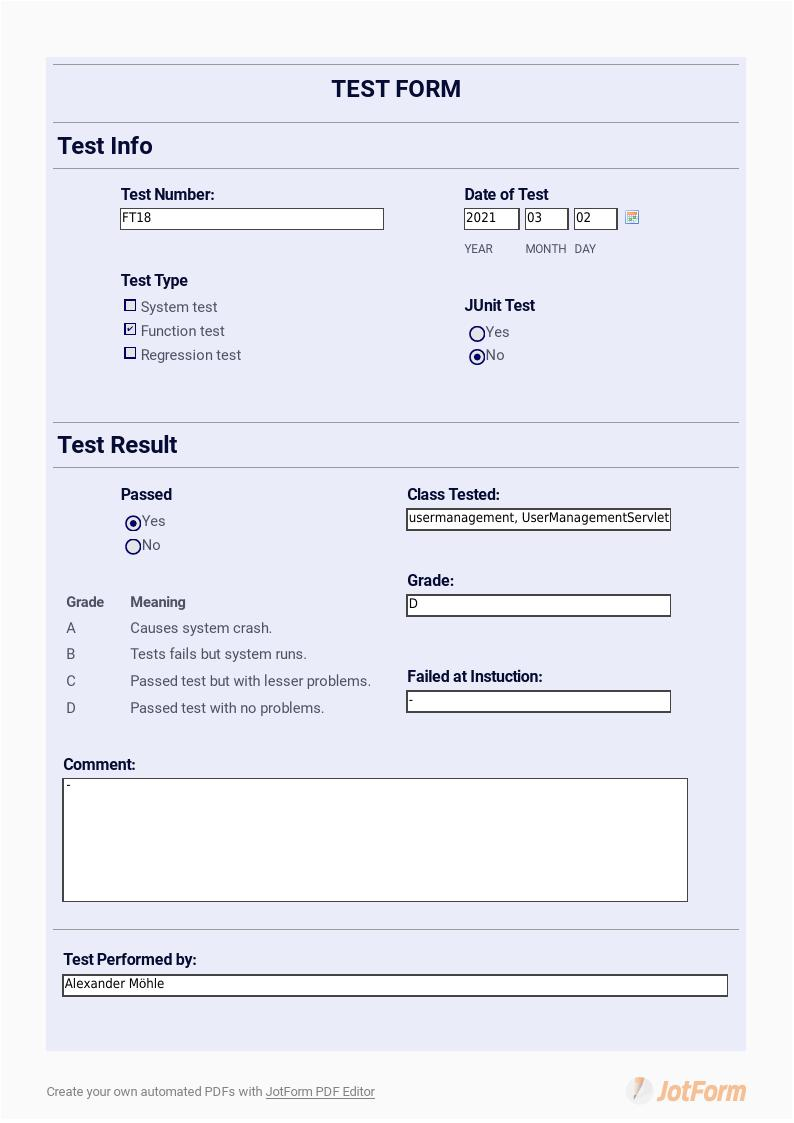
\includegraphics[width=13cm]{images/2021-03-02_Alexander_FT18_001}
     \renewcommand\figurename{Figure}
     \caption{Test form for FT18}
     \label{fig:my_label}
 \end{figure}
 
 \begin{figure}
     \centering
     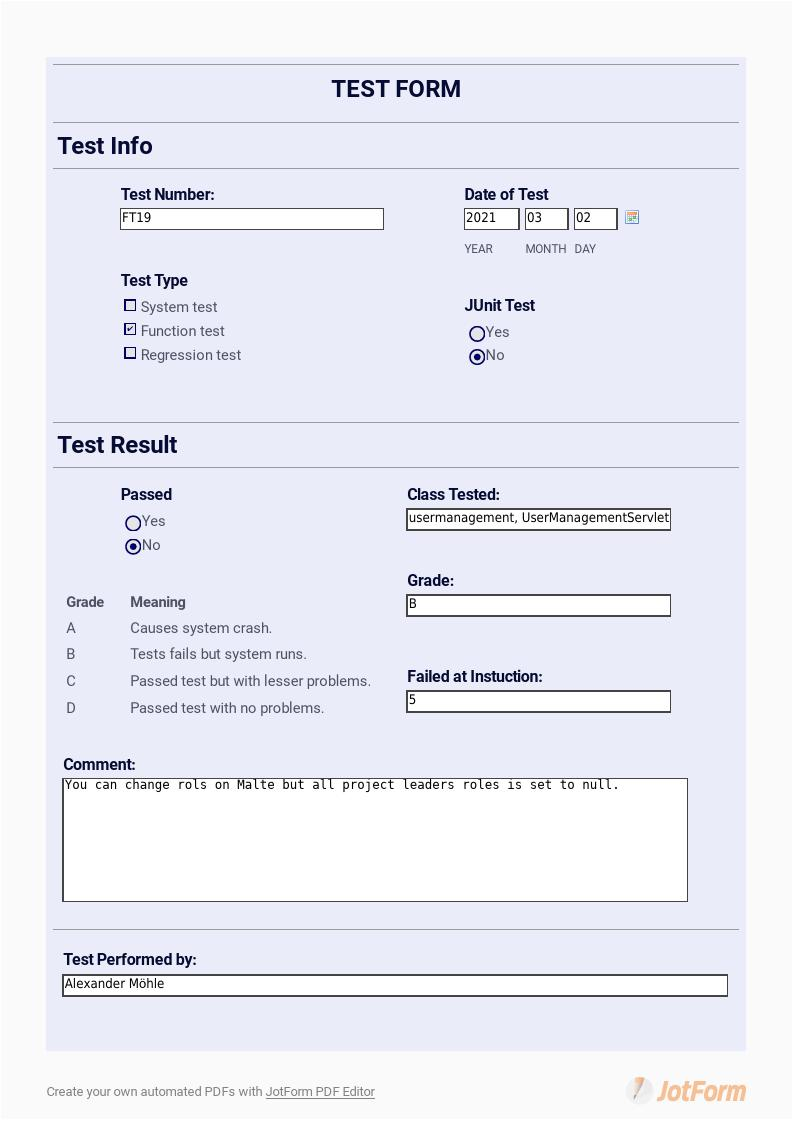
\includegraphics[width=13cm]{images/2021-03-02_Alexander_FT19_001}
     \renewcommand\figurename{Figure}
     \caption{Test form for FT19}
     \label{fig:my_label}
 \end{figure}
 
 \begin{figure}
     \centering
     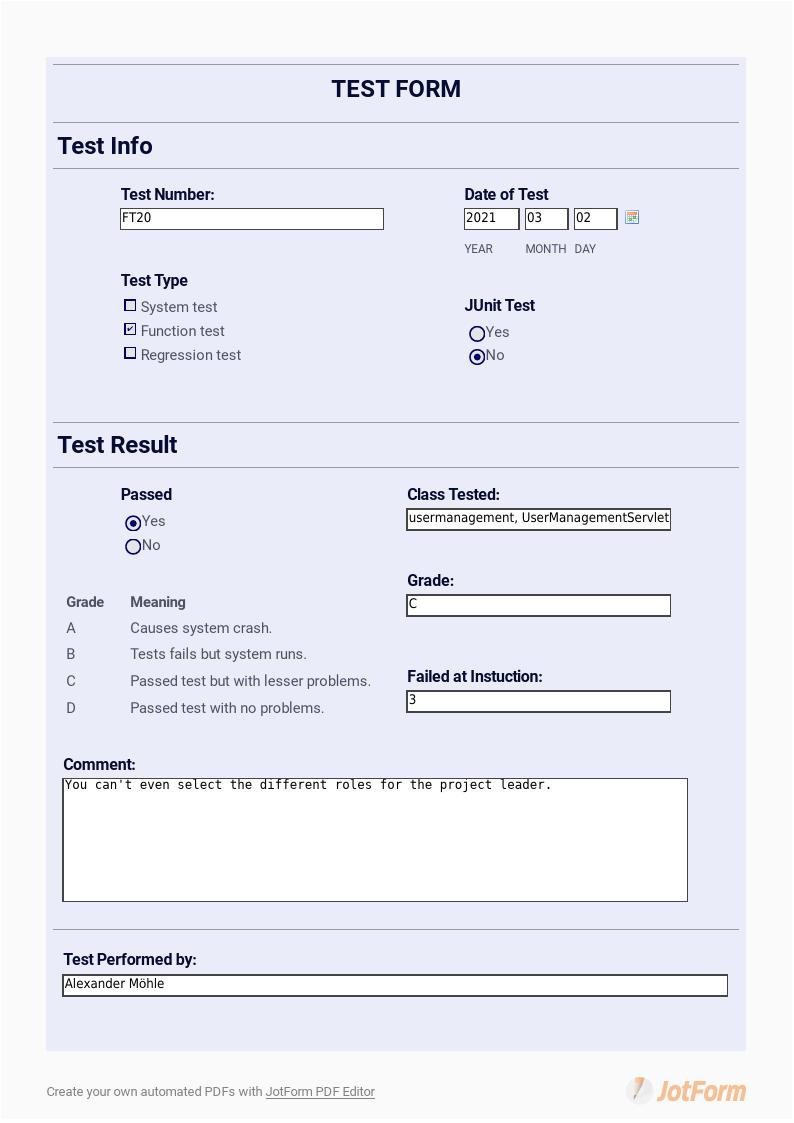
\includegraphics[width=13cm]{images/2021-03-02_Alexander_FT20_001}
     \renewcommand\figurename{Figure}
     \caption{Test form for FT20}
     \label{fig:my_label}
 \end{figure}
 
 \begin{figure}
     \centering
     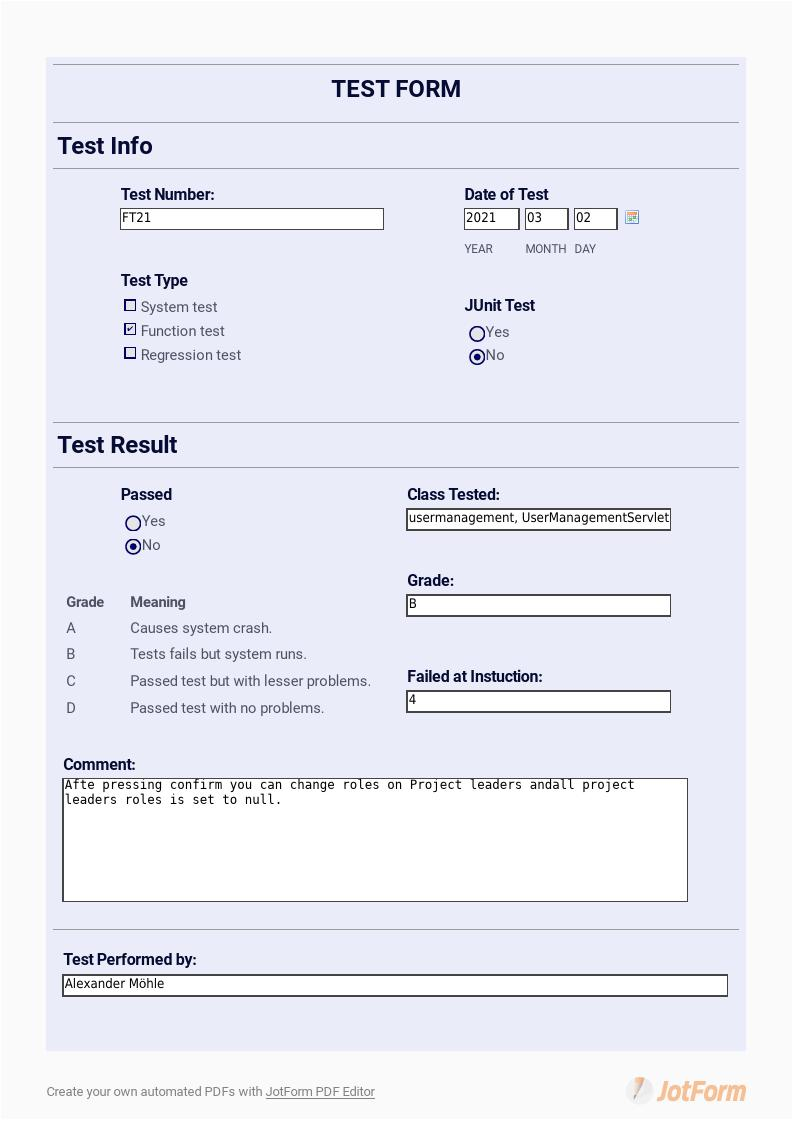
\includegraphics[width=13cm]{images/2021-03-02_Alexander_FT21_001}
     \renewcommand\figurename{Figure}
     \caption{Test form for FT21}
     \label{fig:my_label}
 \end{figure}
 
 \begin{figure}
     \centering
     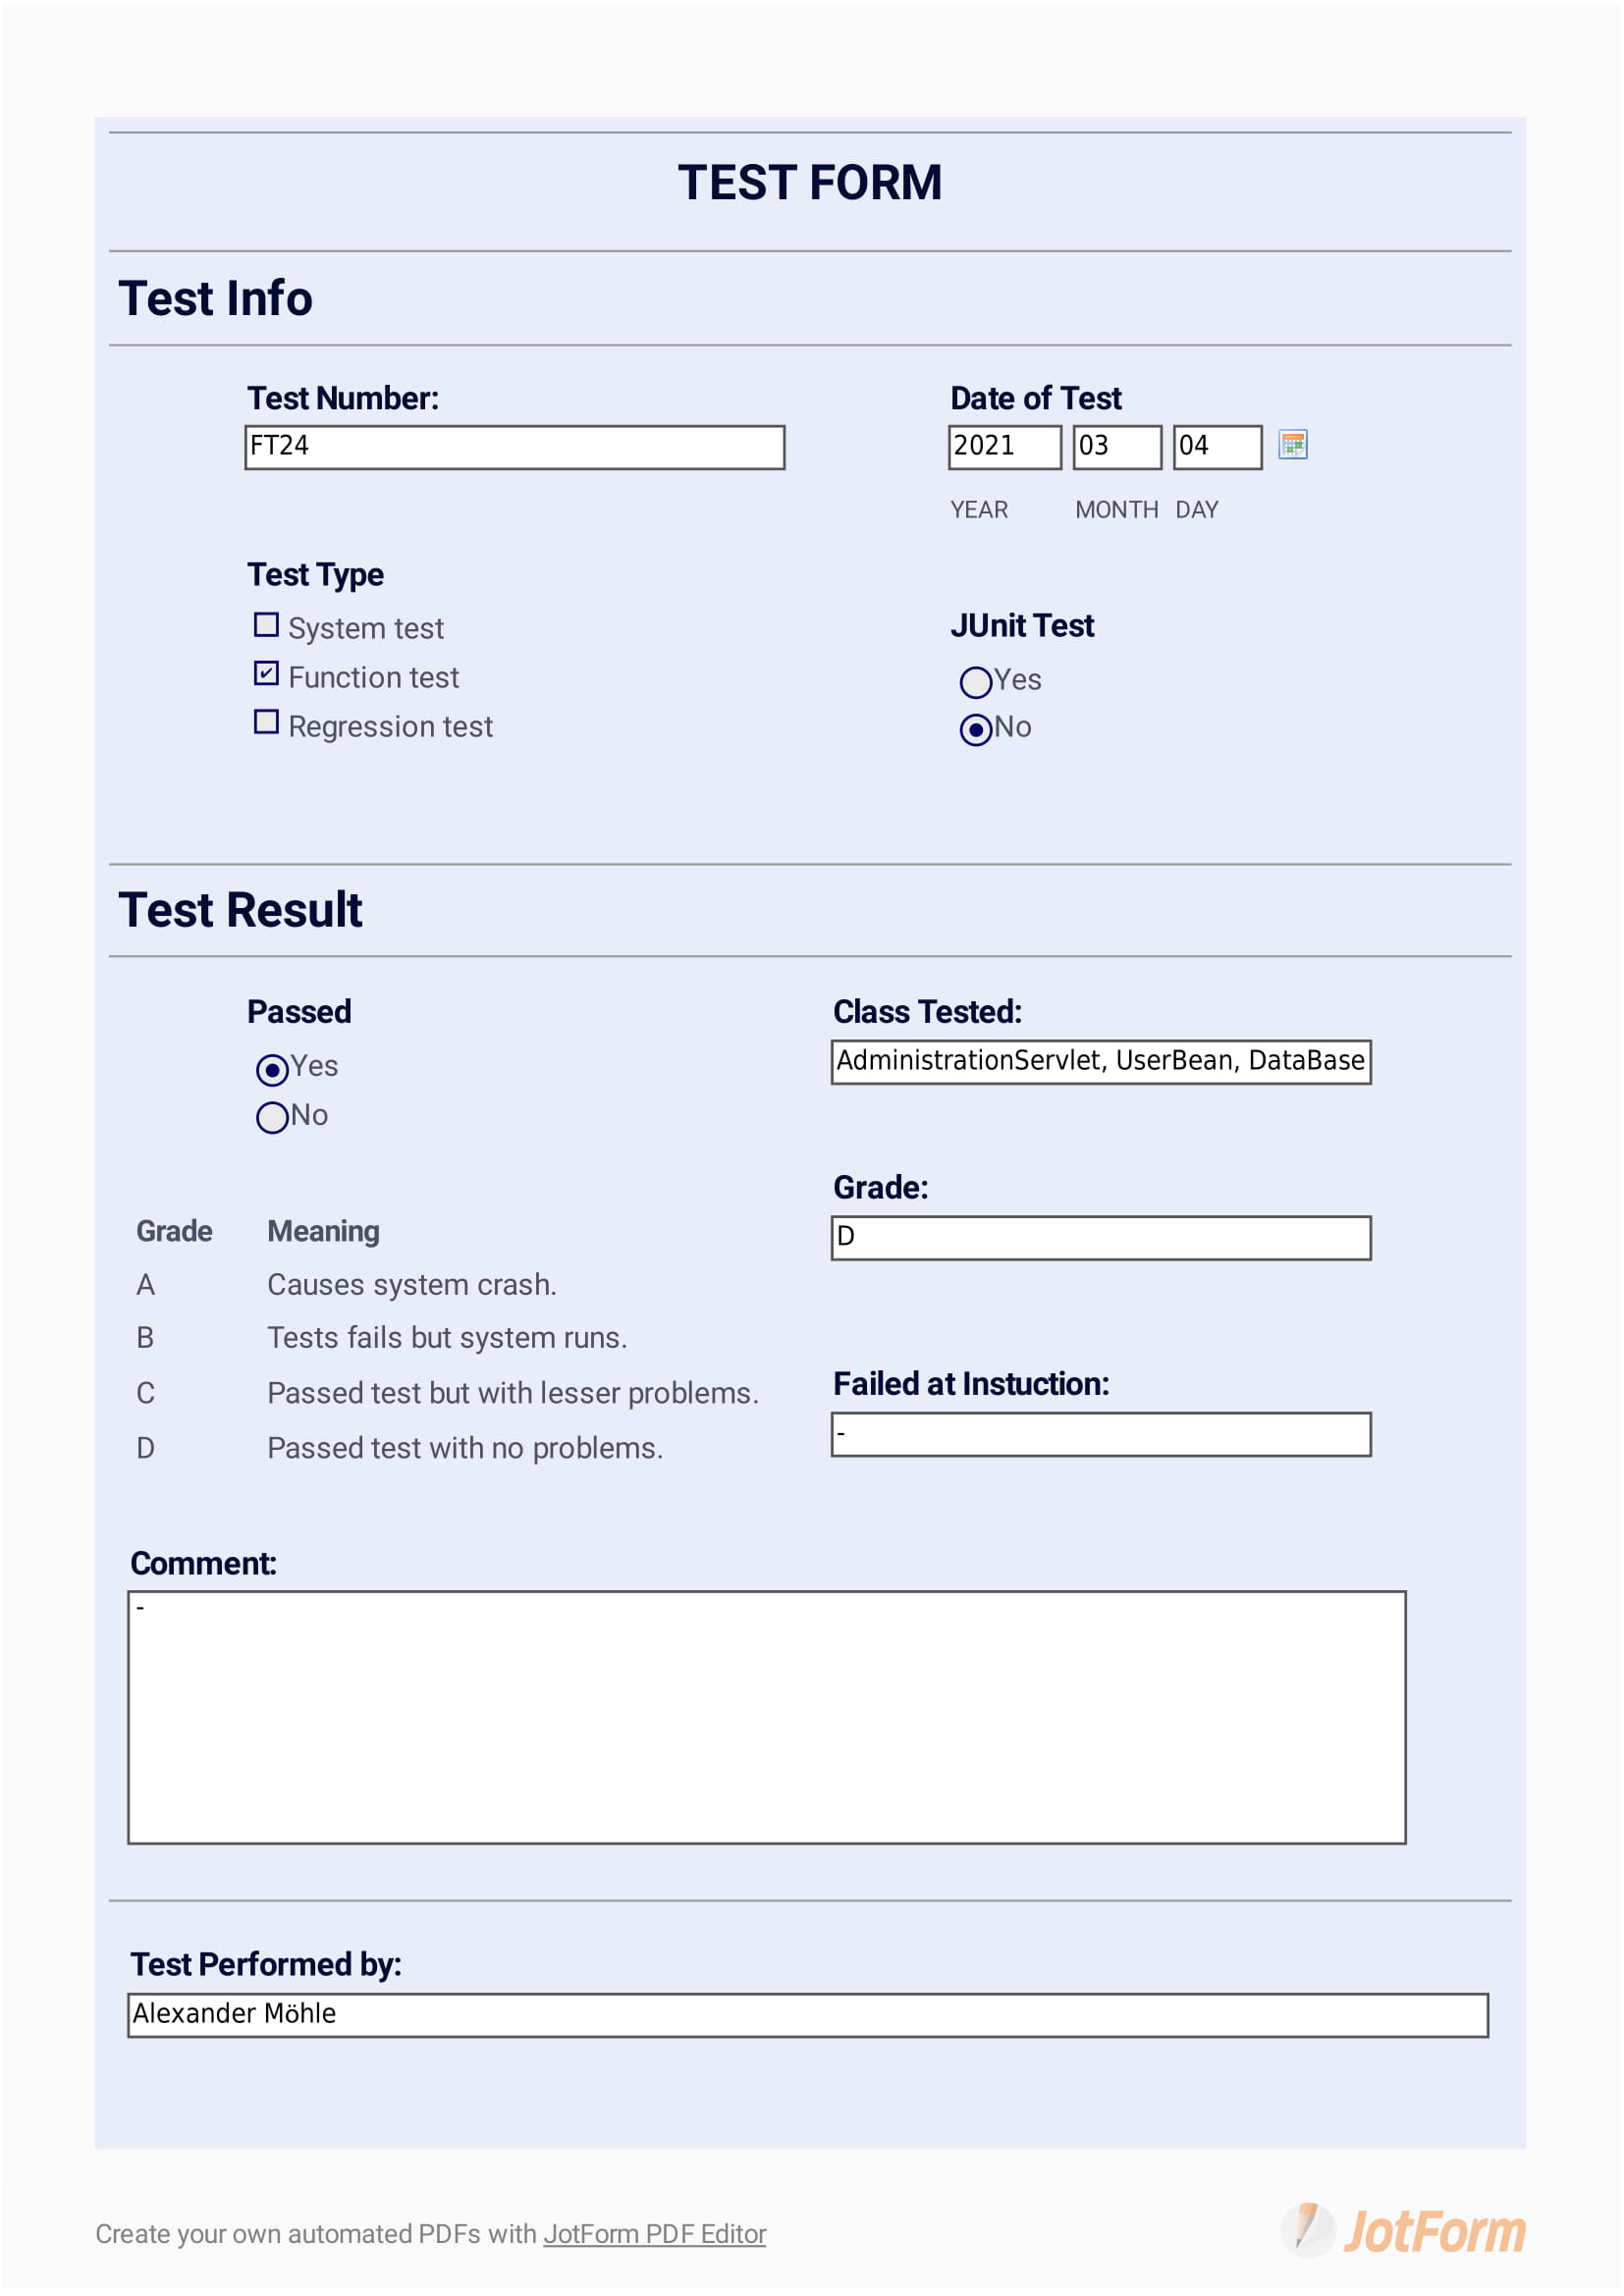
\includegraphics[width=13cm]{images/2021-03-04_Alexander_FT24-1}
     \renewcommand\figurename{Figure}
     \caption{Test form for FT24}
     \label{fig:my_label}
 \end{figure}
 
 \begin{figure}
     \centering
     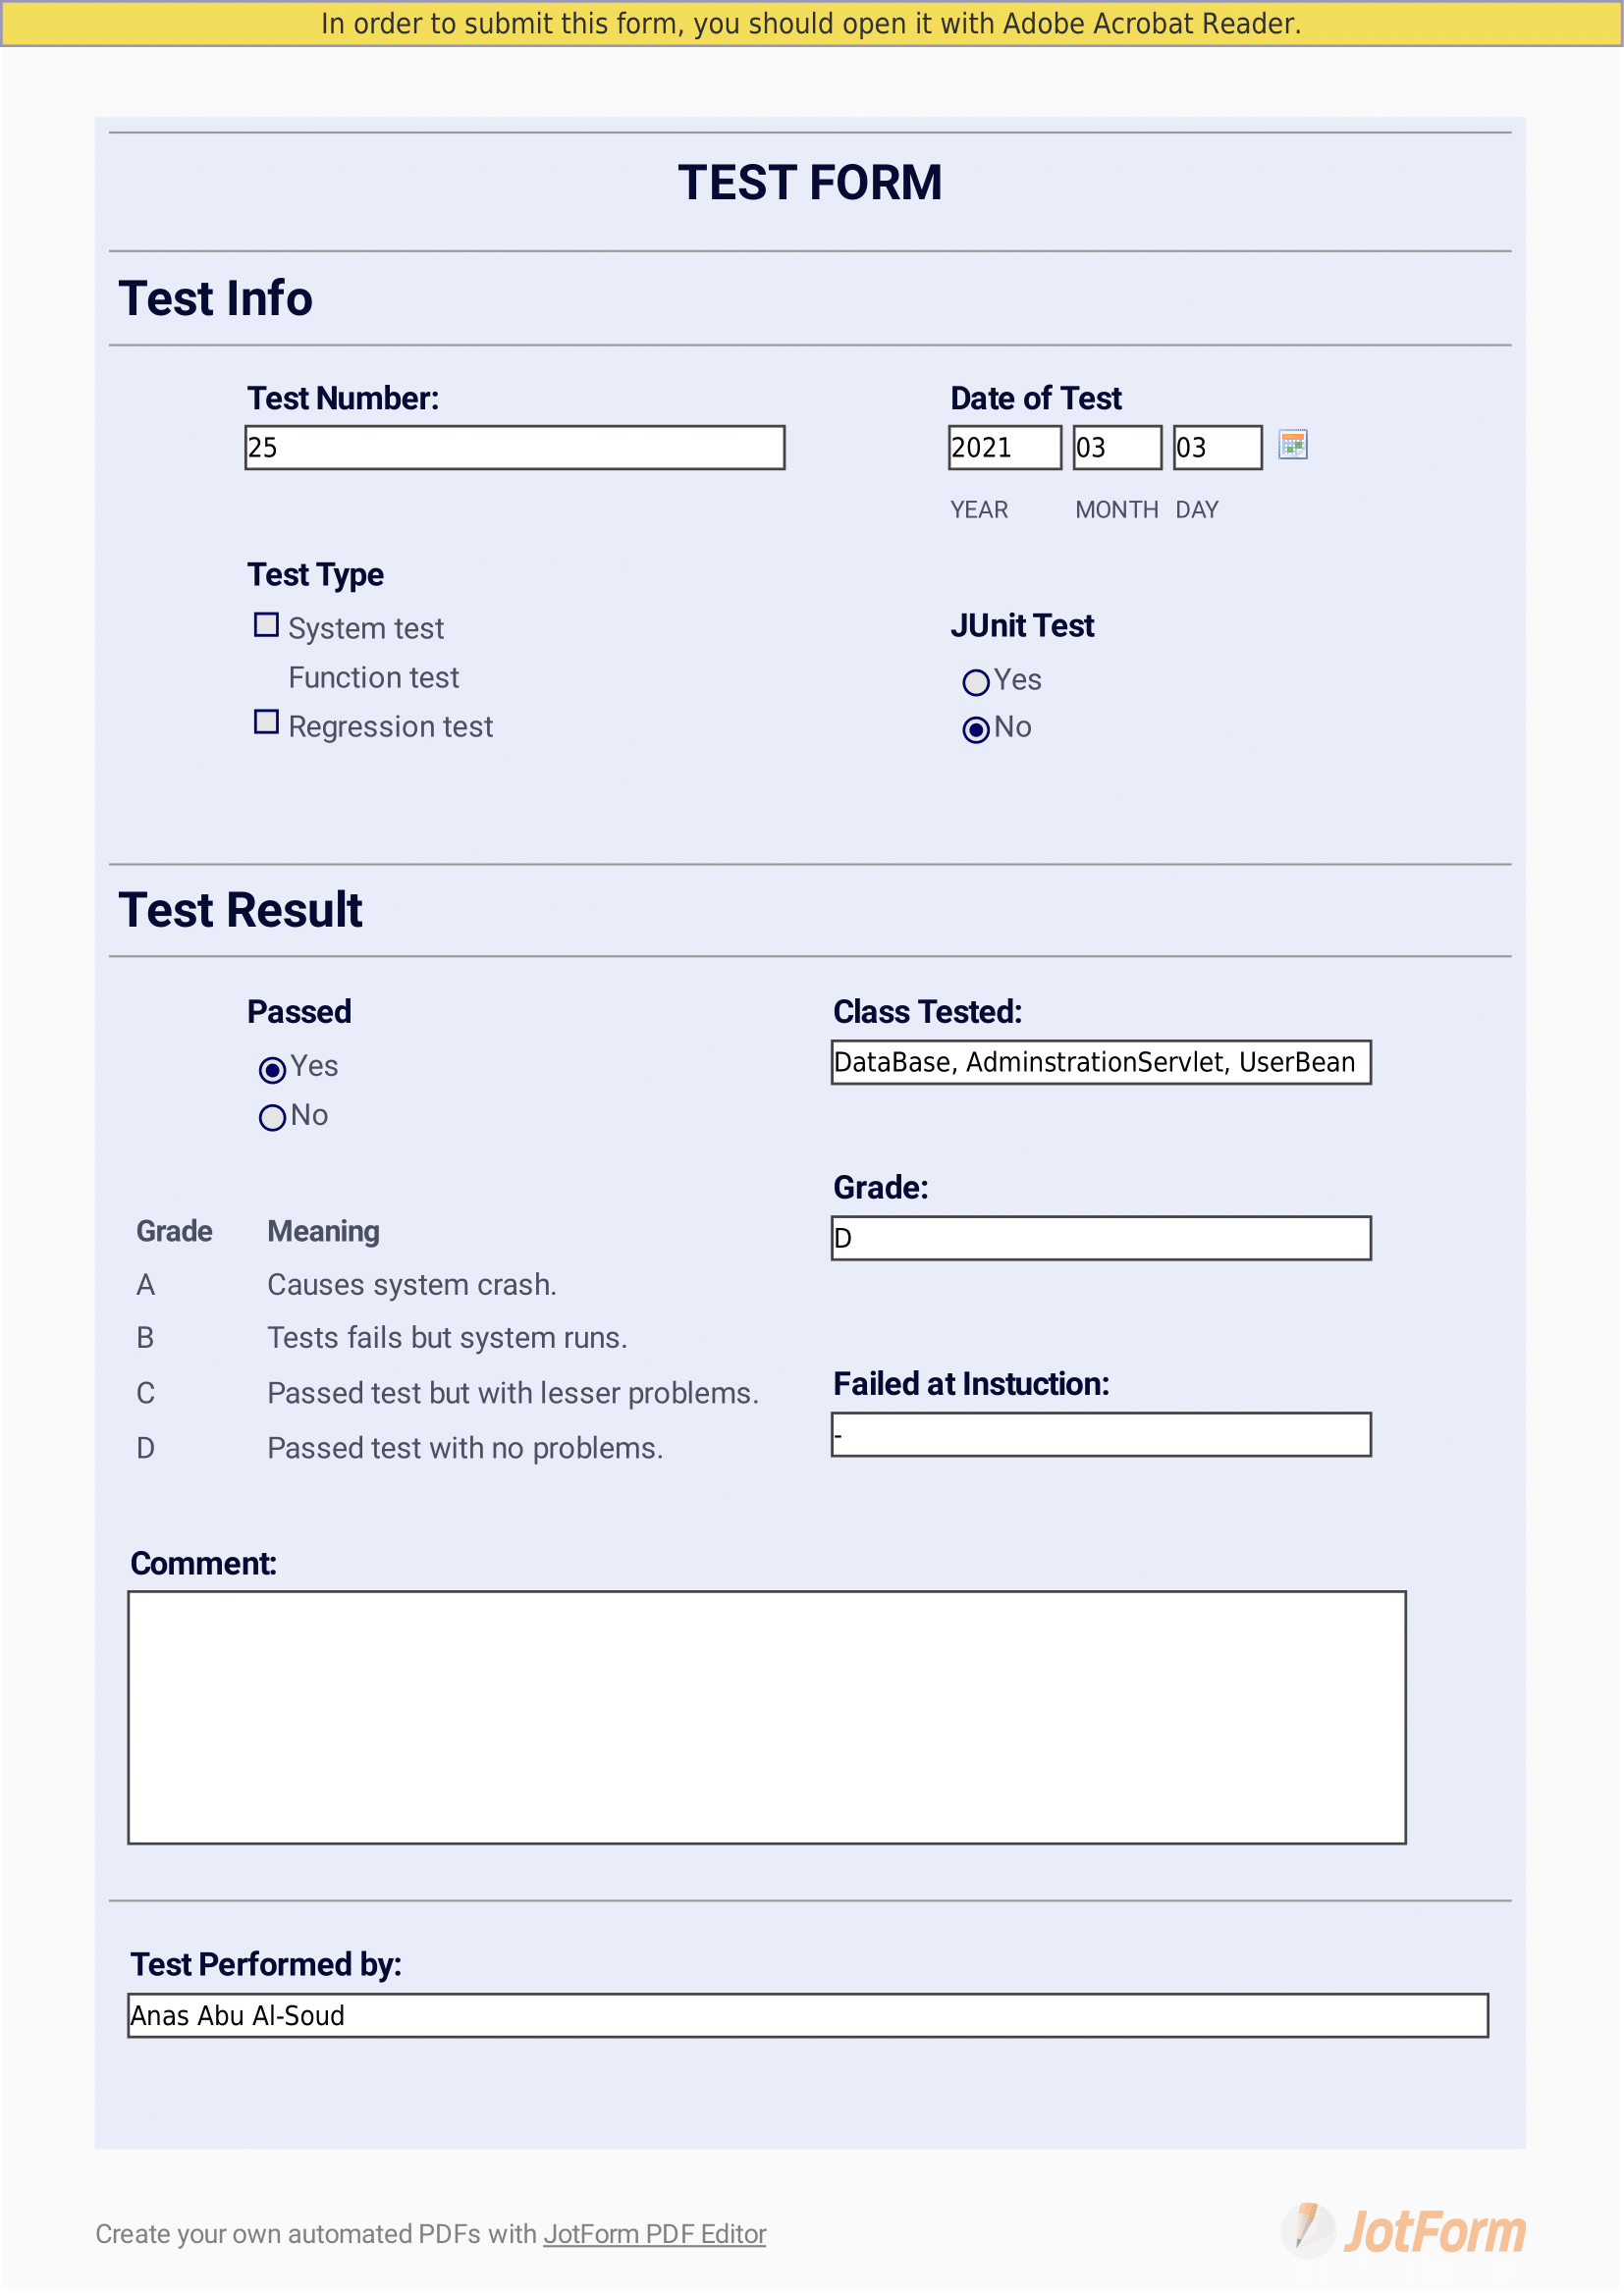
\includegraphics[width=13cm]{images/2021-03-03_Anas_FT25-1}
     \renewcommand\figurename{Figure}
     \caption{Test form for FT25}
     \label{fig:my_label}
 \end{figure}
 
 \begin{figure}
     \centering
     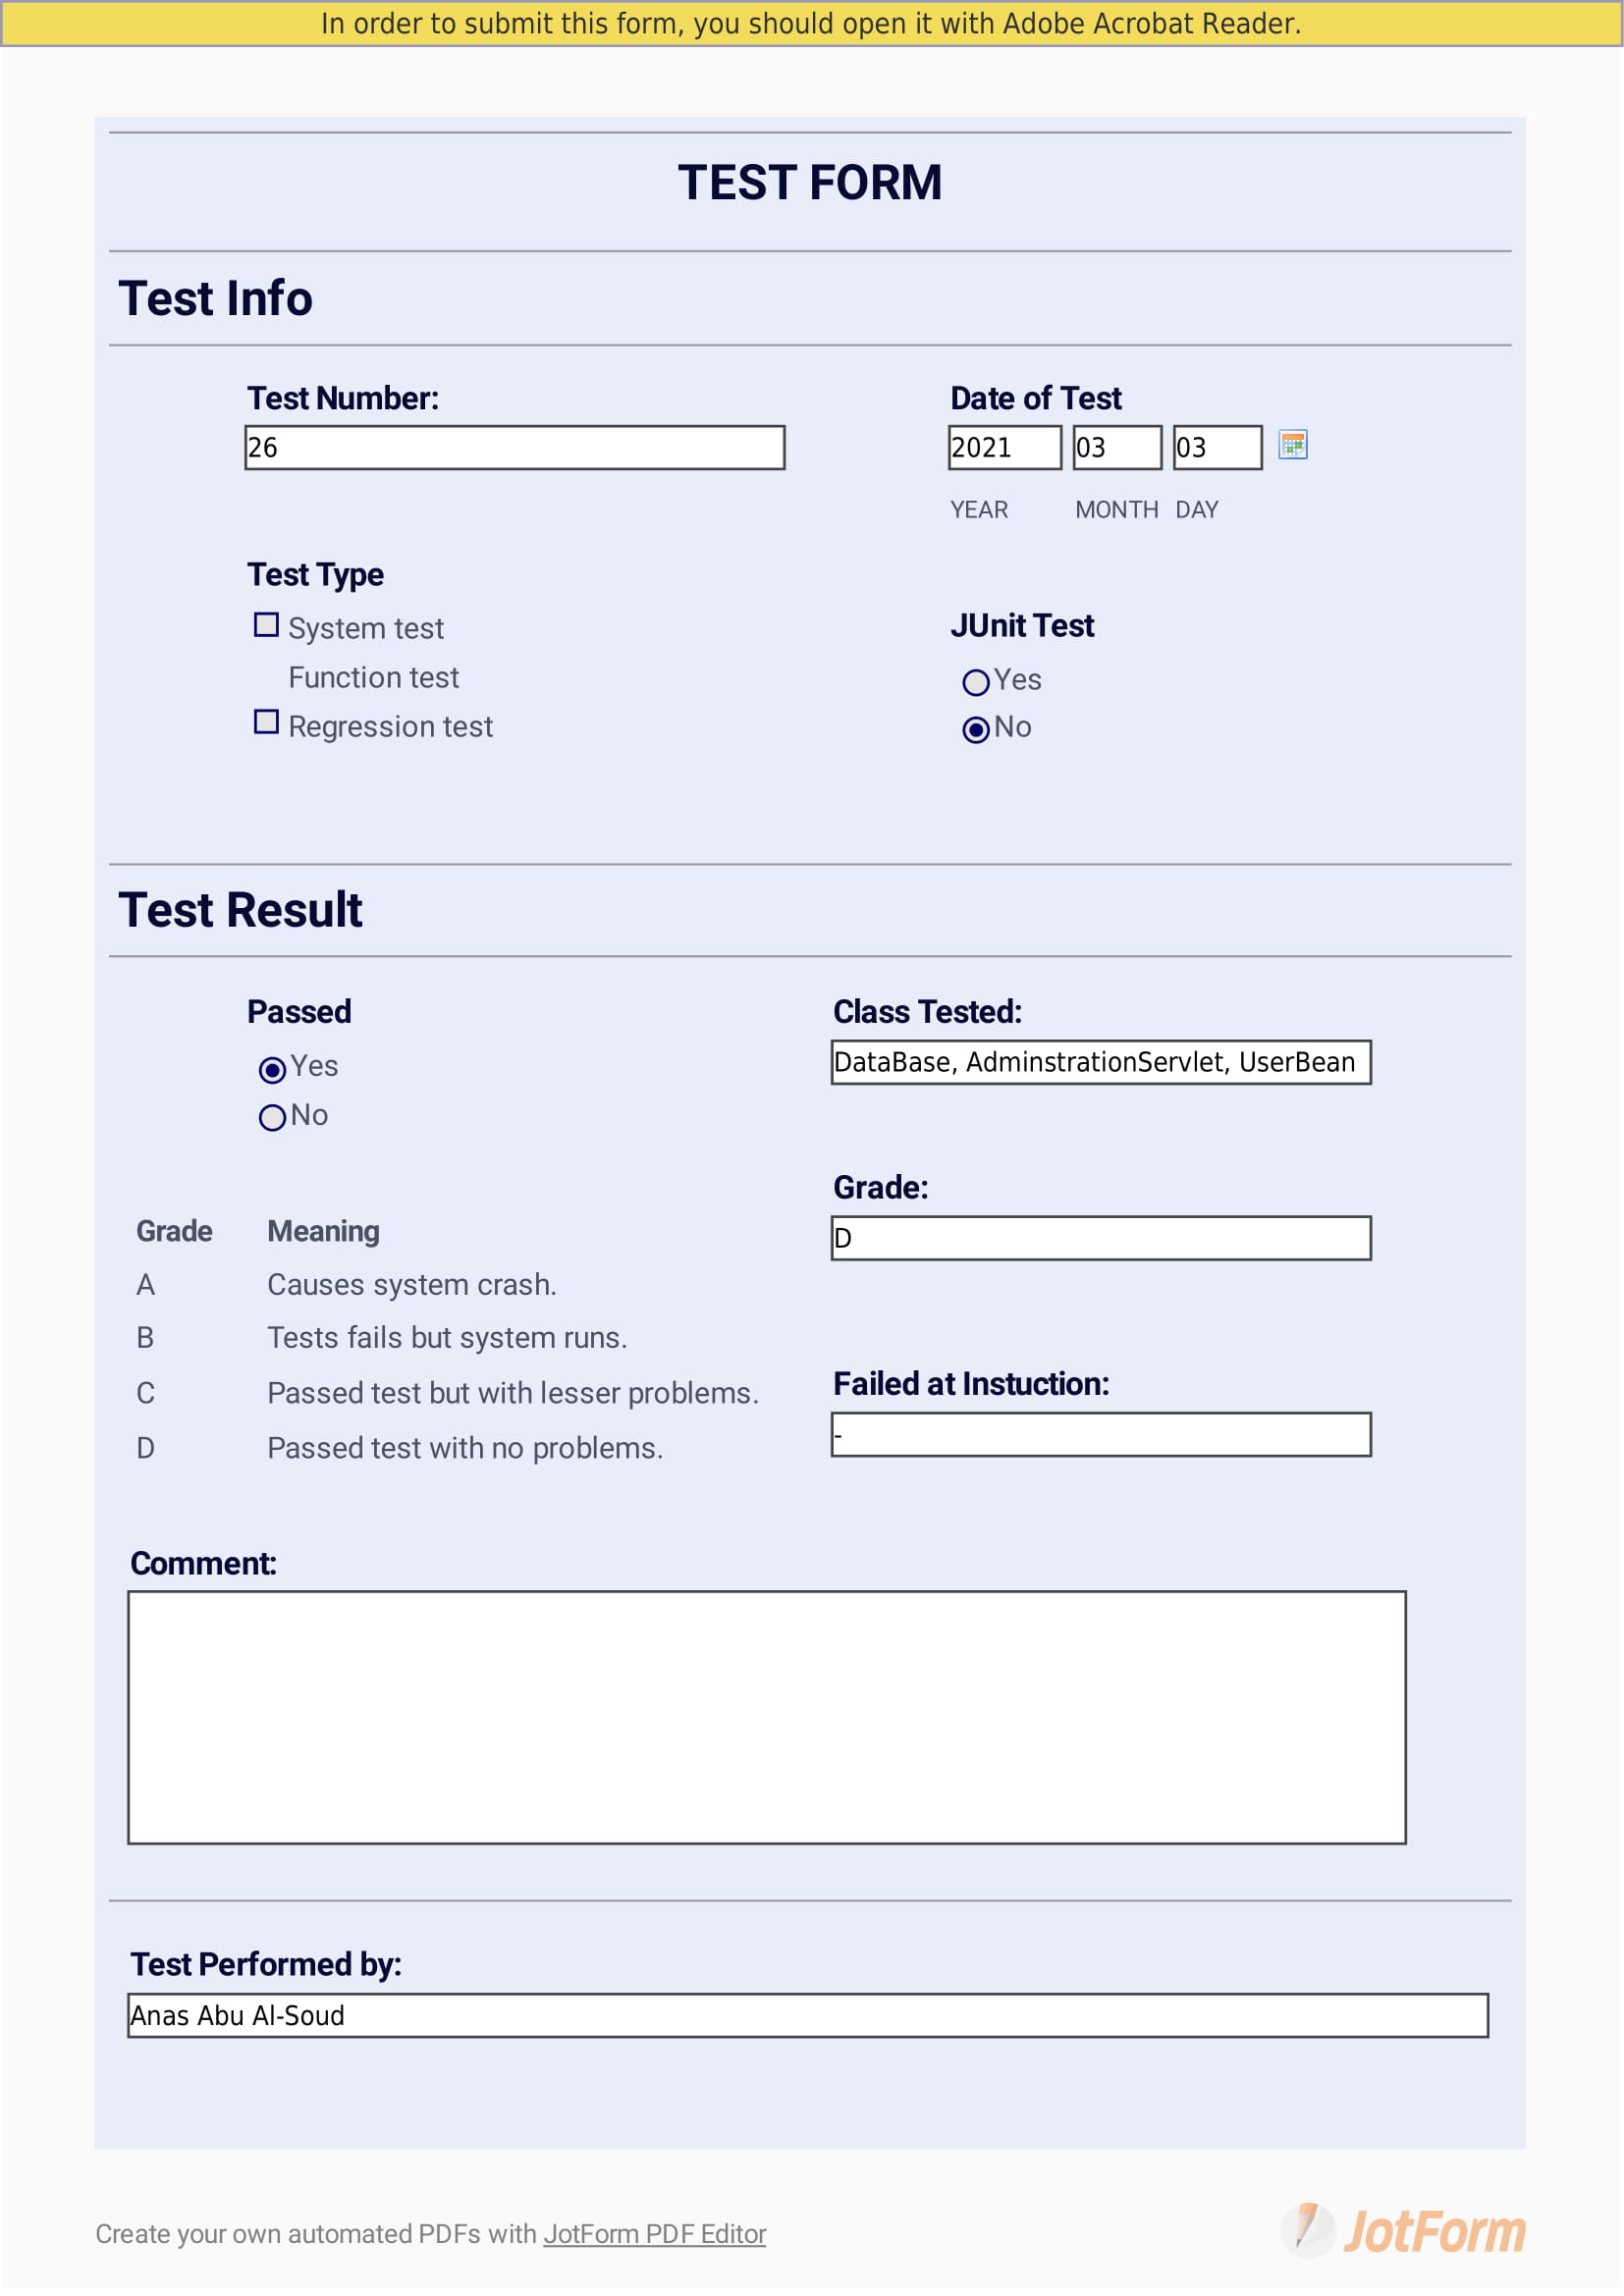
\includegraphics[width=13cm]{images/2021-03-03_Anas_FT26-1}
     \renewcommand\figurename{Figure}
     \caption{Test form for FT26}
     \label{fig:my_label}
 \end{figure}
 
 \begin{figure}
     \centering
     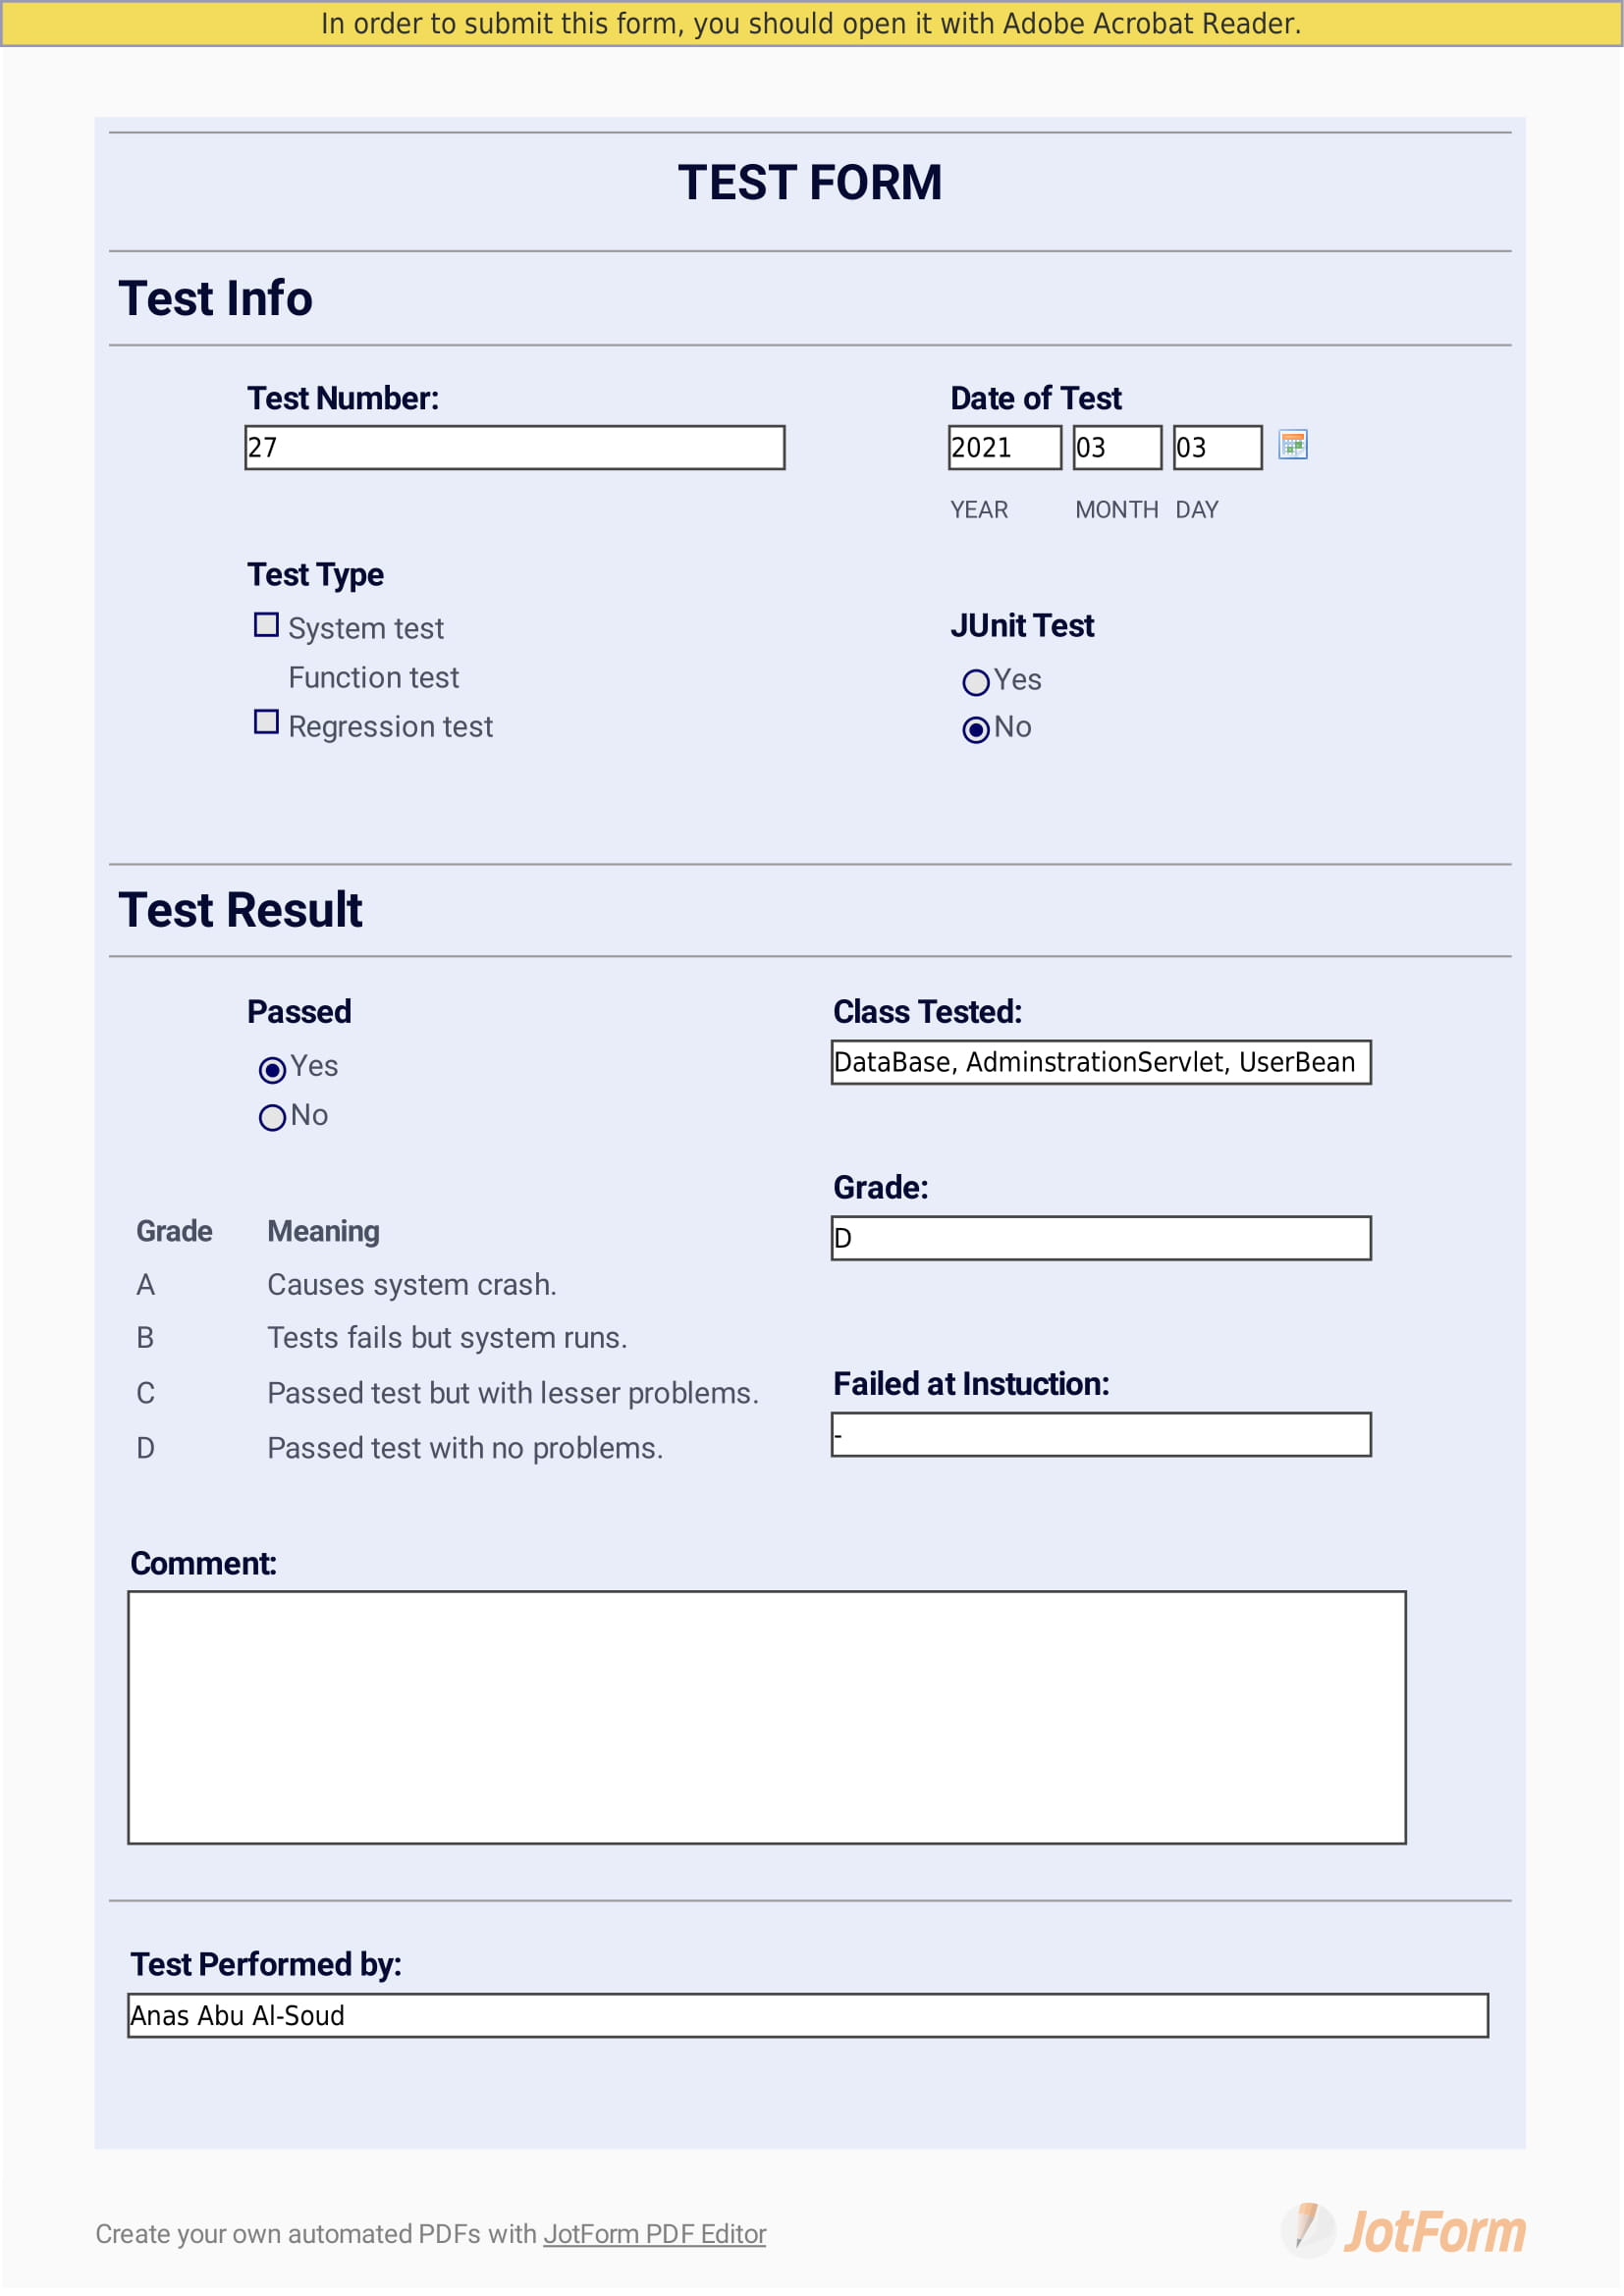
\includegraphics[width=13cm]{images/2021-03-03_Anas_FT27-1}
     \renewcommand\figurename{Figure}
     \caption{Test form for FT27}
     \label{fig:my_label}
 \end{figure}
 
 \begin{figure}
     \centering
     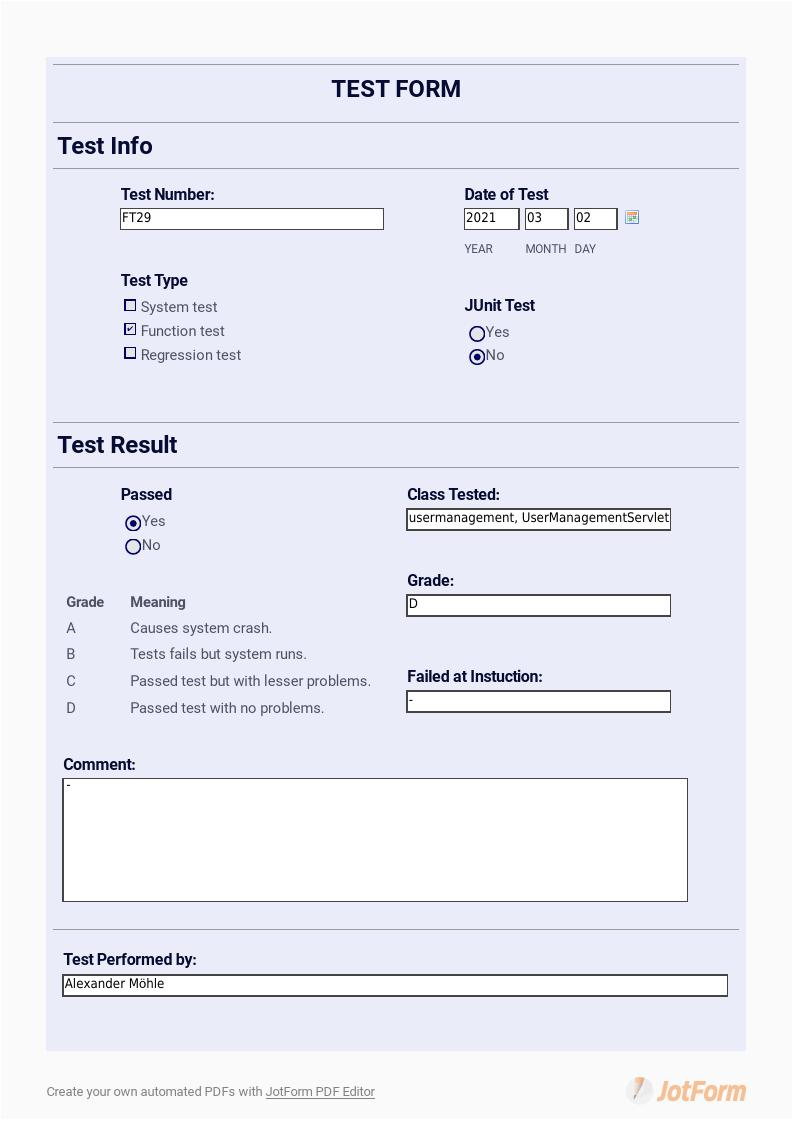
\includegraphics[width=13cm]{images/2021-03-02_Alexander_FT29_001}
     \renewcommand\figurename{Figure}
     \caption{Test form for FT29}
     \label{fig:my_label}
 \end{figure}
 
 \begin{figure}
     \centering
     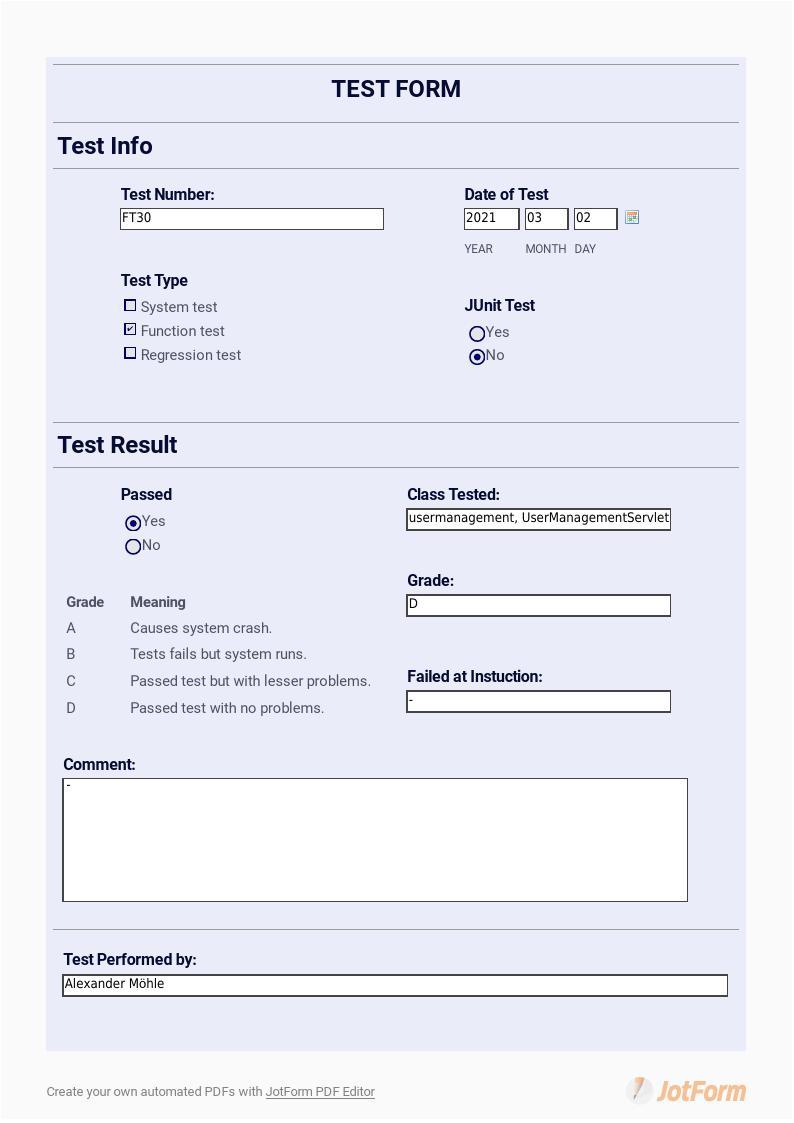
\includegraphics[width=13cm]{images/2021-03-02_Alexander_FT30_001}
     \renewcommand\figurename{Figure}
     \caption{Test form for FT30}
     \label{fig:my_label}
 \end{figure}
 
 \begin{figure}
     \centering
     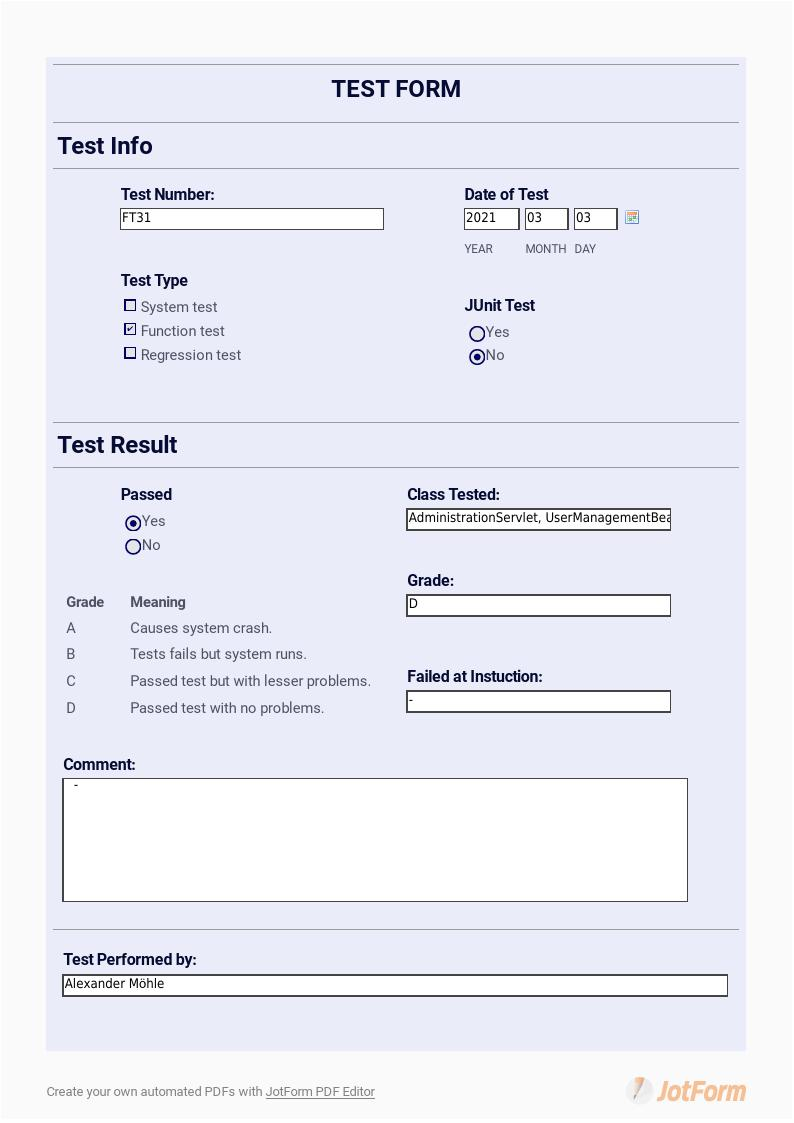
\includegraphics[width=13cm]{images/2021-03-03_Alexander_FT31_001}
     \renewcommand\figurename{Figure}
     \caption{Test form for FT31}
     \label{fig:my_label}
 \end{figure}


\newpage
\begin{flushleft}
{\large \textbf{B. System Test Result}}
\end{flushleft}

\vspace*{\fill}
                \hfill
                \begin{center}
                This page unintentionally left blank.
                \end{center}
                \vspace{\fill}
                \thispagestyle{empty}

\begin{figure}
     \centering
     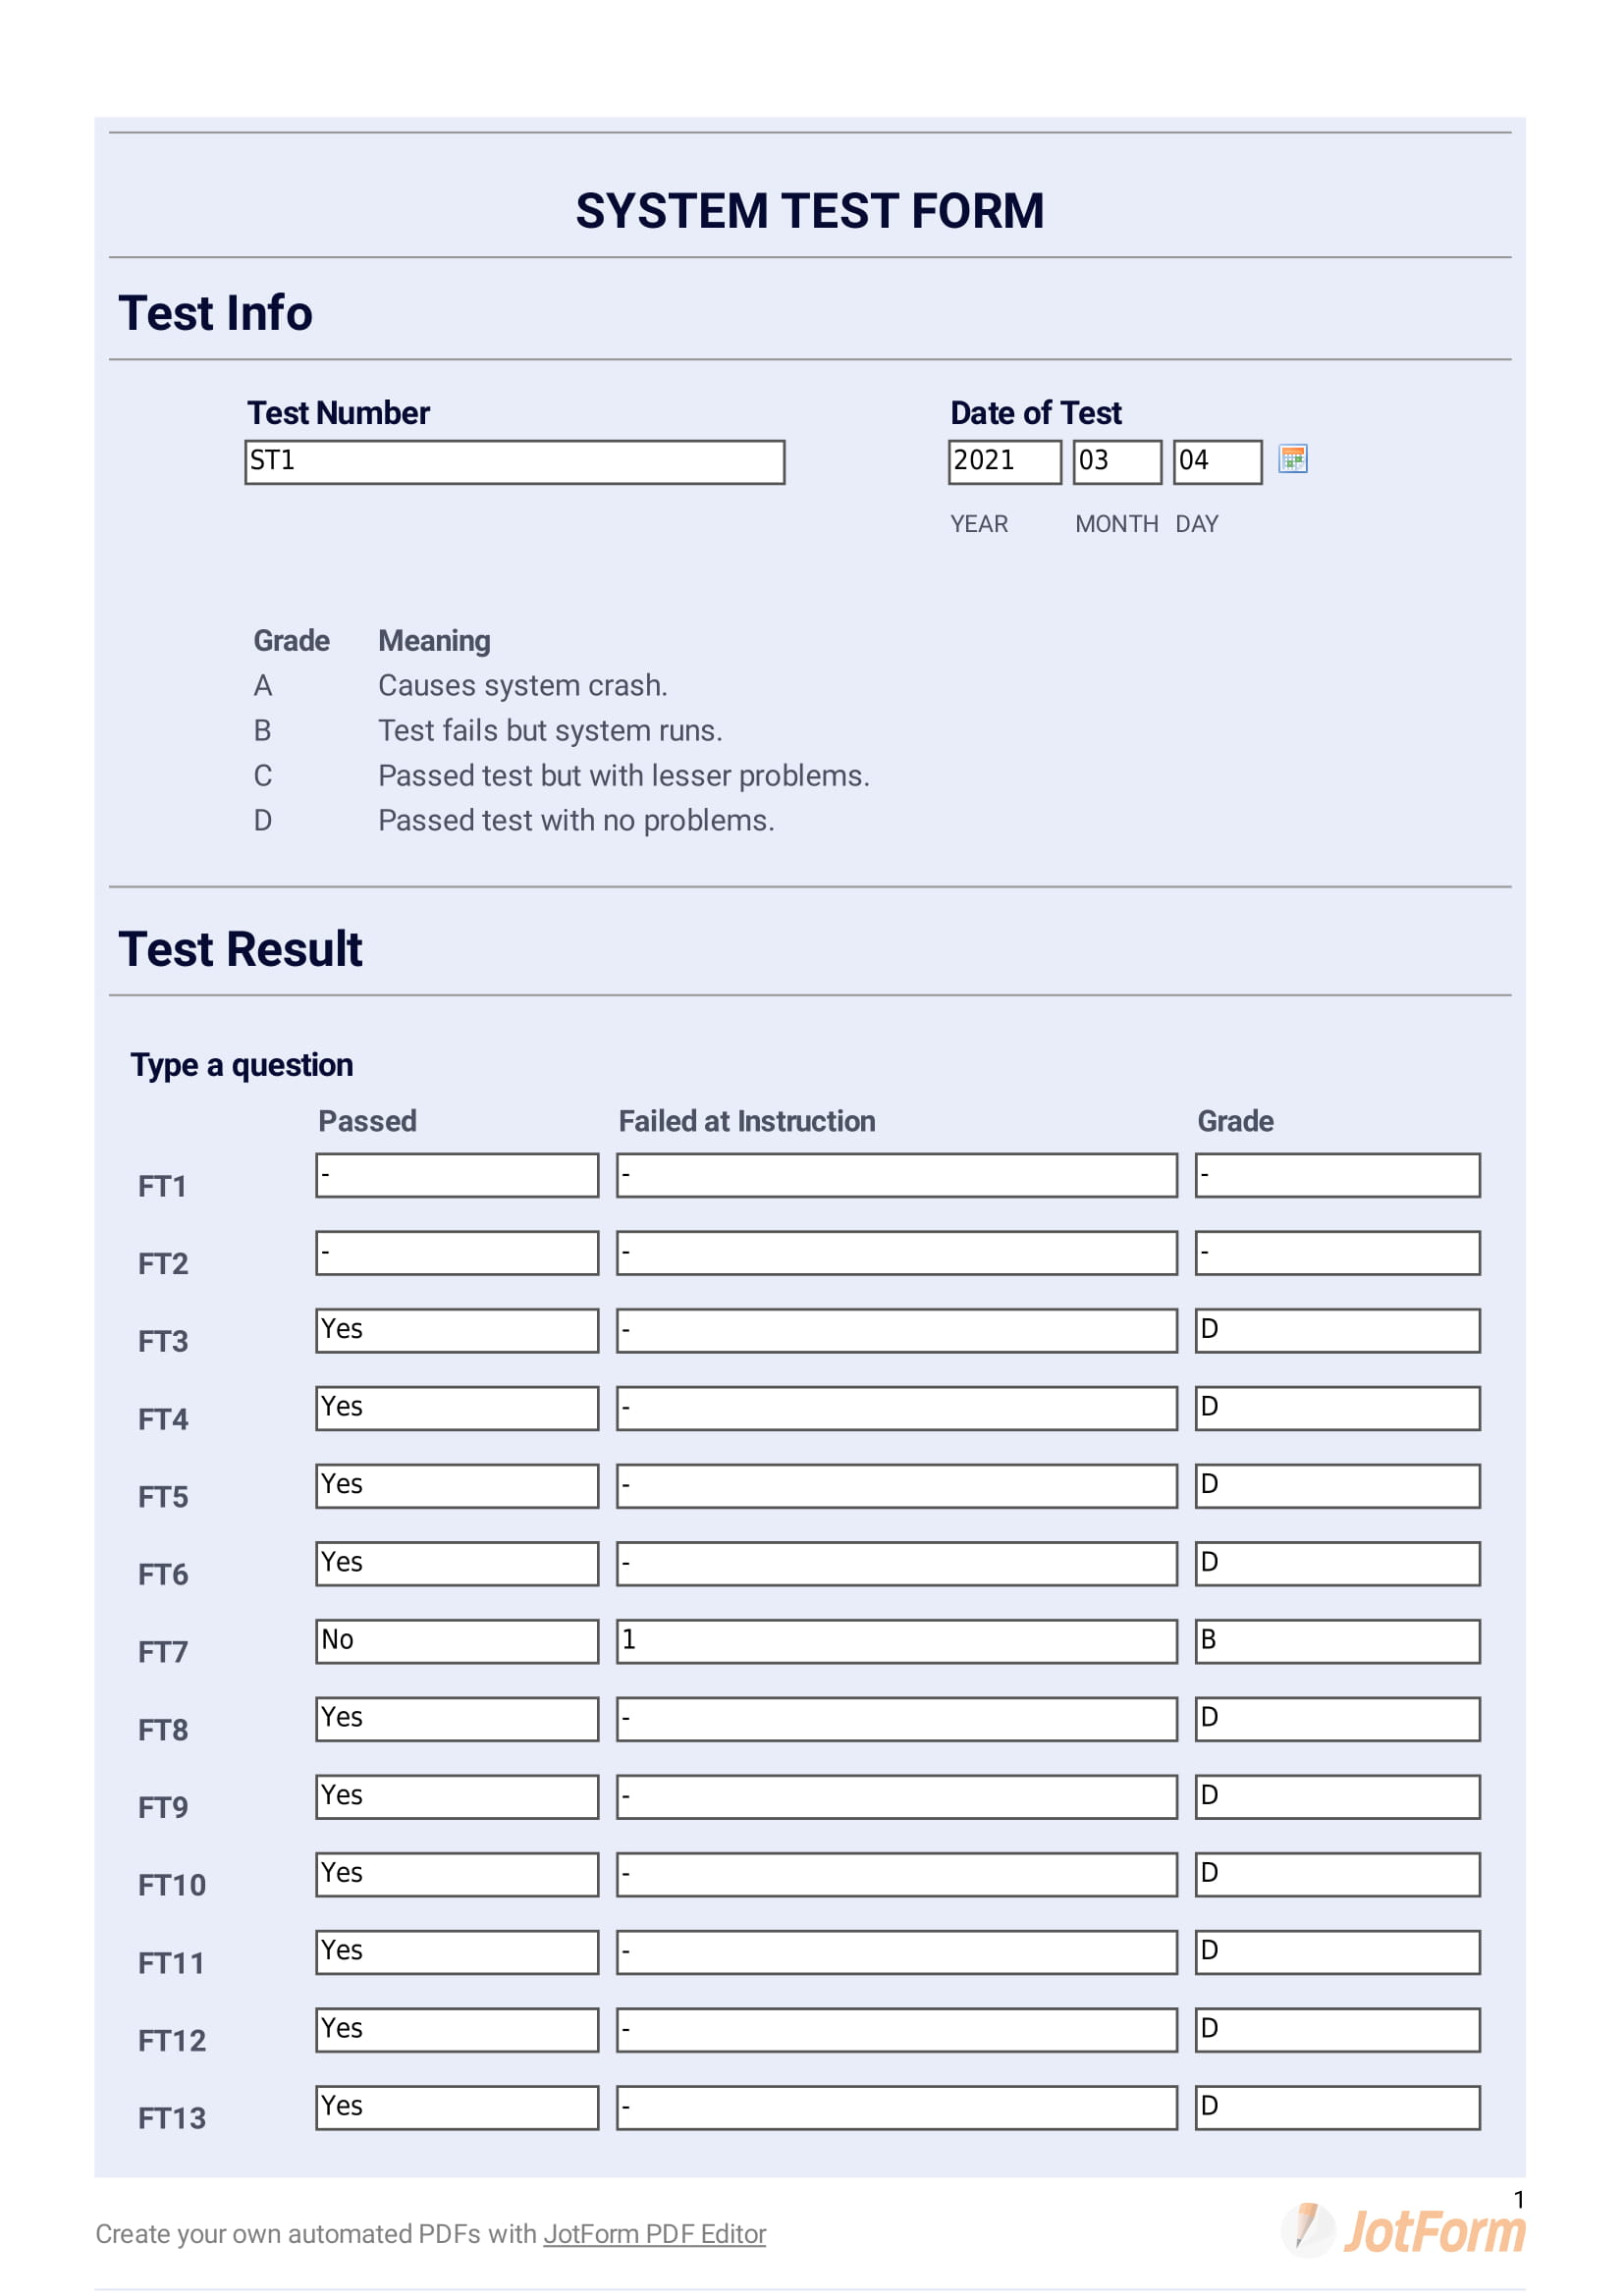
\includegraphics[width=13cm]{images/2021-03-04_Alexander_ST1-1}
     \renewcommand\figurename{Figure}
     \label{fig:my_label}
 \end{figure}
 
 \begin{figure}
     \centering
     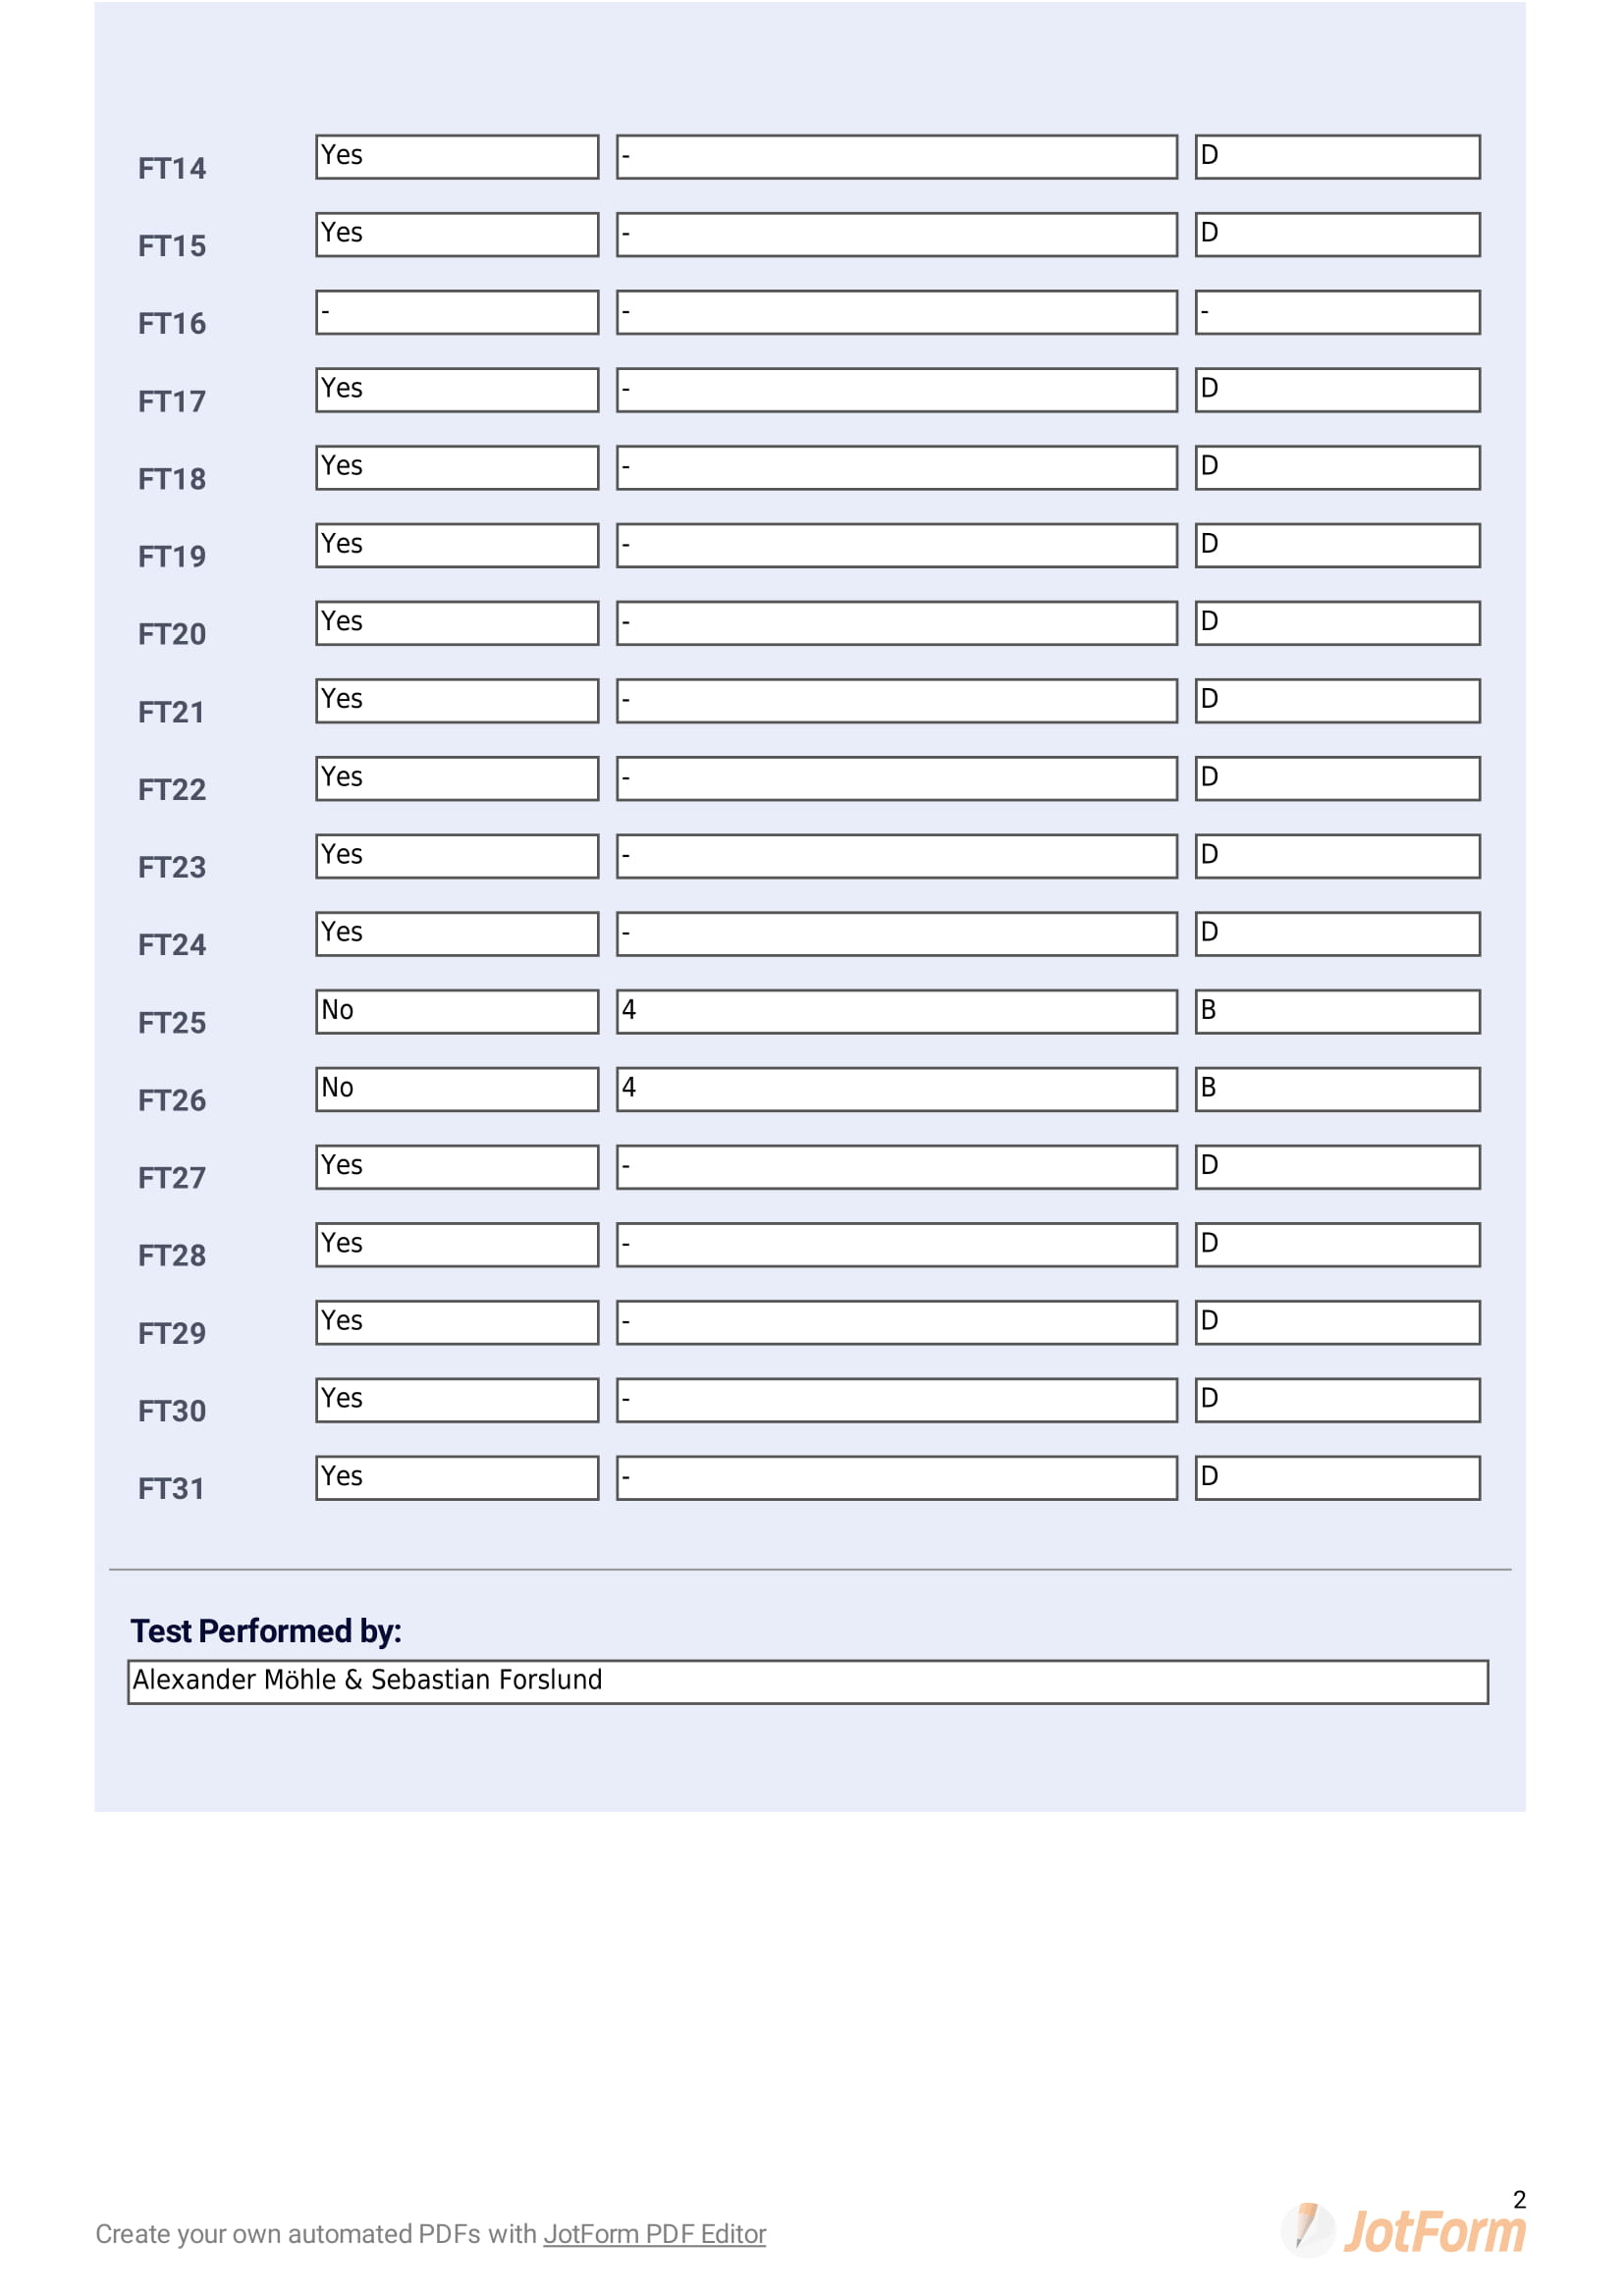
\includegraphics[width=13cm]{images/2021-03-04_Alexander_ST1-2}
     \renewcommand\figurename{Figure}
     \caption{System test form for ST1}
     \label{fig:my_label}
 \end{figure}


\begin{figure}
     \centering
     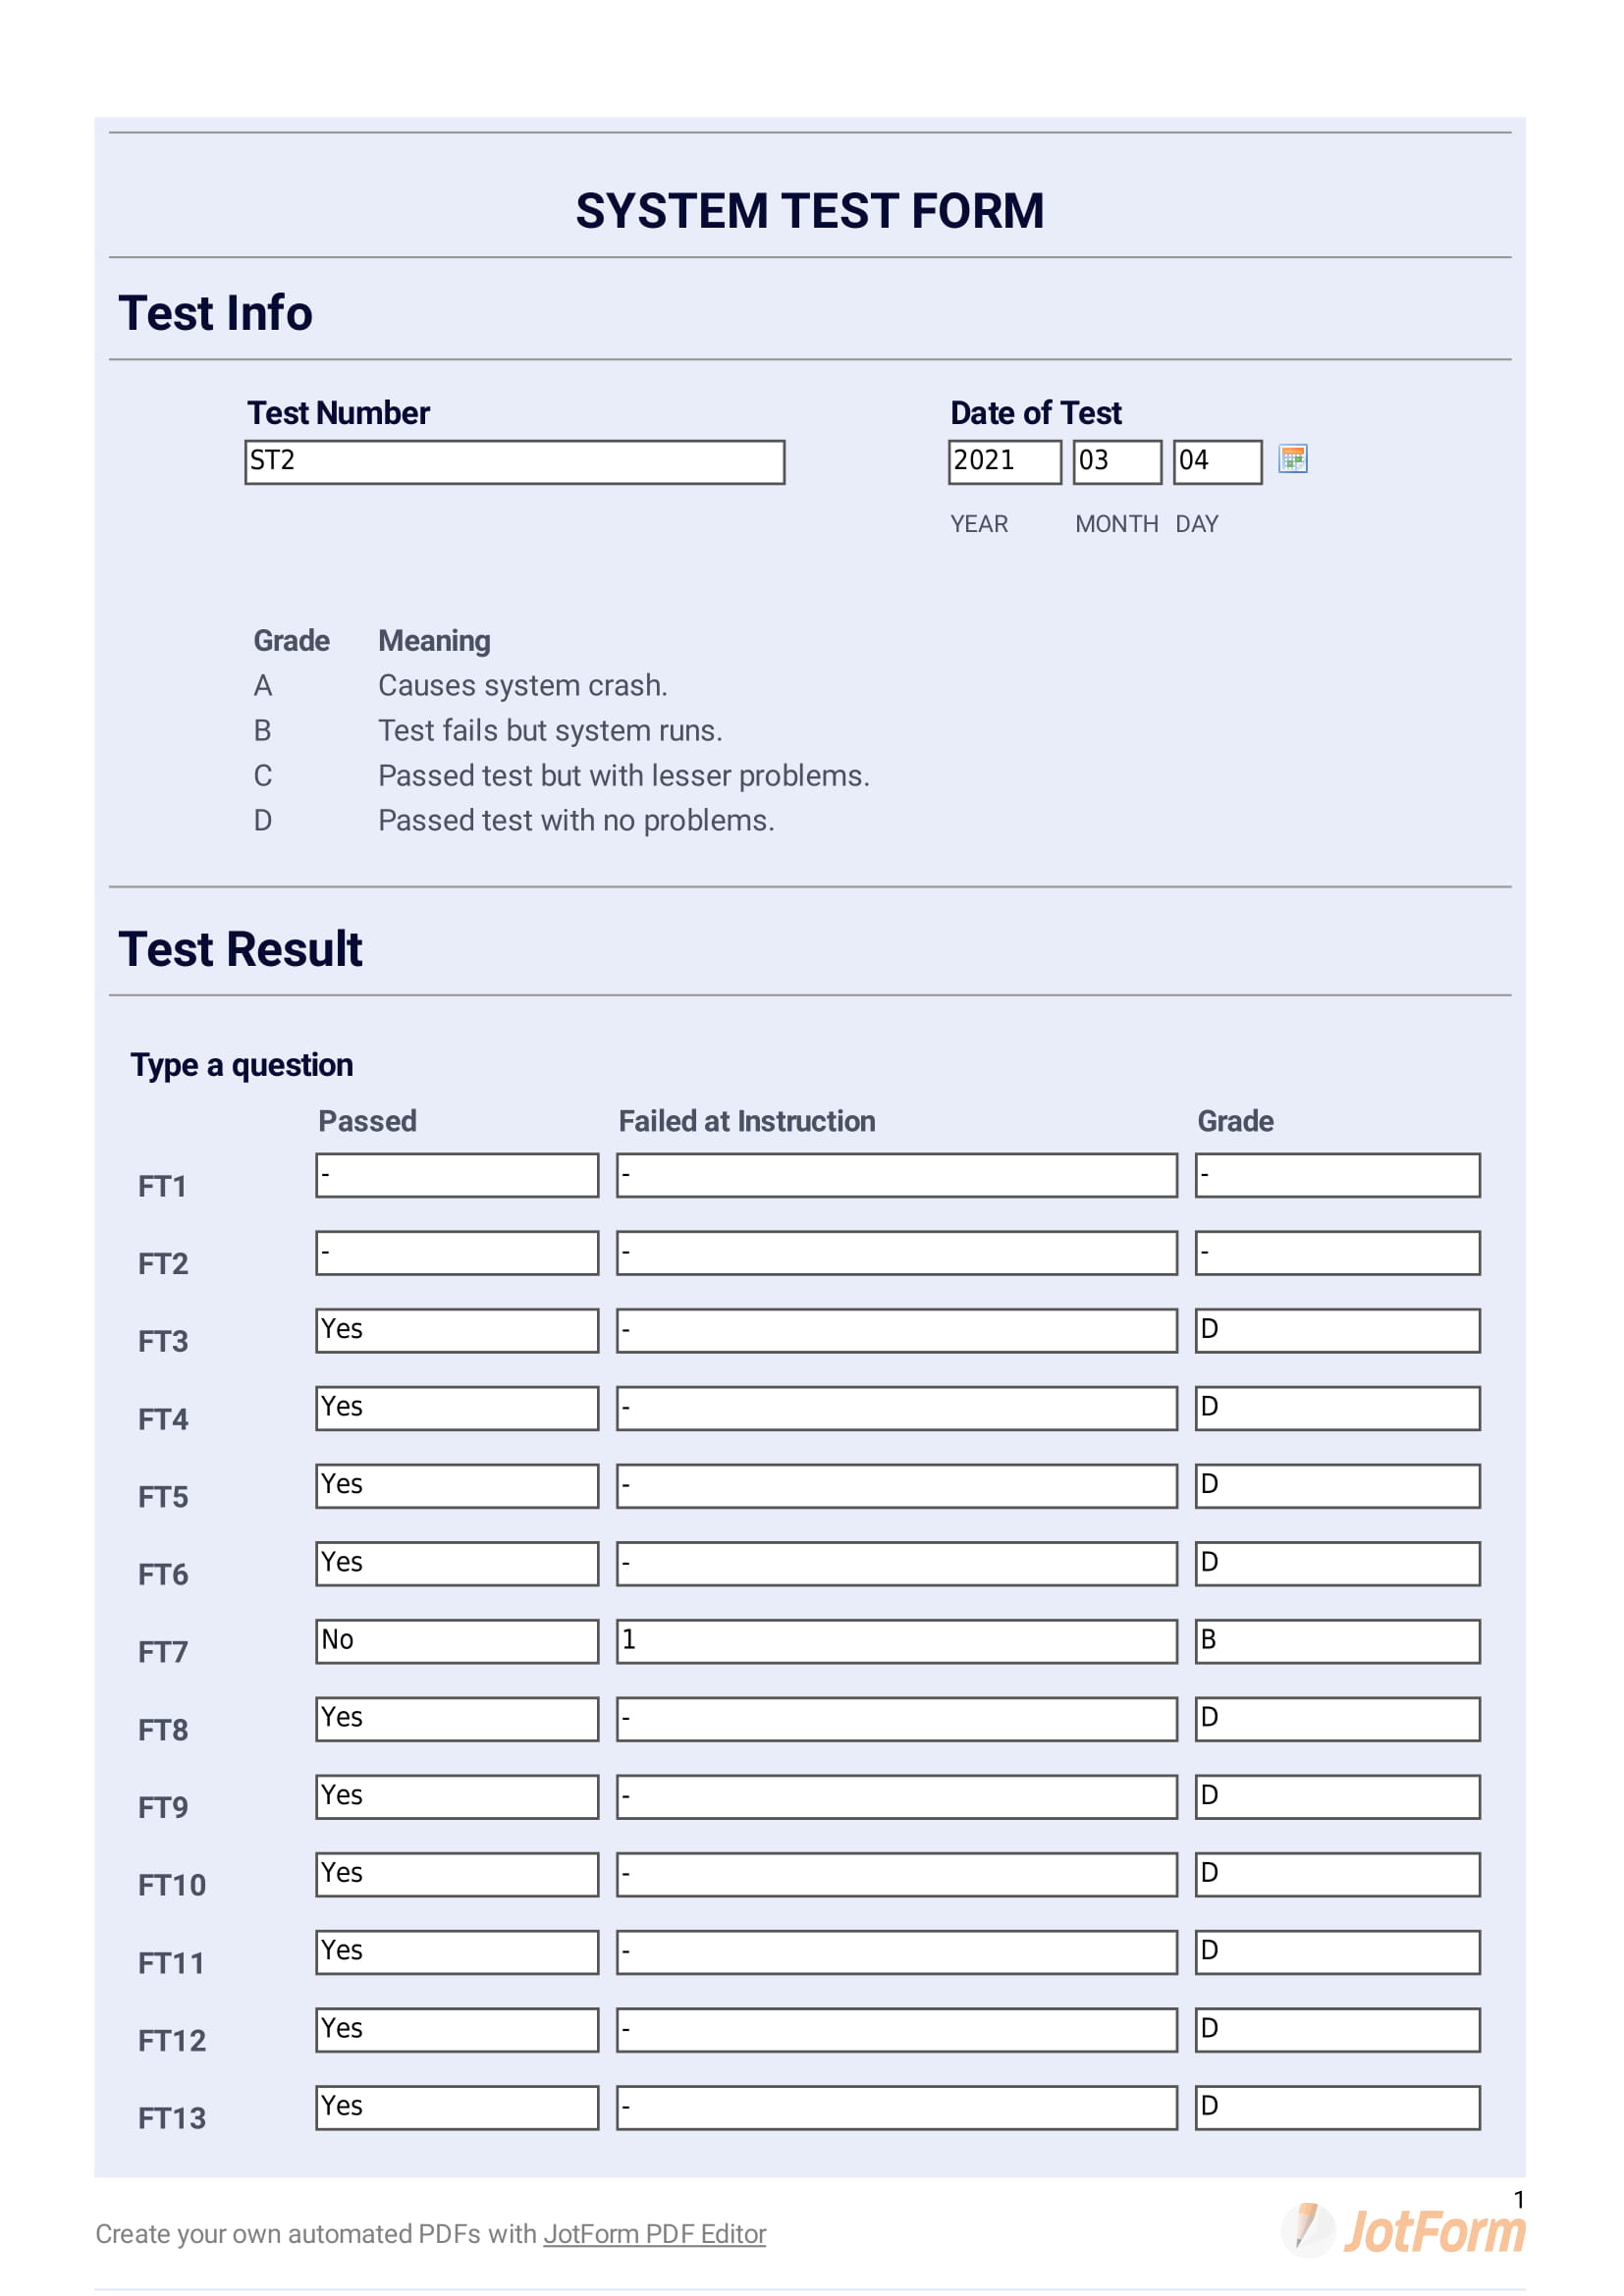
\includegraphics[width=13cm]{images/2021-03-04_Malte_ST2-1}
     \renewcommand\figurename{Figure}
     \label{fig:my_label}
 \end{figure}
 
 \begin{figure}
     \centering
     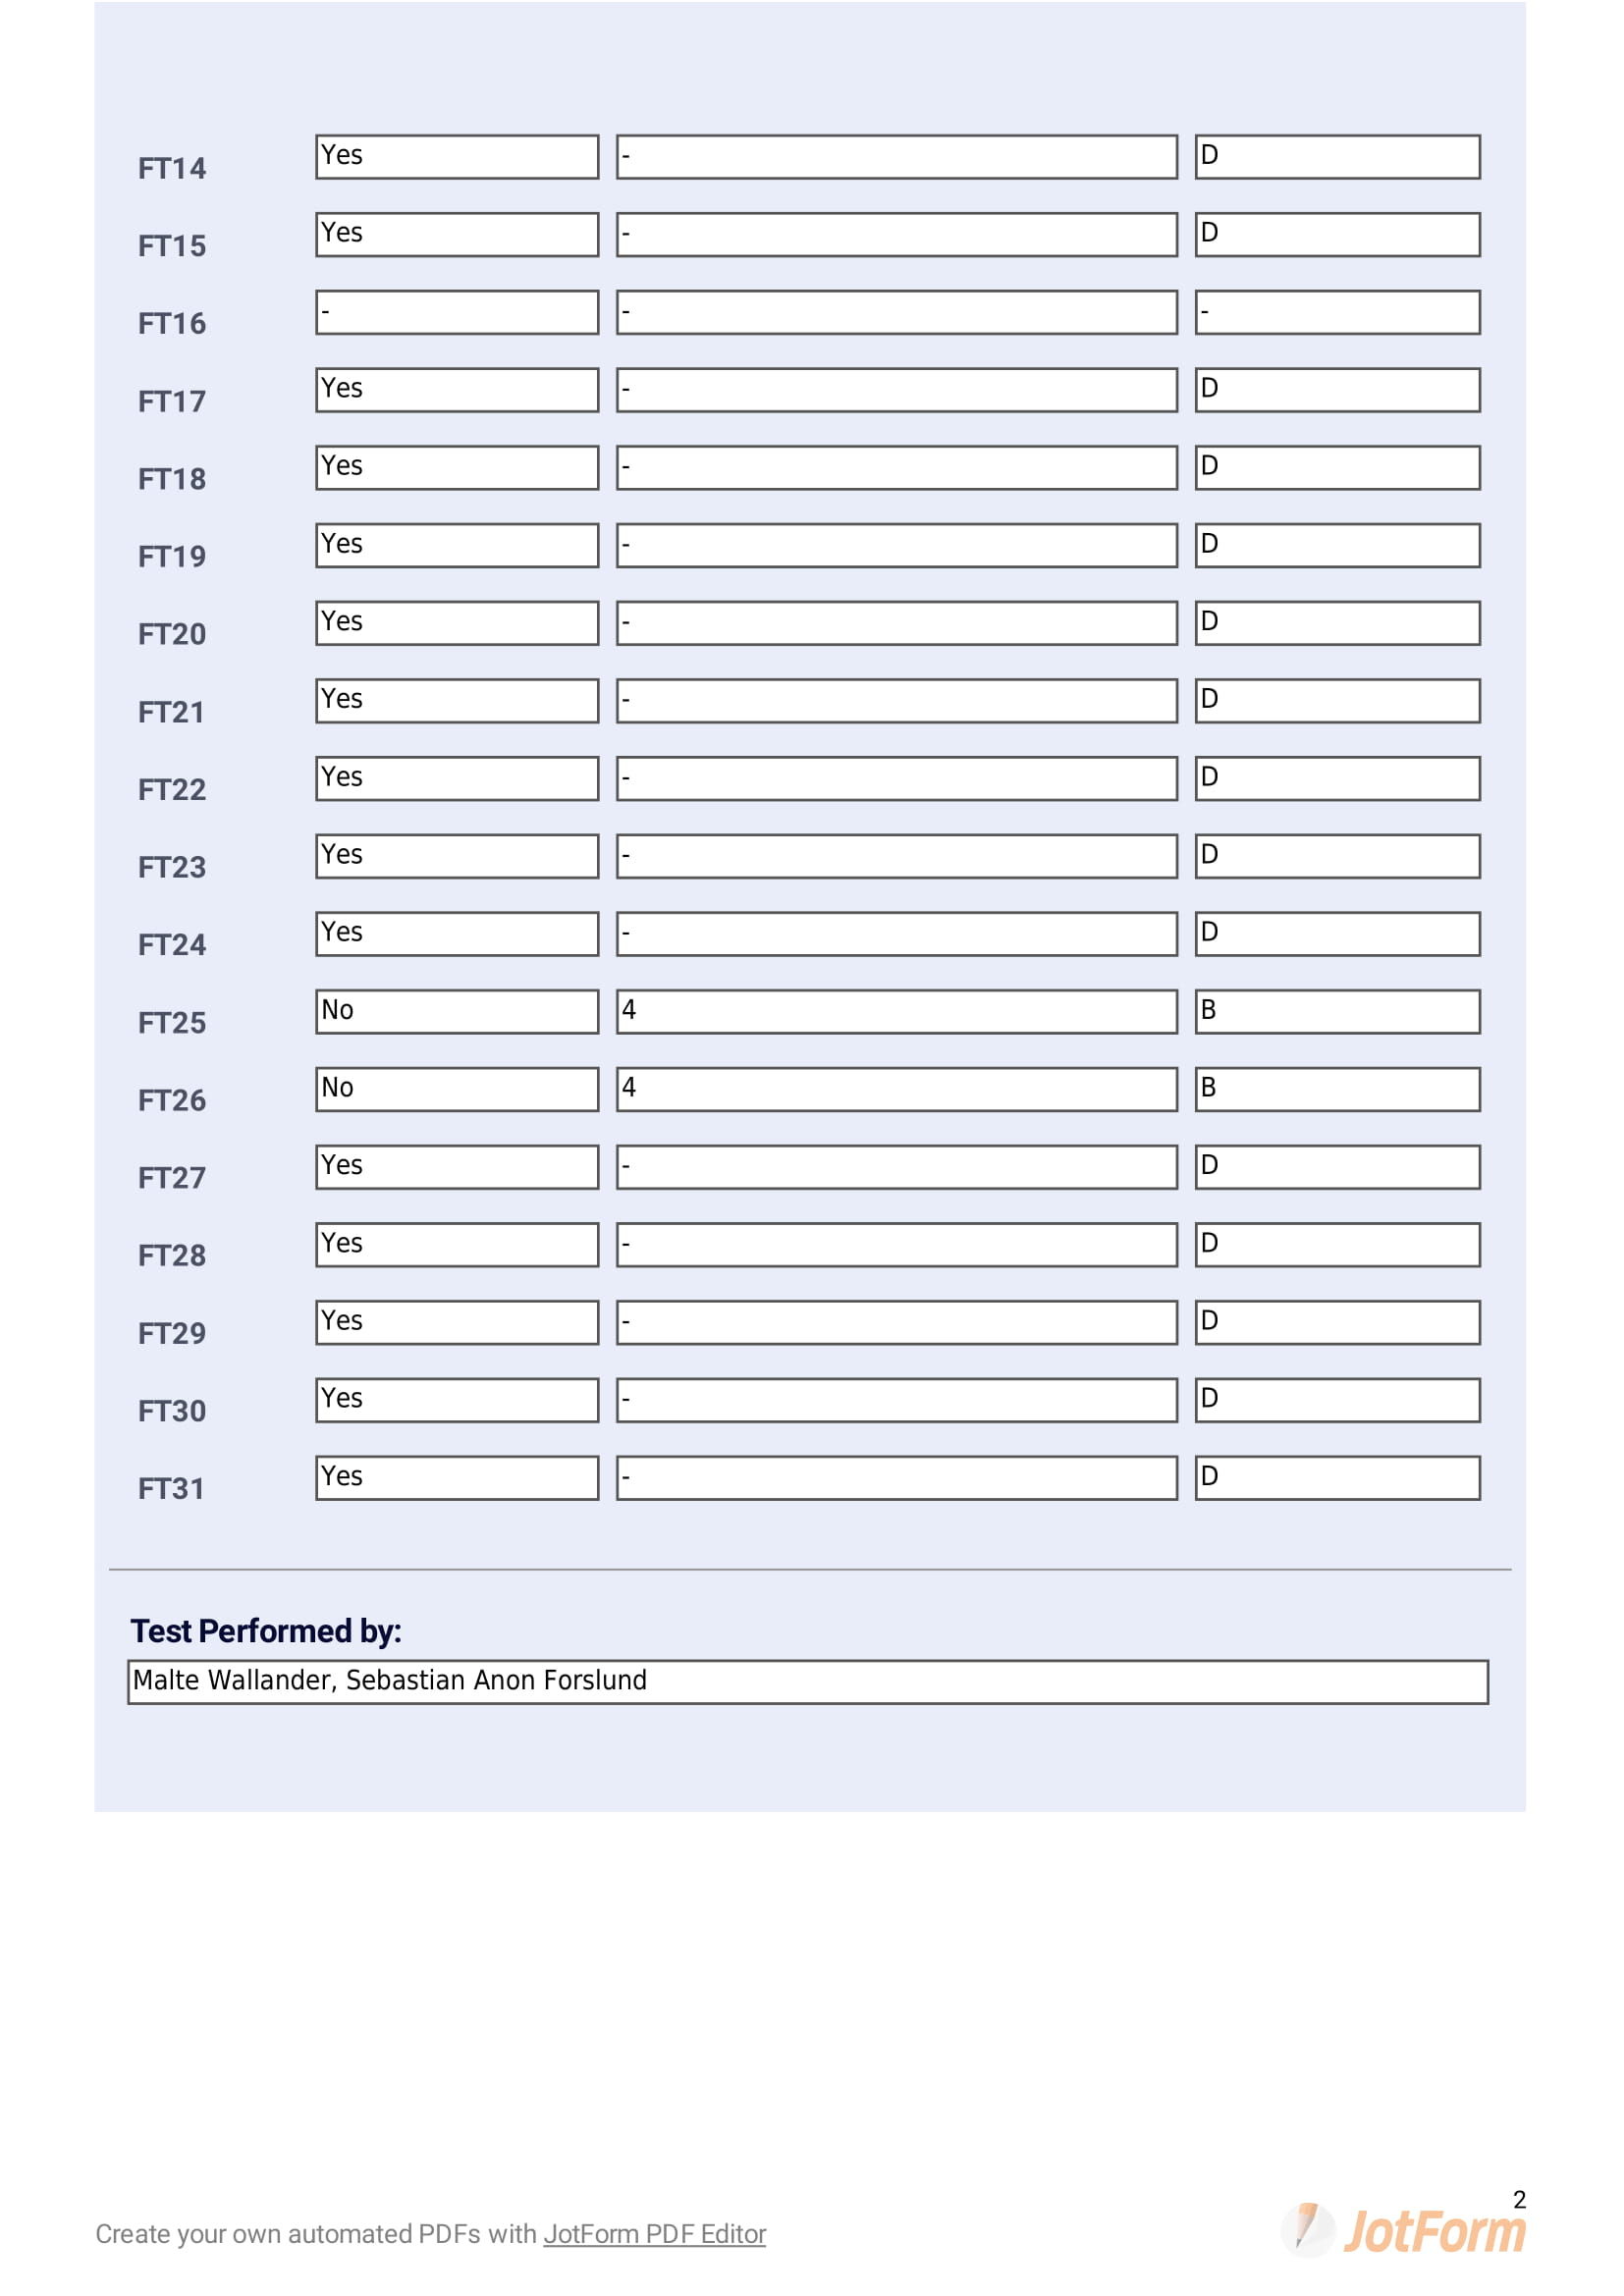
\includegraphics[width=13cm]{images/2021-03-04_Malte_ST2-2}
     \renewcommand\figurename{Figure}
     \caption{System test form for ST2}
     \label{fig:my_label}
 \end{figure}
 

\begin{figure}
     \centering
     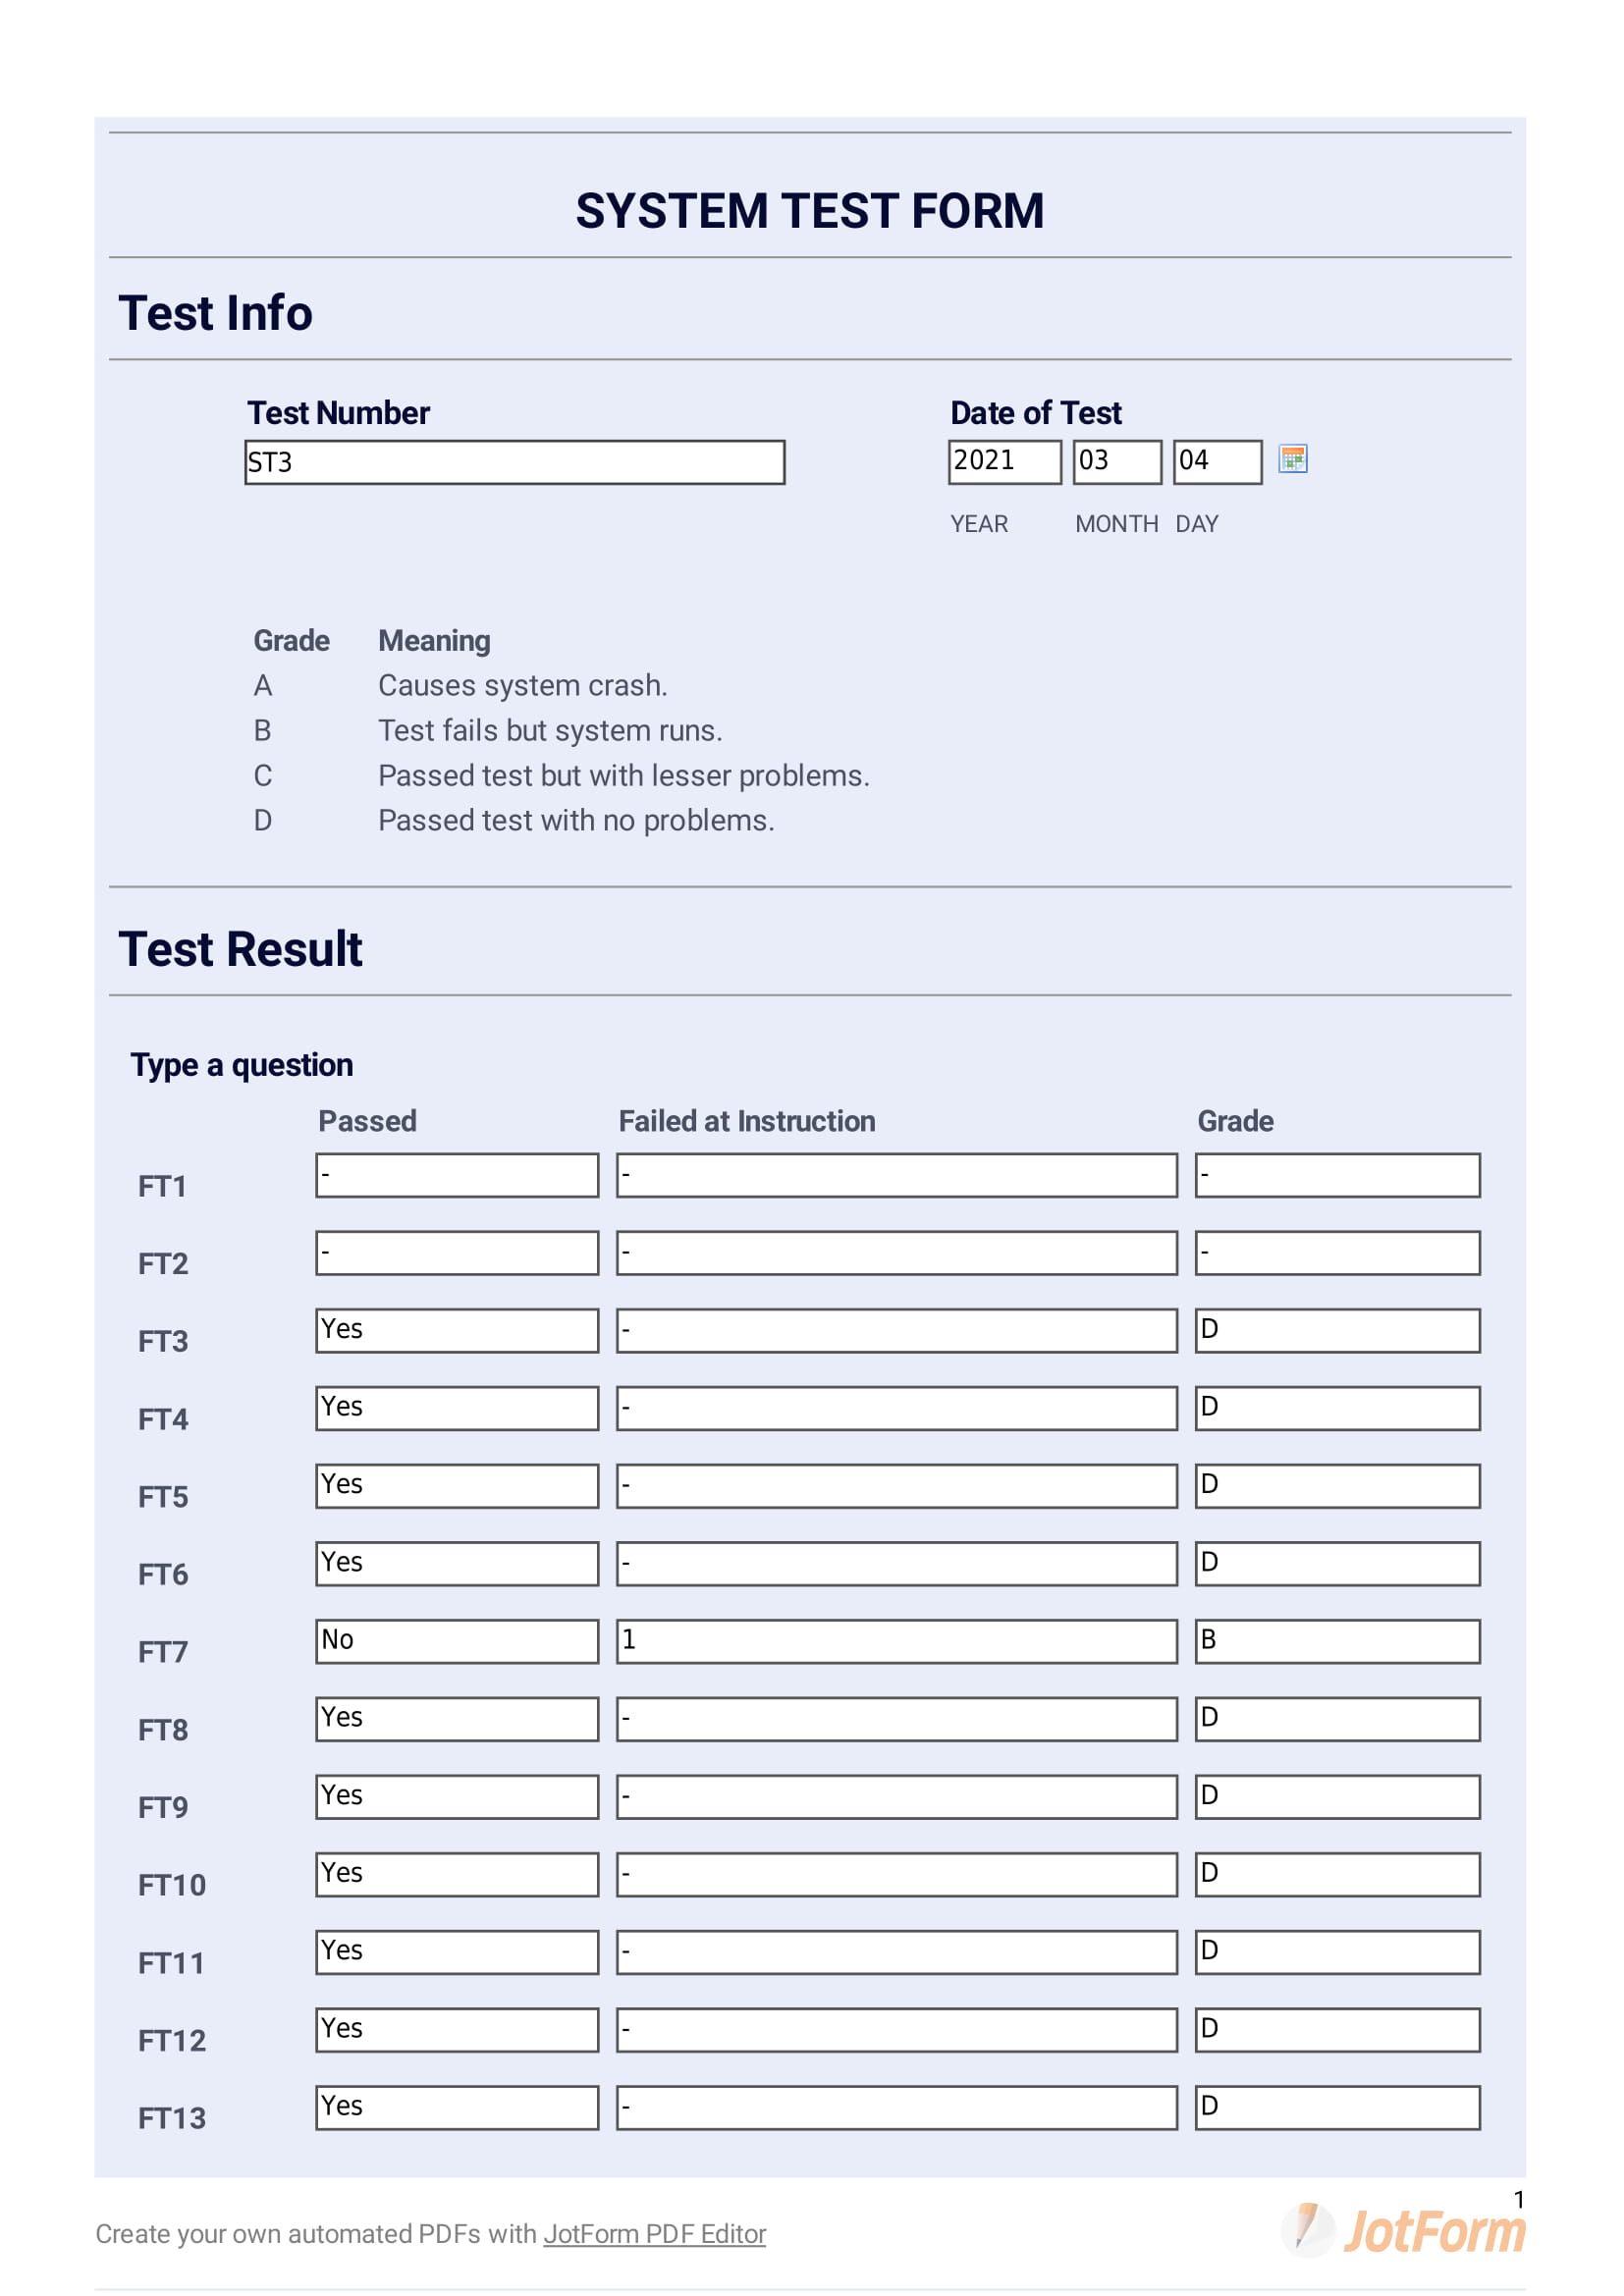
\includegraphics[width=13cm]{images/2021-03-04_Anas_ST3-1}
     \renewcommand\figurename{Figure}
     \label{fig:my_label}
 \end{figure}
 
 \begin{figure}
     \centering
     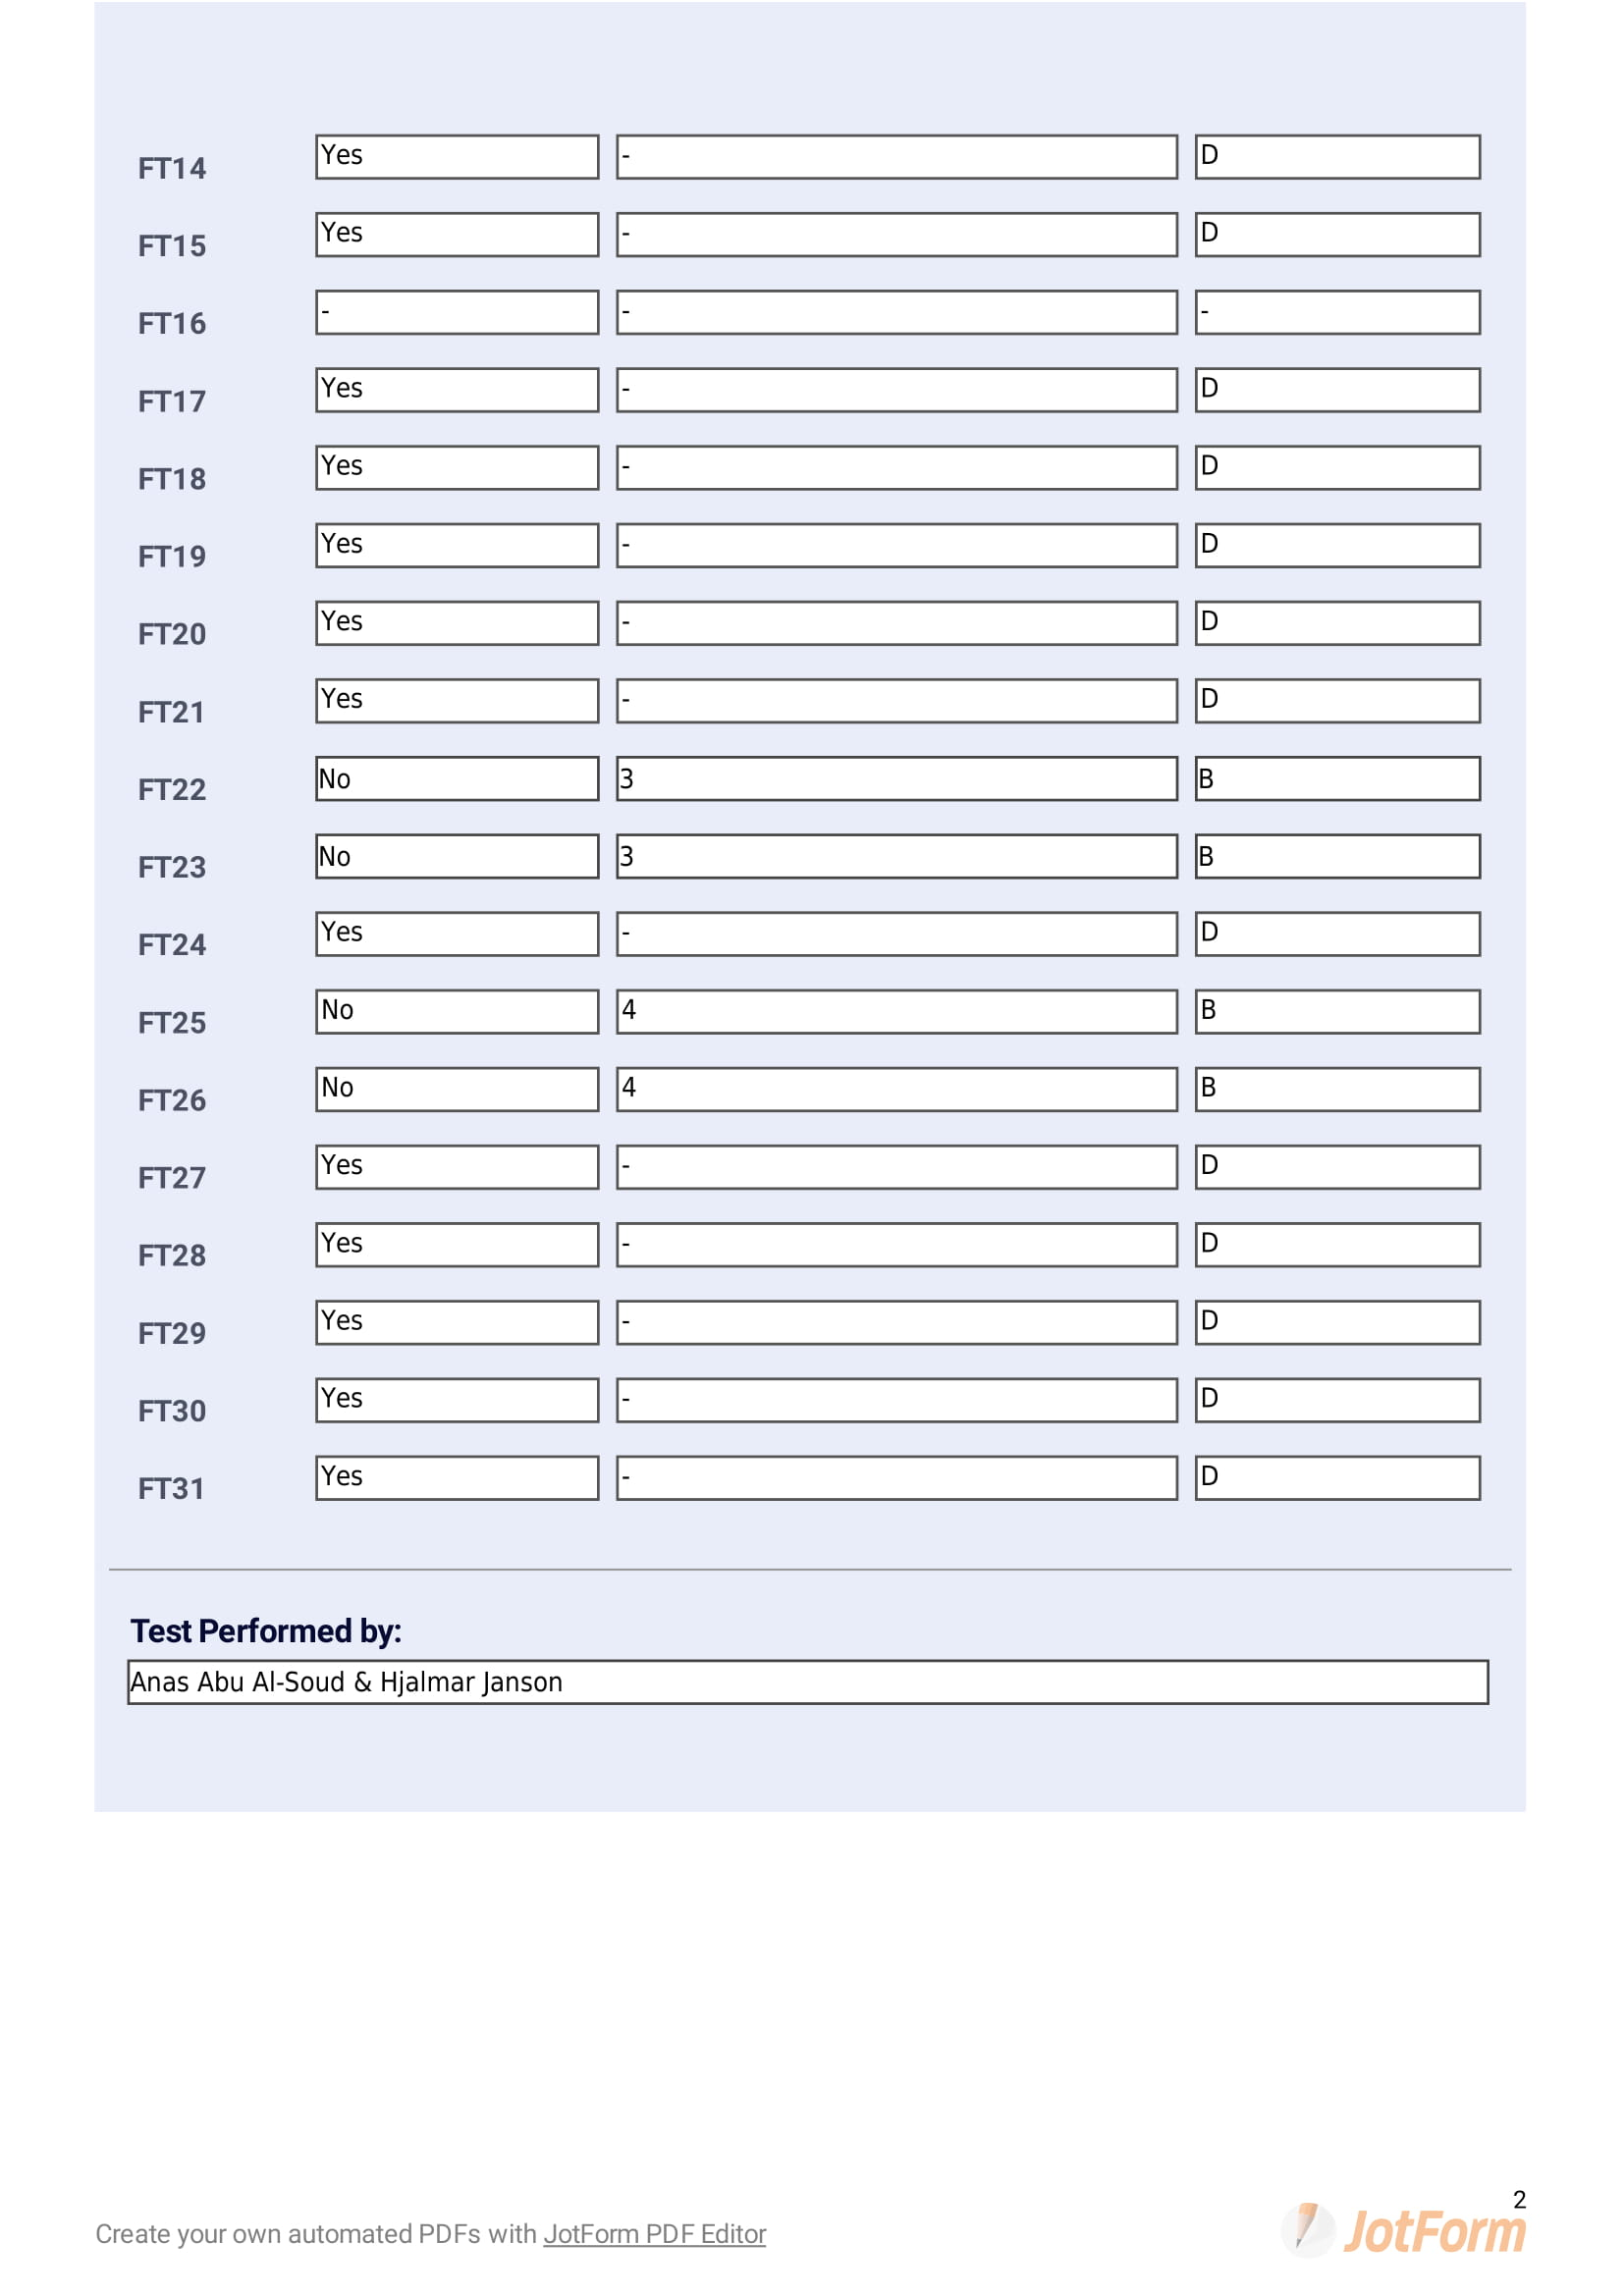
\includegraphics[width=13cm]{images/2021-03-04_Anas_ST3-2}
     \renewcommand\figurename{Figure}
     \caption{System test form for ST2}
     \label{fig:my_label}
 \end{figure}


\newpage
\begin{flushleft}
{\large \textbf{C. Regression Test Result}}
\end{flushleft}

\vspace*{\fill}
                \hfill
                \begin{center}
                This page unintentionally left blank.
                \end{center}
                \vspace{\fill}
                \thispagestyle{empty}

 \begin{figure}
     \centering
     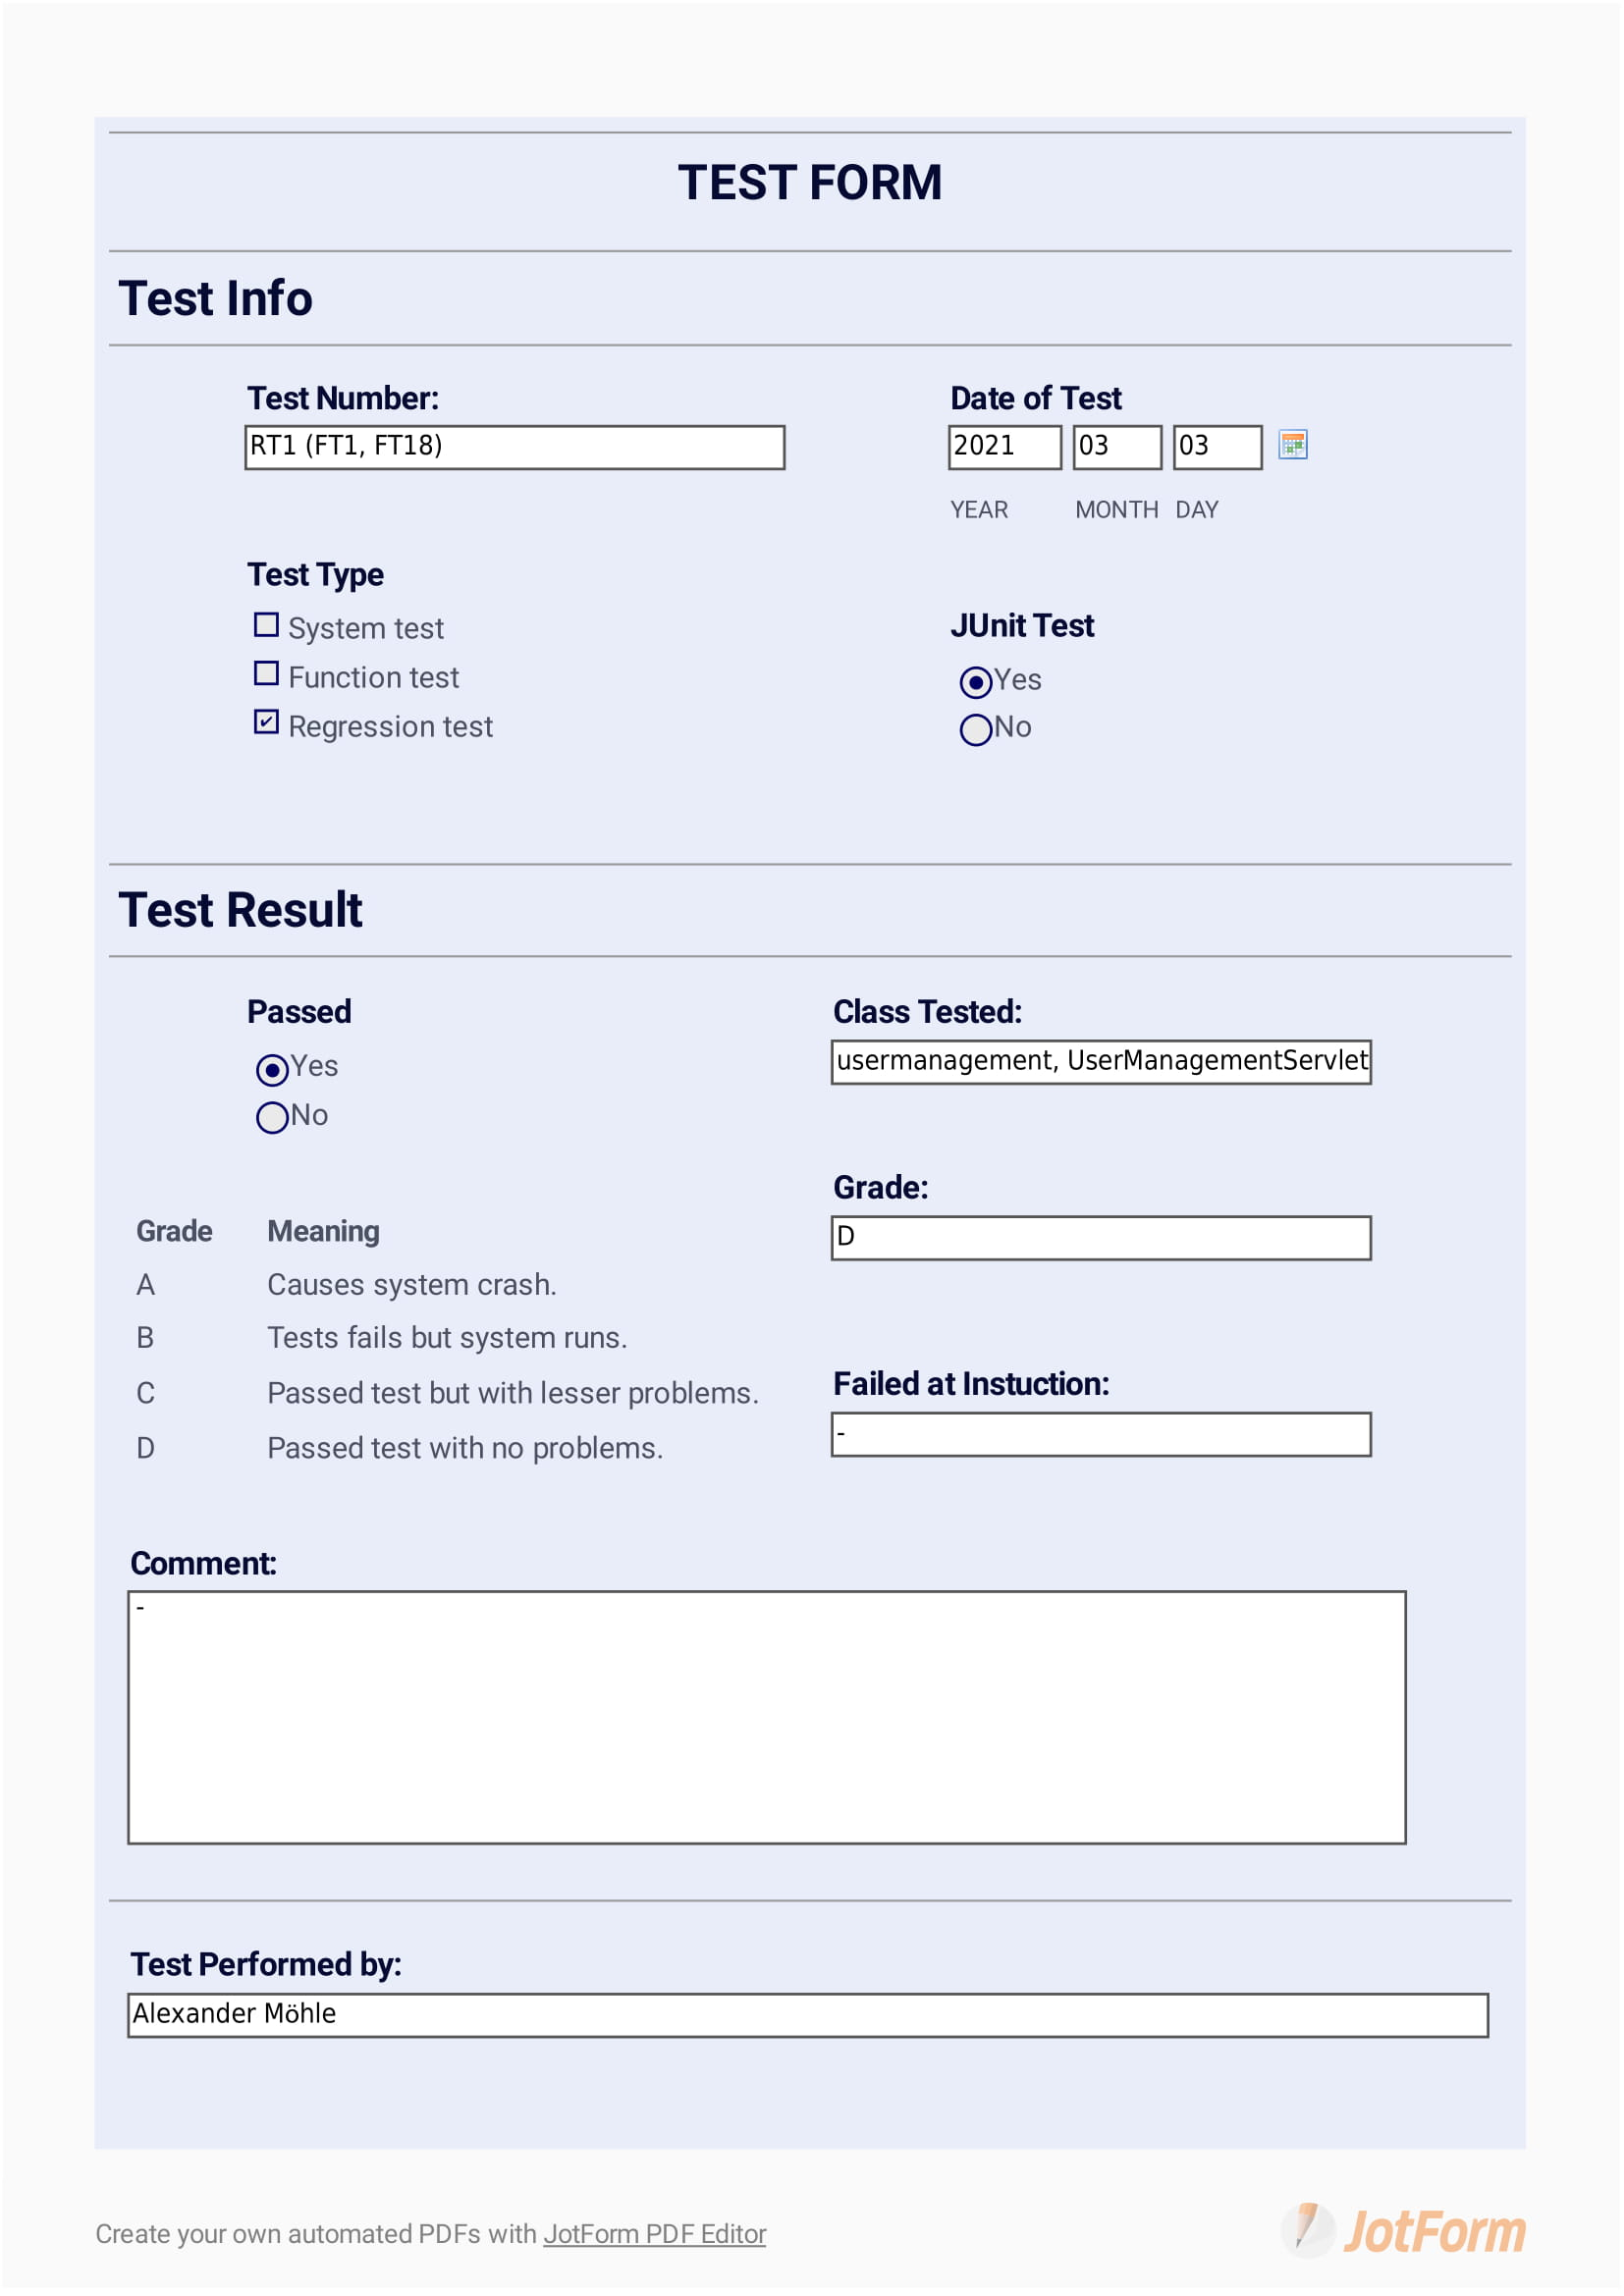
\includegraphics[width=13cm]{images/2021-03-03_Alexander_RT1(FT1, FT18)-1.jpg}
     \renewcommand\figurename{Figure}
     \caption{Regression test form for RT1 (FT1,FT18)}
     \label{fig:my_label}
 \end{figure}
 
  \begin{figure}
     \centering
     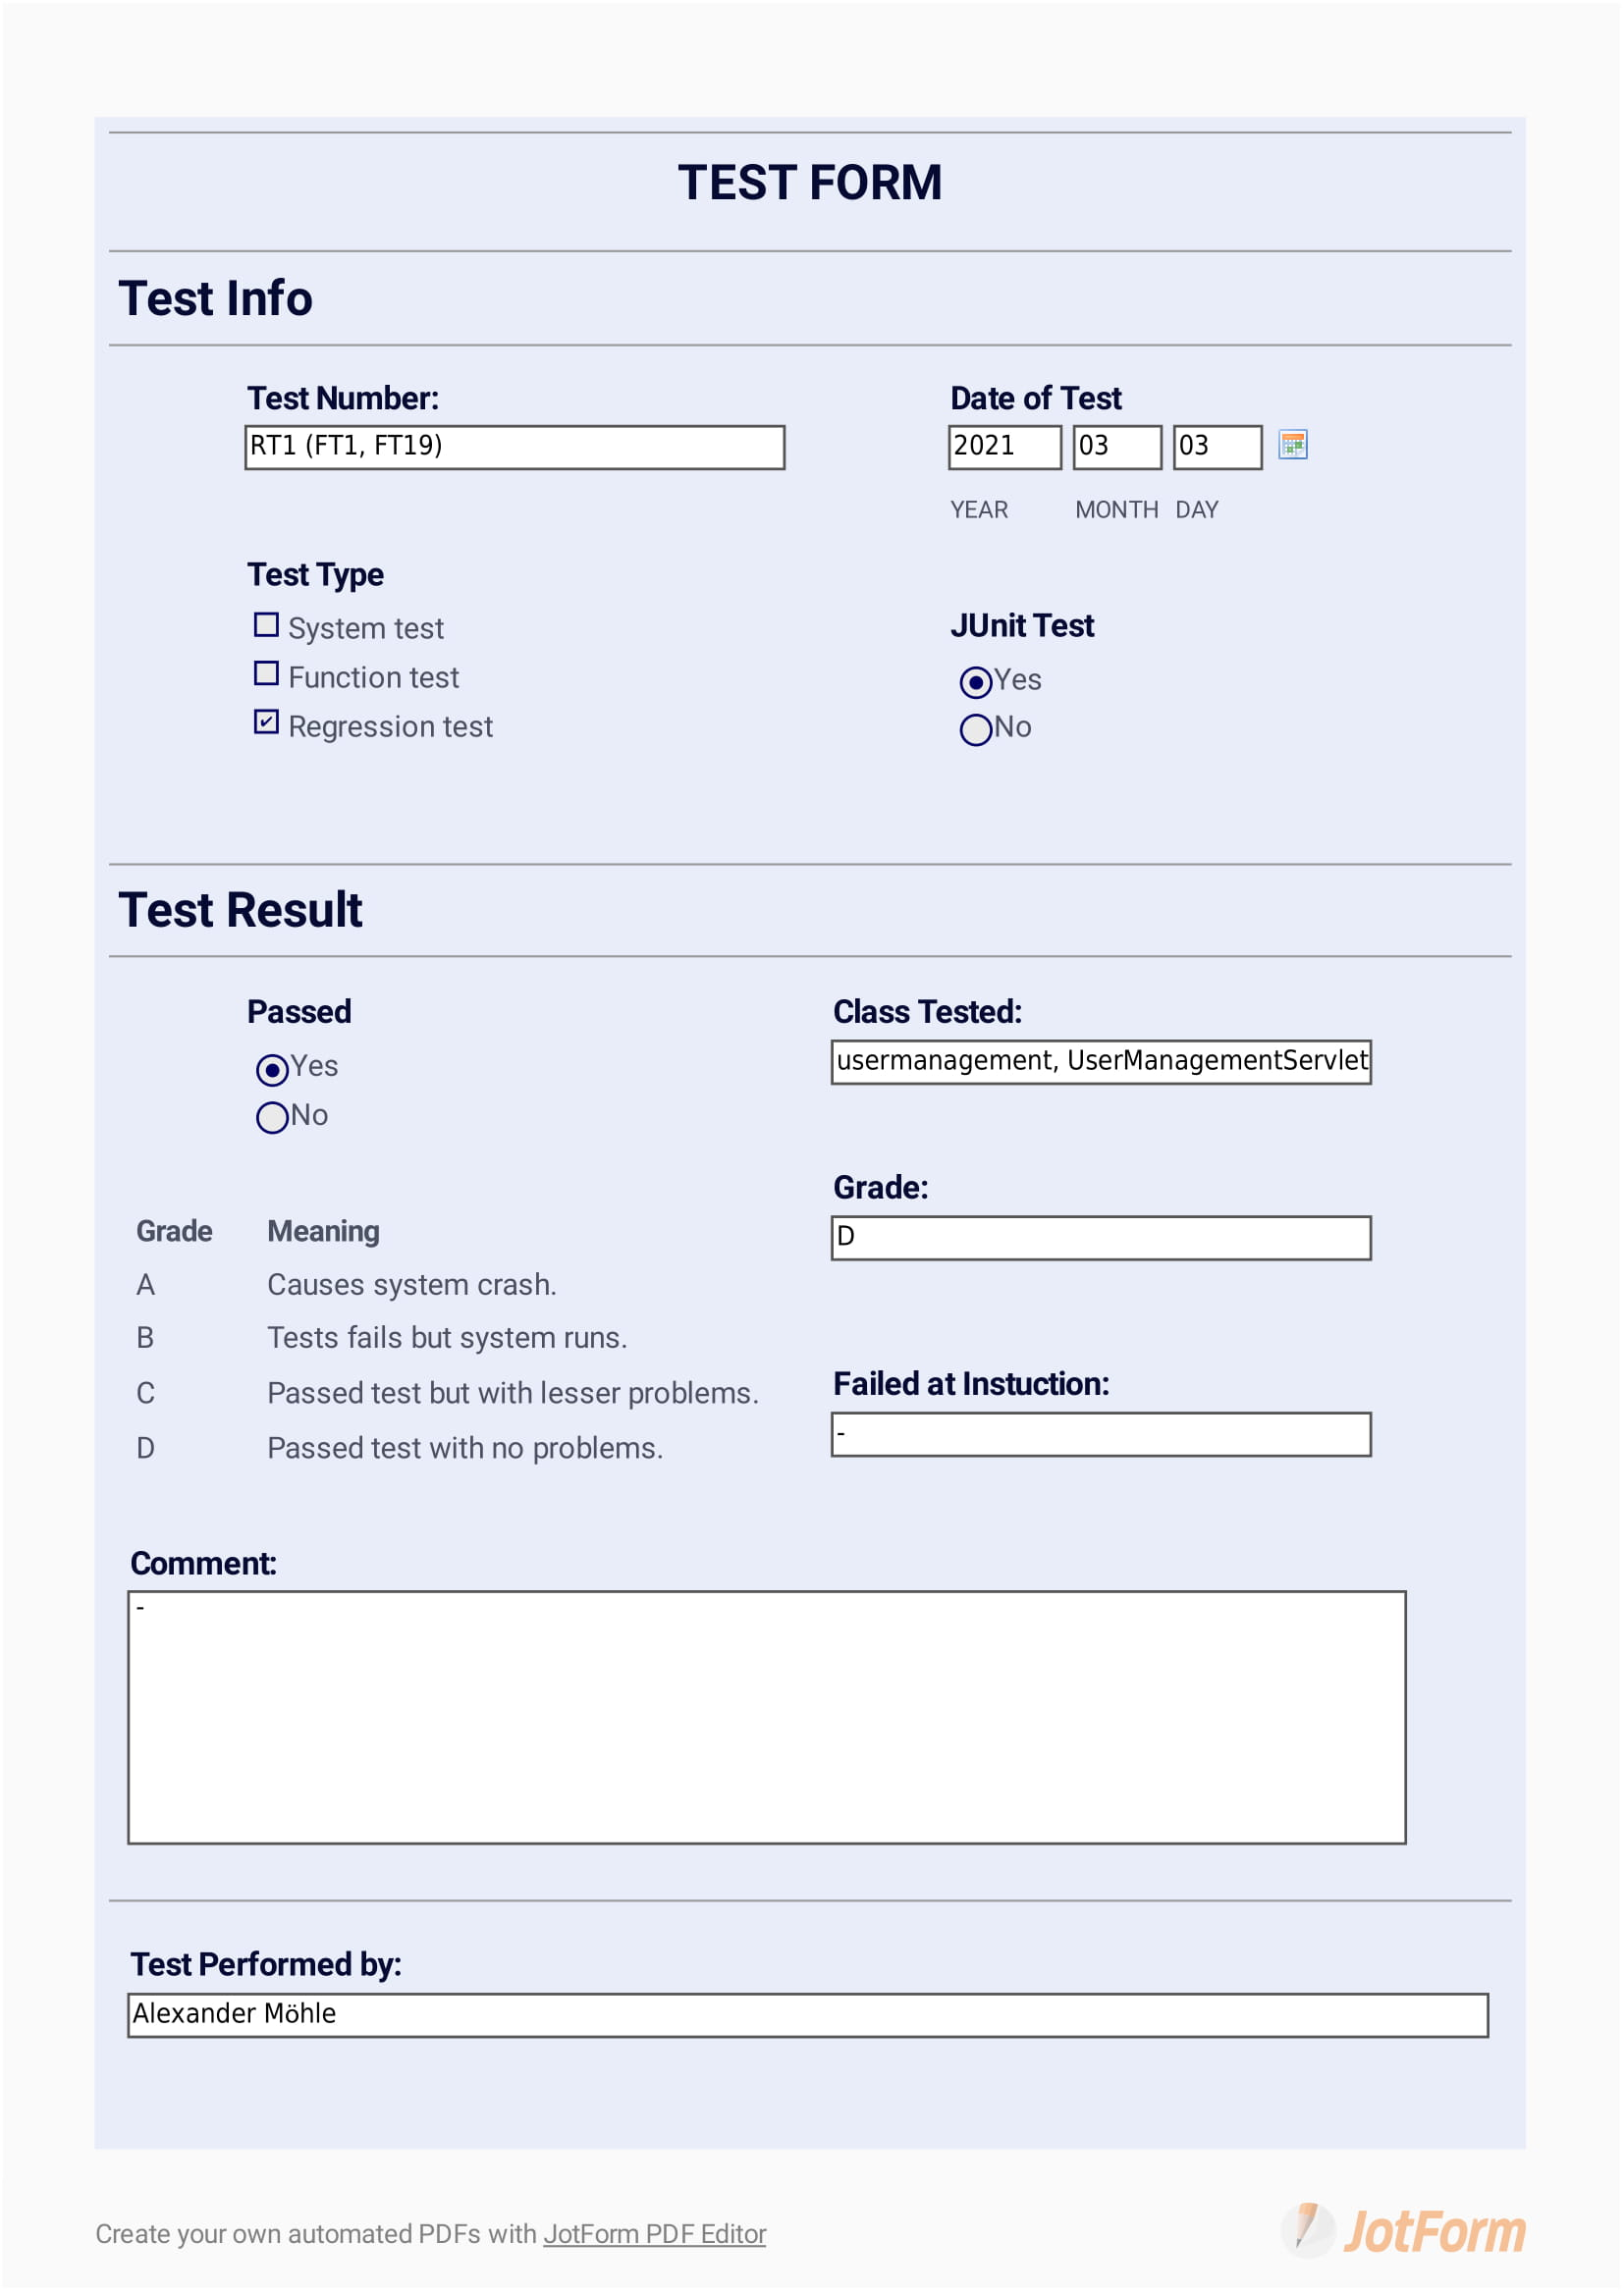
\includegraphics[width=13cm]{images/2021-03-03_Alexander_RT1(FT1, FT19)-1.jpg}
     \renewcommand\figurename{Figure}
     \caption{Regression test form for RT1 (FT1,FT19)}
     \label{fig:my_label}
 \end{figure}
 
  \begin{figure}
     \centering
     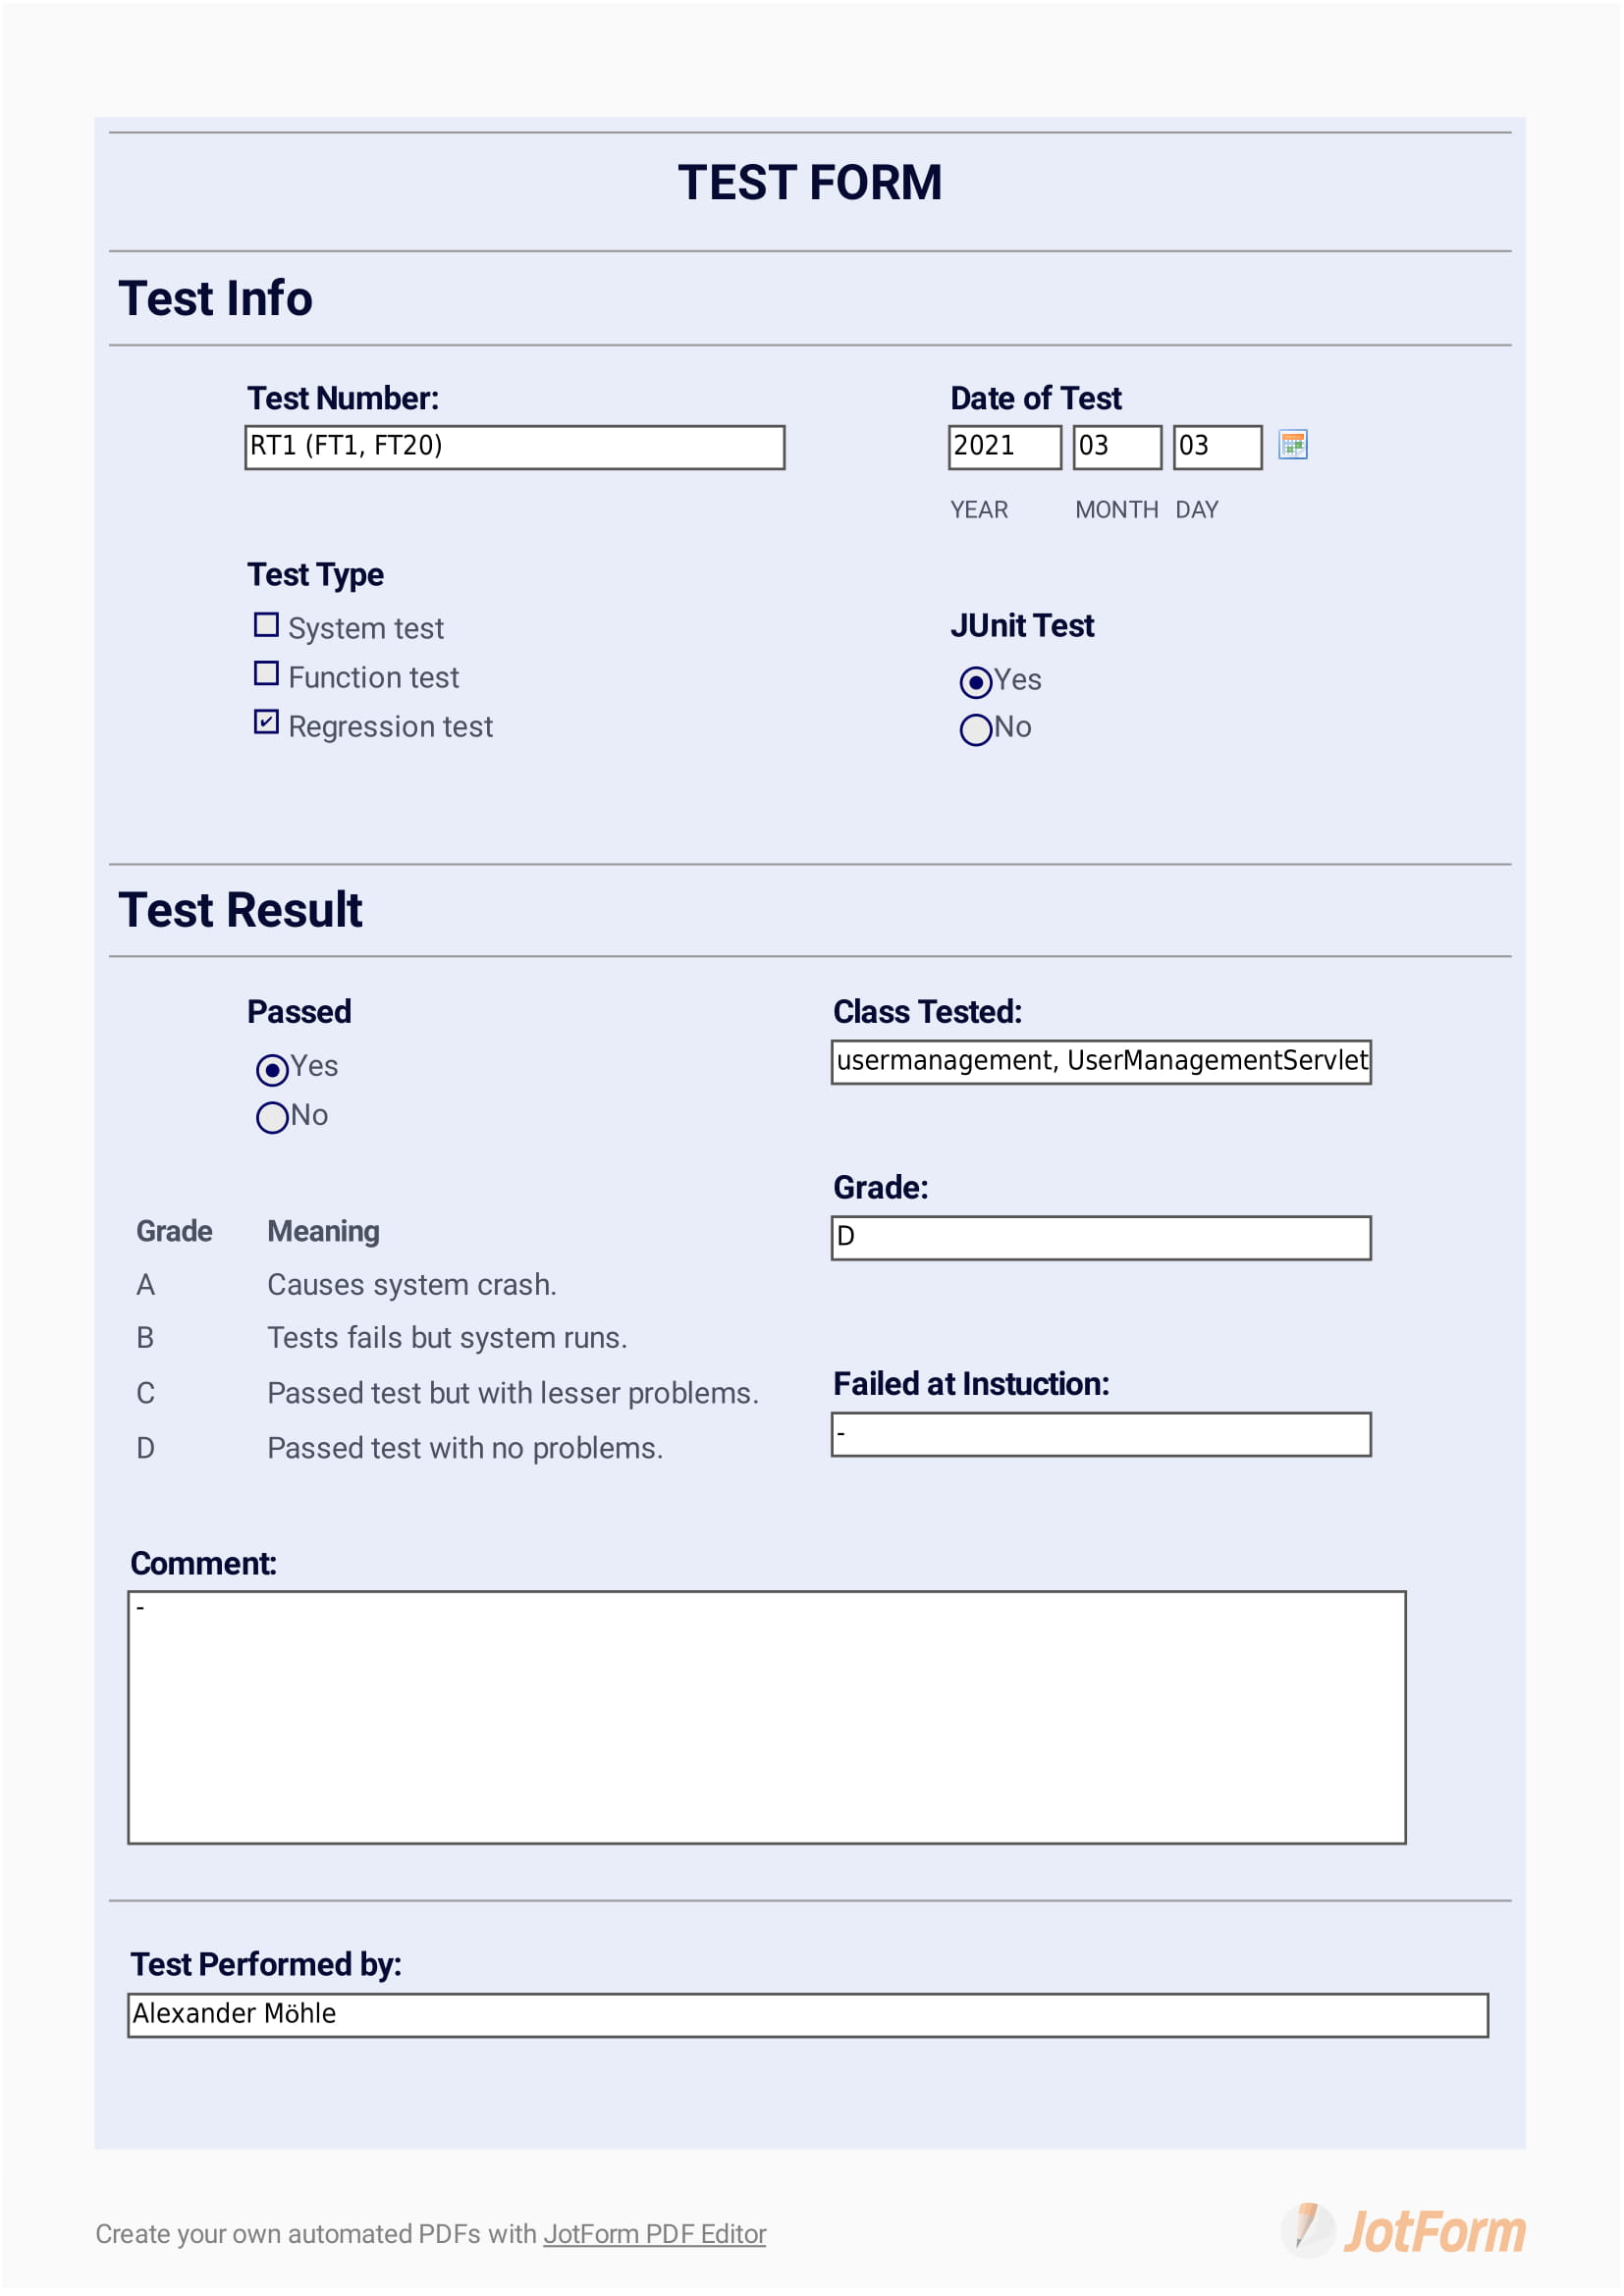
\includegraphics[width=13cm]{images/2021-03-03_Alexander_RT1(FT1, FT20)-1.jpg}
     \renewcommand\figurename{Figure}
     \caption{Regression test form for RT1 (FT1,FT20)}
     \label{fig:my_label}
 \end{figure}
 
  \begin{figure}
     \centering
     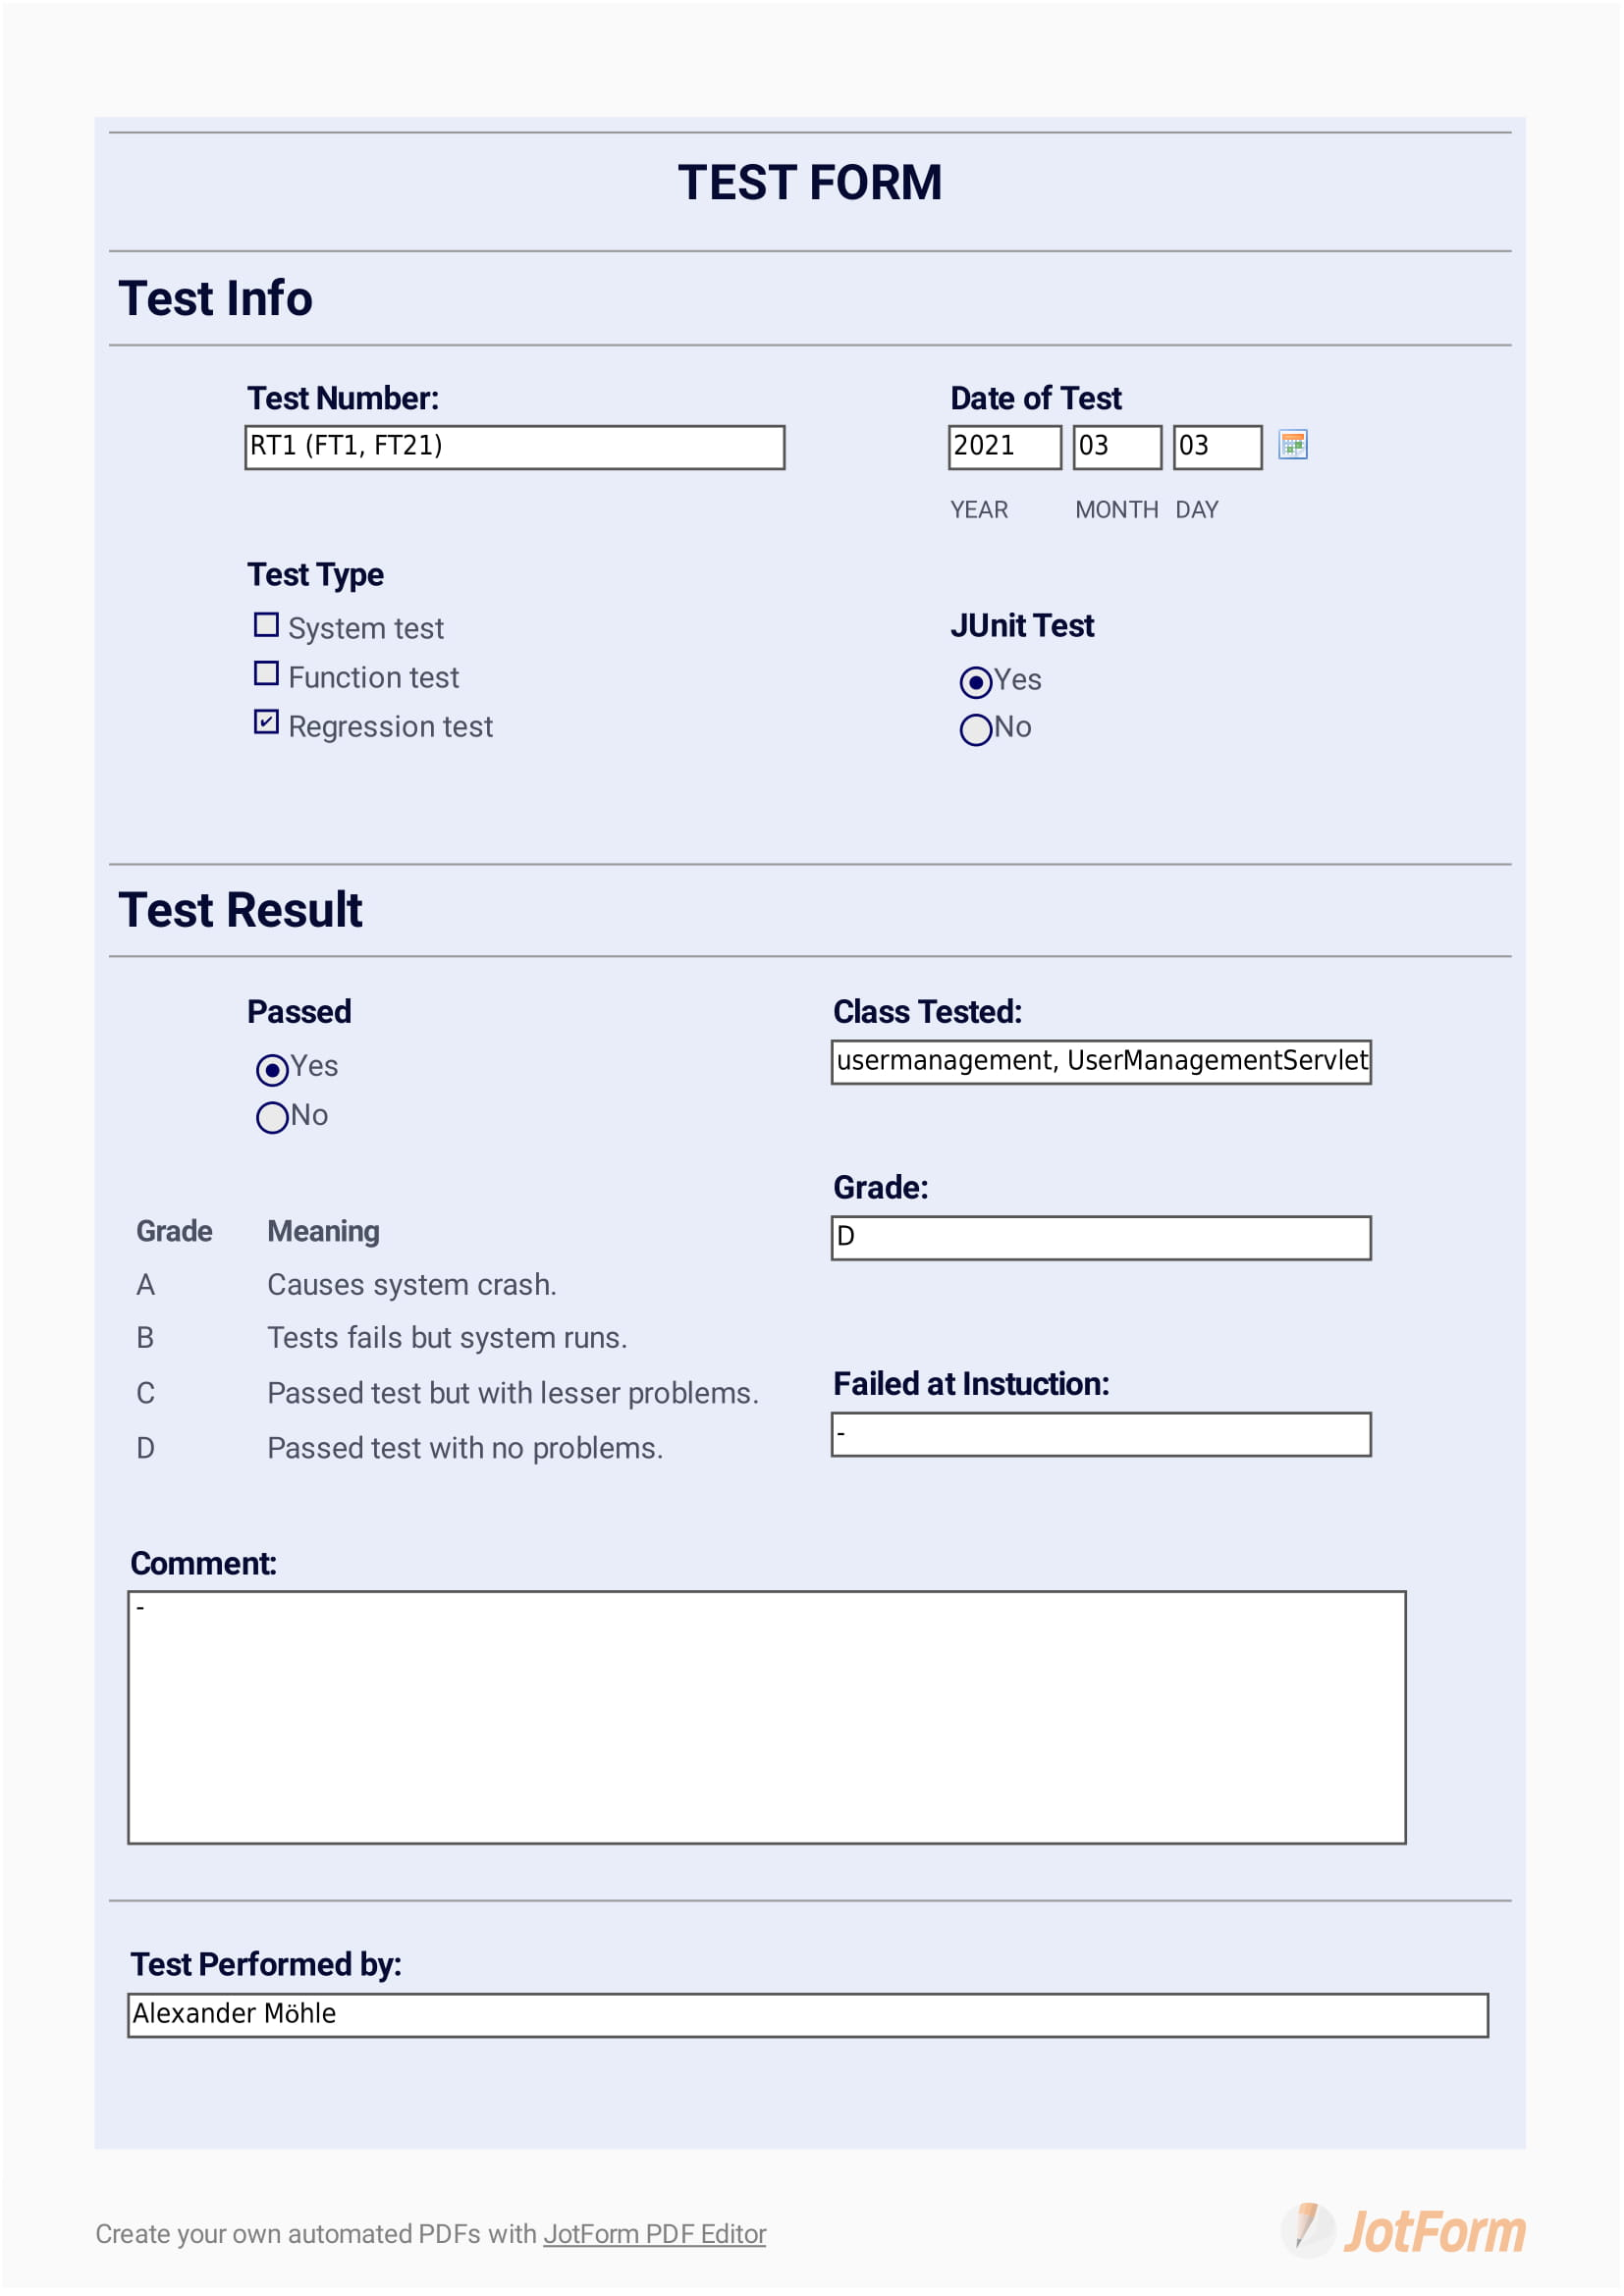
\includegraphics[width=13cm]{images/2021-03-03_Alexander_RT1(FT1, FT21)-1.jpg}
     \renewcommand\figurename{Figure}
     \caption{Regression test form for RT1 (FT1,FT21)}
     \label{fig:my_label}
 \end{figure}


\newpage
\begin{flushleft}
{\large \textbf{D. Test Result in Google Sheet}}
\end{flushleft}

\newpage
\begin{flushleft}
{\large \textbf{E. Review Protocols}}
\end{flushleft}


%---------Document ends here-----------

\end{document}
